  \documentclass[10pt,aspectratio=169]{beamer}

\usetheme[progressbar=frametitle]{metropolis}

\makeatletter
% \setlength{\metropolis@titleseparator@linewidth}{1pt}
\setlength{\metropolis@progressonsectionpage@linewidth}{0.7pt}
\setlength{\metropolis@progressinheadfoot@linewidth}{0.7pt}
\makeatother

\usepackage{appendixnumberbeamer}
\usepackage[absolute,overlay]{textpos}
\usepackage{booktabs}
\usepackage[scale=2]{ccicons}
\usepackage{tikz}
\usepackage{pgfplots}
\usepackage{listings}
\usepgfplotslibrary{dateplot}

\usepackage{xspace}
\newcommand{\themename}{\textbf{\textsc{metropolis}}\xspace}
\usecolortheme{default}
% Colores defined
\usepackage{color, colortbl}
\definecolor{White}{HTML}{ffffff}
\definecolor{Blue}{HTML}{183354}
\definecolor{Gray}{HTML}{e6e6e6} % d6d6d6
\definecolor{Orange}{HTML}{ff8000}
\definecolor{OrangeBackground}{HTML}{fff3e6}
\definecolor{BlueBorder}{HTML}{345eeb}
\definecolor{BlueBackground}{HTML}{dee8fc}

\definecolor{dkgreen}{rgb}{0,0.6,0}
\definecolor{gray}{rgb}{0.5,0.5,0.5}
\definecolor{mauve}{rgb}{0.58,0,0.82}
\definecolor{Purple}{HTML}{6f42c1}
\definecolor{darkgray}{RGB}{96, 98, 99}
\definecolor{darkred}{RGB}{145, 29, 16}


% Some boxes
\setbeamercolor{coloredboxstuff}{fg=black,bg=Gray}
\setbeamercolor{boxorange}{fg=black,bg=Orange}

% Change colores template
\setbeamercolor{background canvas}{bg=White}
\setbeamercolor{title}{fg=Blue}
\setbeamercolor{frametitle}{bg=Blue}
\setbeamercolor{item}{fg=orange}
\setbeamercolor{normal text}{fg=black}
\usebeamercolor[fg]{normal text}

\newcommand<>{\reveal}[1]{\mbox{}\visible#2{#1}}

\newcommand\Fontvi{\fontsize{10}{7.2}\selectfont}
\newcommand\Fonteight{\fontsize{9pt}{7.2}\selectfont}


\usepackage{lmodern,amsmath,amssymb}
\usepackage[beamer]{hf-tikz}
\usepackage{xcolor}
\usepackage{soul}
\newcommand{\hll}[1]{\colorbox{orange!10}{$\displaystyle #1$}}

\addtobeamertemplate{title}{\vskip-10.5ex}{}

\usepackage{listings}
\lstset{
	language=R,
	aboveskip=3mm,
	belowskip=3mm,
	showstringspaces=false,
	belowskip=0.15cm,
	% belowcaptionskip=0\baselineskip,
	columns=fullflexible,
	basicstyle={\fontsize{8}{9.6}\ttfamily},
	frame=single,
	xleftmargin=3mm,
	xrightmargin=1mm,
	% framerule=1pt,
	rulecolor=\color{black},
	numbers=left,
	stepnumber=1,
	numbersep=5pt,
	tabsize=2,
	numberstyle=\tiny\color{darkred},
	keywordstyle=\color{Purple},
	commentstyle=\color{darkgray},
	stringstyle=\color{dkgreen},
	breaklines=true,
	breakatwhitespace=false,
	captionpos=b,
	deletekeywords={
		model, 
		data, 
		example,
		single, 
		real, 
		min, 
		frame, 
		file, 
		by, 
		log, 
		density, 
		labels,
		cov,
		\_,
		se
	},
	morekeywords={
		deconvDigitalDLSorter, 
		deconvDigitalDLSorterObj, 
		loadRealSCProfiles, 
		loadFinalSCProfiles, 
		estimateZinbwaveParams, 
		simSingleCellProfiles, 
		generateTrainAndTestBulkProbMatrix, 
		install\_, 
		github,
		showProbPlot,
		generateBulkSamples,
		loadDeconvData,
		prepareDataForTraining,
		trainDigitalDLSorterModel,
		calculateEvalMetrics,
		barPlotCellTypes,
		distErrorPlot,
		corrExpPredPlot,
		blandAltmanLehPlot,
		barErrorPlot,
		loadDeconvDataFromSummarizedExperiment
	}
}

\usepackage{tikz}
\usetikzlibrary{shapes,arrows,positioning}

\newsavebox\blockbox
\newenvironment{highlightblock}{%
  \begin{lrbox}{\blockbox}%
    \begin{minipage}{.9\textwidth}
}{
    \end{minipage}
  \end{lrbox}
  \tikz\node[
    fill=OrangeBackground,
    draw=Orange,
    line width=1pt,
    inner sep=7.5pt,
    % rounded corners,
    outer sep=0pt,
    text centered
  ]{\usebox\blockbox};
}


\usepackage{hyperref}
\hypersetup{
    colorlinks=true,
    linkcolor=black,
    filecolor=magenta,
    citecolor=black, 
    urlcolor=magenta
}

\usepackage{multicol,multirow}


\makeatletter
\def\rowcolor{\noalign{\ifnum0=`}\fi\bmr@rowcolor}
\newcommand<>{\bmr@rowcolor}{%
    \alt#1%
        {\global\let\CT@do@color\CT@@do@color\@ifnextchar[\CT@rowa\CT@rowb}% 
        {\ifnum0=`{\fi}\@gooble@rowcolor}% 
}

\newcommand{\@gooble@rowcolor}[2][]{\@gooble@rowcolor@}
\newcommand{\@gooble@rowcolor@}[1][]{\@gooble@rowcolor@@}
\newcommand{\@gooble@rowcolor@@}[1][]{\ignorespaces}
\makeatother
%%%%%%%%%%%%%%%%%%%%%%%%%%%%%%%%%%%%%%%%%%%%%%%%%%%%%%%%%%%%%%%%%%%%%%%%%%%%%%%%%%%%
%%%%%%%%%%%%%%%%%%%%%%%%%%%%%%%%%%%%%% TITLE %%%%%%%%%%%%%%%%%%%%%%%%%%%%%%%%%%%%%%%
%%%%%%%%%%%%%%%%%%%%%%%%%%%%%%%%%%%%%%%%%%%%%%%%%%%%%%%%%%%%%%%%%%%%%%%%%%%%%%%%%%%%

\title{\textit{digitalDLSorteR}: paquete de R para la deconvolución de muestras \textit{bulk RNA-seq} basado en Redes Neuronales.}
\subtitle{Trabajo Fin de Máster\\Máster en Bioinformática y Biología Computacional}
% \date{\today}
\date{}
\author{Diego Mañanes Cayero}
\institute{Universidad Autónoma de Madrid \\
Curso 2019-2020}

\titlegraphic{%
\begin{picture}(0,0)
  \put(340,-170){\makebox(0,0)[rt]{
\includegraphics[height=1.6cm]{images/eps_logo.png}}}
  \put(145,-160){\makebox(0,0)[rt]{
\includegraphics[height=2cm]{images/logo_uam_mod_hor.png}}} % uam_logo_nuevo2.png
\end{picture}}

%%%%%%%%%%%%%%%%%%%%%%%%%%%%%%%%%%%%%%%%%%%%%%%%%%%%%%%%%%%%%%%%%%%%%%%%%%%%%%%%%%%%
%%%%%%%%%%%%%%%%%%%%%%%%%%%%%%%%%%%% COMIENZO %%%%%%%%%%%%%%%%%%%%%%%%%%%%%%%%%%%%%%
%%%%%%%%%%%%%%%%%%%%%%%%%%%%%%%%%%%%%%%%%%%%%%%%%%%%%%%%%%%%%%%%%%%%%%%%%%%%%%%%%%%%

\begin{document}

\maketitle

\begin{frame}{Contenidos}
  \setbeamertemplate{section in toc}[sections numbered]
  \tableofcontents%[hideallsubsections]
\end{frame}

%%%%%%%%%%%%%%%%%%%%%%%%%%%%%%%%%%%%%%%%%%%%%%%%%%%%%%%%%%%%%%%%%%%%%%%%%%%%%%%%%%%%
%%%%%%%%%%%%%%%%%%%%%%%%%%%%%%%%%% INTRODUCCIÓN %%%%%%%%%%%%%%%%%%%%%%%%%%%%%%%%%%%%
%%%%%%%%%%%%%%%%%%%%%%%%%%%%%%%%%%%%%%%%%%%%%%%%%%%%%%%%%%%%%%%%%%%%%%%%%%%%%%%%%%%%

\section[Introducción y contexto]{Introducción y contexto}

% Cáncer y micro-entorno tumoral ---------------------------------------------------

% \subsection{1.1. Cáncer y heterogeneidad celular}

% \begin{frame}[fragile]{Cáncer y micro-entorno tumoral}
% \end{frame}

\begin{frame}[fragile]{Cáncer y micro-entorno tumoral}
  \begin{columns}
    \begin{column}{0.36\textwidth}
      \begin{textblock*}{1cm}(0.5cm,1.3cm)
        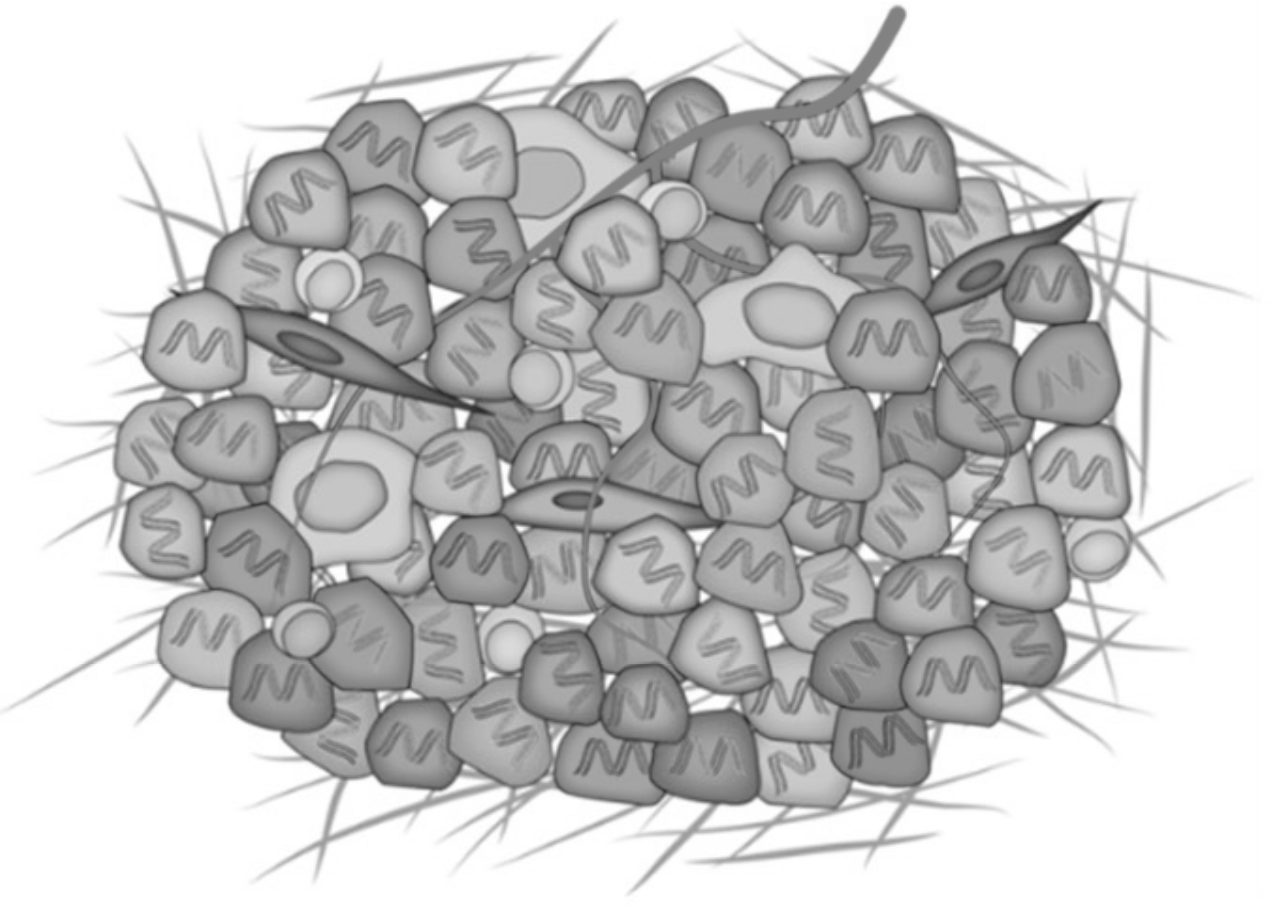
\includegraphics[scale=.8]{images/tumor_heterogenity_bw.png}
      \end{textblock*}
      \begin{textblock*}{5cm}(2.2cm,4.3cm)
        \includegraphics<2,3>[scale=0.05,width=1cm]{images/down_arrow.jpg}
      \end{textblock*}
      \begin{textblock*}{1cm}(0.5cm,5.3cm)
        \includegraphics<2,3>[scale=.8]{images/tumor_heterogenity_color.png}
      \end{textblock*}
    \end{column}

    \begin{column}{0.7\textwidth}
      \begin{overlayarea}{\linewidth}{1\textheight}
        \metroset{block=fill}
        \begin{block}{Por qué}
          \vskip0.5em
          \begin{itemize}
            \item Diferentes poblaciones tumorales.
            \item Micro-entorno tumoral: diferentes tipos \\ celulares con complejas interacciones.
            \item Sello de Identidad del cáncer.
          \end{itemize}
        \end{block}
        \metroset{block=fill}

        \only<2>{\begin{figure}
            \makebox(230,15)[rt]{\includegraphics<2>[height=4cm]{images/tumor_hallmarks_degradado_3.png}}
          \end{figure}}

        \only<3>{\begin{figure}
            \makebox(230,15)[rt]{\includegraphics<3>[height=4cm]{images/tumor_hallmarks_degradado_2.png}}
          \end{figure}}

      \end{overlayarea}
    \end{column}
  \end{columns}
\end{frame}


\begin{frame}[fragile]{Papel del sistema inmune en la enfermedad}
  \Fonteight
  \begin{alertblock}{Papel clave}
    \begin{itemize}
      \item La similitud entre células será máxima cuando sus $k$-vecinos son los
            mismos $\rightarrow$ mismo fenotipo.
      \item Similitud decaerá entre células que compartan menos vecinos conectados
            $\rightarrow$ distinto fenotipo.
    \end{itemize}
  \end{alertblock}

  \begin{alertblock}{Terapias}
    \begin{itemize}
      \item La similitud entre células será máxima cuando sus $k$-vecinos son los
            mismos $\rightarrow$ mismo fenotipo.
      \item Similitud decaerá entre células que compartan menos vecinos conectados
            $\rightarrow$ distinto fenotipo.
    \end{itemize}
  \end{alertblock}

  \begin{figure}
    \centering
    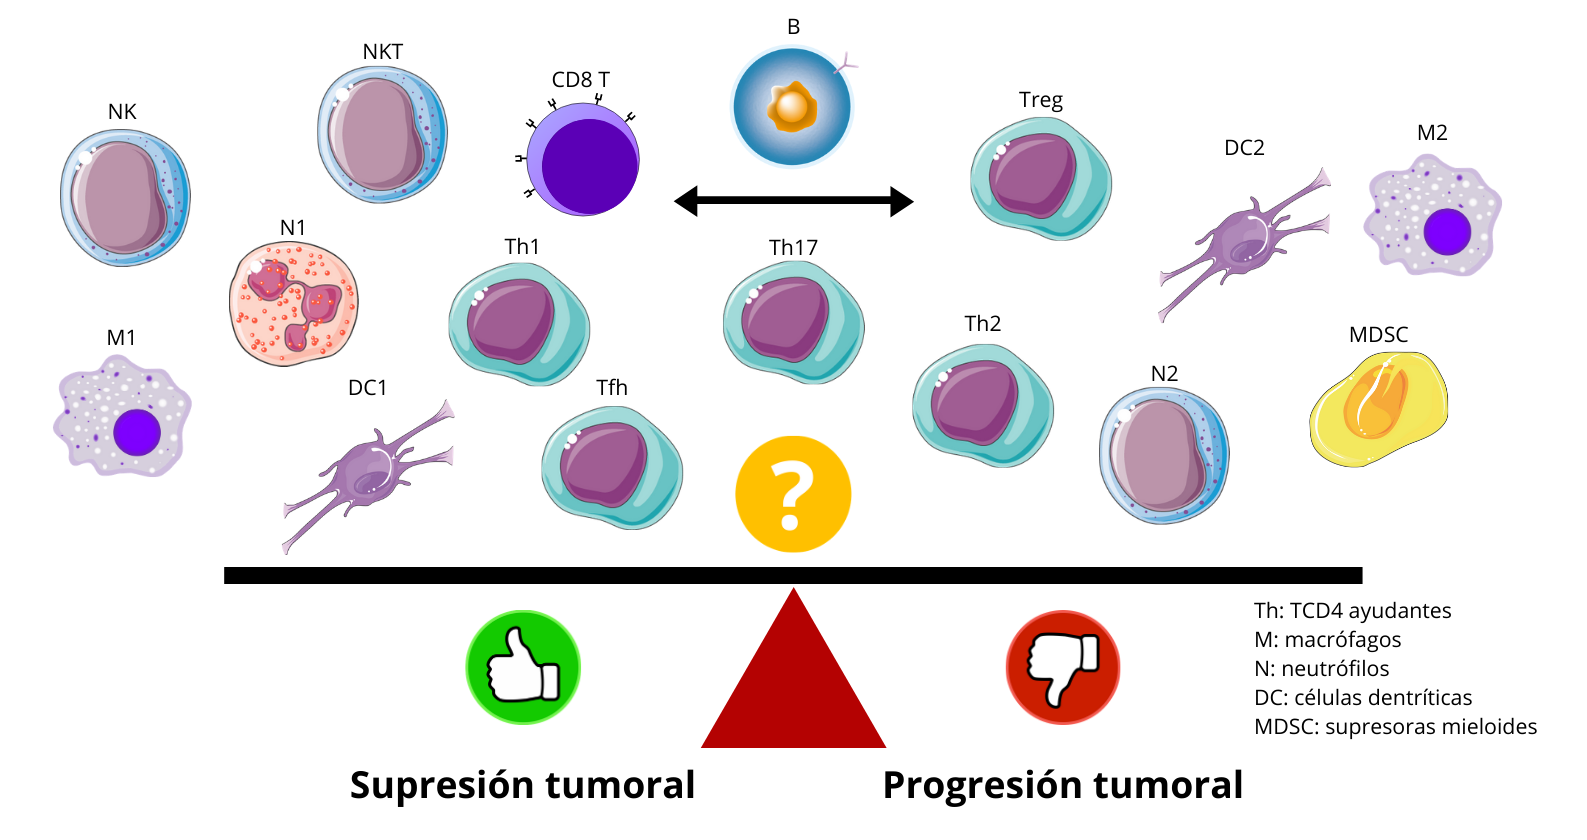
\includegraphics[width=7cm]{images/balance_Imm_2.png}
  \end{figure}

\end{frame}


\begin{frame}[fragile]{Caso de estudio: cáncer de mama}
  \vskip1em
  Enfermedad altamente \alert{\textbf{heterogénea desde el punto de vista molecular}}.
  \Fontvi
  \vskip0.5em
  \begin{columns}
    \begin{column}{0.5\textwidth}
      \vskip-0.5em
      \begin{alertblock}{Subtipos intrínsecos del cáncer}
        \vskip-0.5em
        \Fonteight{
          \begin{itemize}
            \item Luminal A (ER+).
            \item Luminal B (ER+/HER2+).
            \item HER2 enriquecido (HER2+).
            \item Triple negativo (TNBC).
          \end{itemize}
        }
      \end{alertblock}
      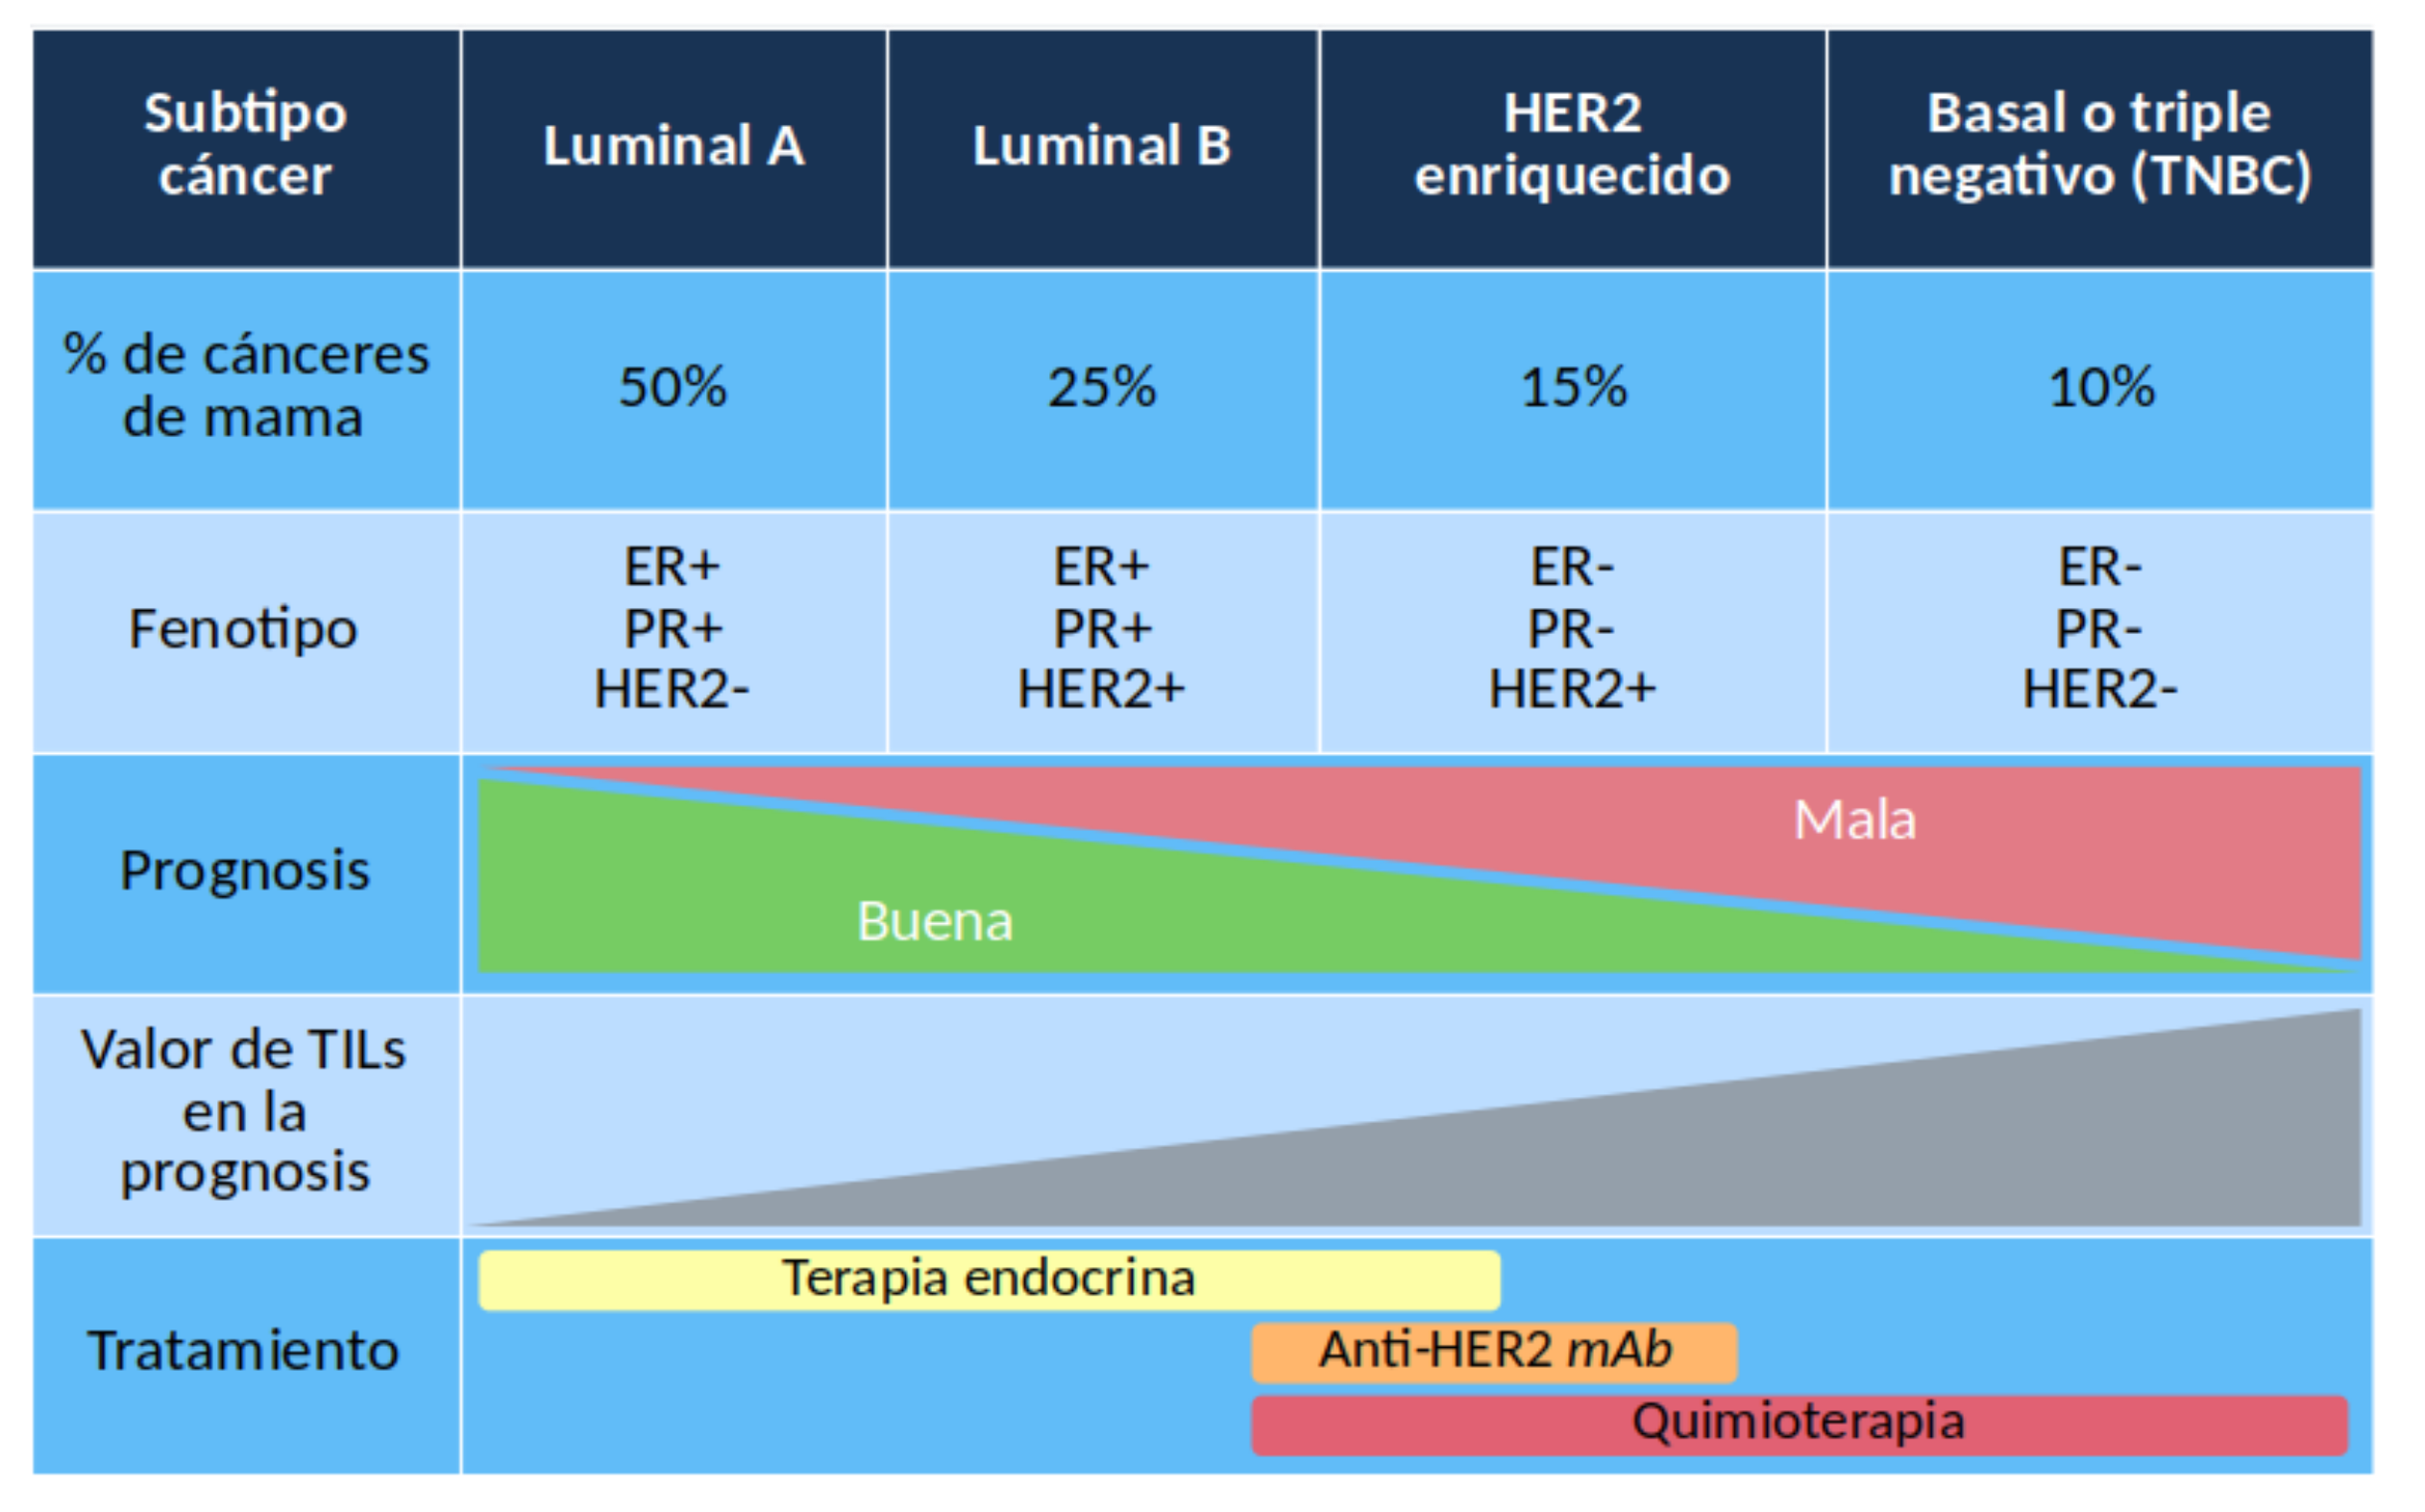
\includegraphics[width=7cm]{images/tabla_breast_2_mod.png}
    \end{column}
    \begin{column}{0.6\textwidth}
      \begin{alertblock}{Importancia de las células inmunes infiltradas}
        \vskip-0.5em
        \Fonteight{
          \begin{itemize}
            \item Luminal A (ER+).
            \item Luminal B (ER+/HER2+).
            \item HER2 enriquecido (HER2+).
            \item Triple negativo (TNBC).
          \end{itemize}
        }
      \end{alertblock}
    \end{column}
  \end{columns}
\end{frame}

% Tecnologías para estudiar células: scRNAseq --------------------------------------

% \subsection{1.2. Tecnologías para explorar la heterogeneidad celular: \textit{scRNA-seq}}

\begin{frame}[fragile,t]{Estudio de la heterogeneidad celular}
  % \vskip0.5em
  Necesidad de métodos para el estudio de la heterogeneidad celular.
  % \Fontvi
  \vskip-0.7em
  % \begin{overlayarea}{\linewidth}{1\textheight}
  \begin{columns}
    \begin{column}{0.65\textwidth}
      \vskip-0.5em
      \begin{alertblock}{Tradicionalmente}
        \vskip1mm
        A nivel de proteína mediante técnicas inmunohistoquímicas, inmunofluorescencencia y citometría de flujo.
      \end{alertblock}
      \begin{alertblock}{Tecnologías de alto rendimiento}
        \vskip1mm
        A nivel transcriptómico mediante NGS: \textit{RNA-seq}.\\
        \vskip1mm
        Dos variantes:
      \end{alertblock}
    \end{column}

    \begin{column}{0.3\textwidth}
      \vskip7mm
      \begin{highlightblock}
        \centering
        \Fontvi{Pequeña combinación de marcadores génicos}
      \end{highlightblock}
      \vskip1mm
      \begin{highlightblock}
        \centering
        \Fontvi{Estatus funcional completo}
      \end{highlightblock}
    \end{column}

  \end{columns}

  \vskip-1.5em

  % Parte inferior
  \begin{columns}
    \begin{column}{0.7\textwidth}
      \Fontvi
      \begin{itemize}
        \item \textit{Bulk RNA-seq} (nivel tisular): los niveles de expresión corresponden al sumatorio de tipos celulares presentes en las muestras.
              \vskip5mm
        \item \textit{Single-cell RNA-seq} (nivel celular): los niveles de expresión corresponden a cada célula individual que compone la muestra.
      \end{itemize}
    \end{column}

    \begin{column}{0.3\textwidth}
      \begin{figure}
        \centering
        \hskip-4mm
        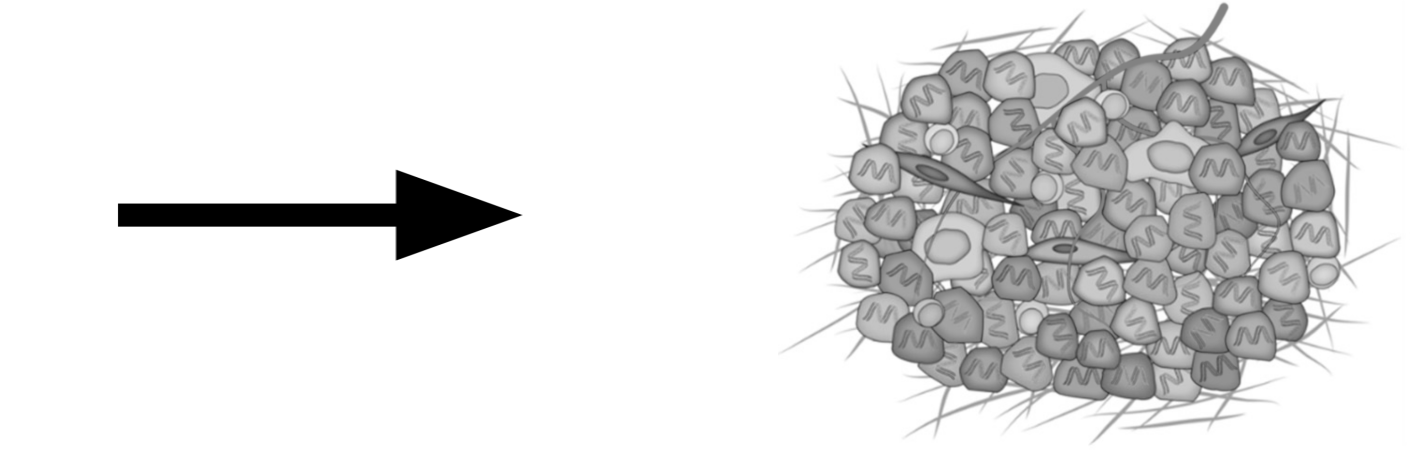
\includegraphics[width=4cm]{images/tumor_bw_arrow.png}\\
        \hskip-4mm
        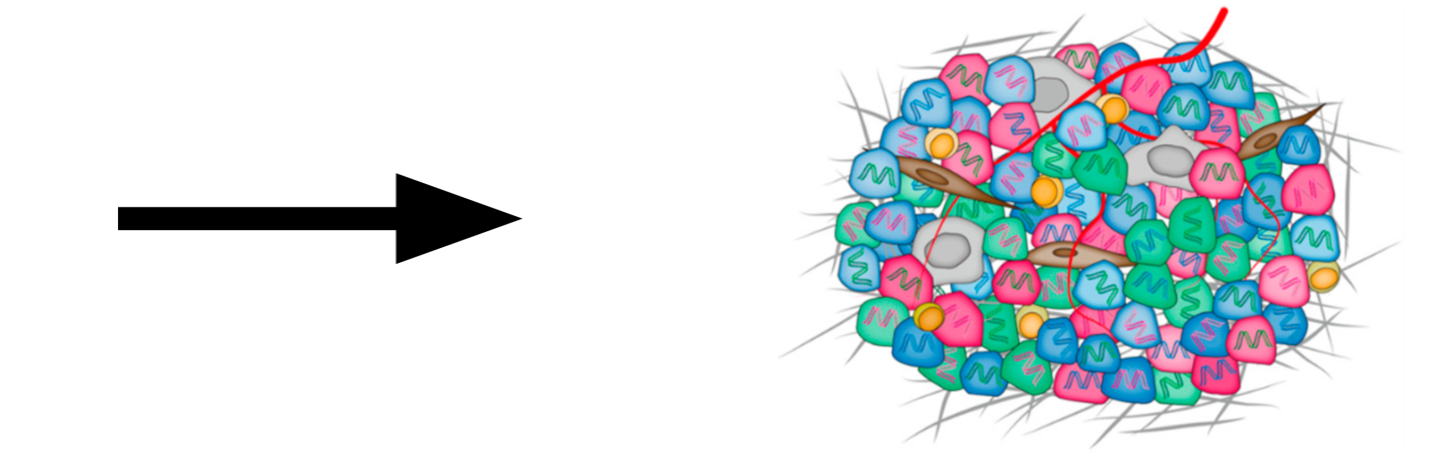
\includegraphics[width=4cm]{images/tumor_color_arrow.png}
      \end{figure}
    \end{column}
  \end{columns}
  % \end{overlayarea}
\end{frame}


\begin{frame}[t]{\textit{scRNA-seq}: Ventajas e inconvenientes}
  % \vskip0.2em
  % \begin{alertblock}{Comunidad}
  %   \vskip0.5mm
  %   Presencia de grupos de nodos que están
  %   más densamente conectados entre sí que con otros nodos.
  % \end{alertblock}
  \vskip-0.7cm
  \begin{columns}[t]
    \begin{column}{0.5\textwidth}
      \begin{alertblock}{Ventajas}
        \begin{itemize}
          \item Estatus funcional de cada célula.
          \item Caracterización de las poblaciones celulares. Potencial identificación de tipos celulares no esperados.
          \item Potencial aplicación traslacional: mejora del diagnóstico, terapias dirigidas, etc.
        \end{itemize}
      \end{alertblock}
    \end{column}
    \begin{column}{0.5\textwidth}
      \begin{alertblock}{Incovenientes}
        \begin{itemize}
          \item Altos costes económicos y protocolos complejos.
          \item No es práctica su aplicación en grandes cohortes de muestras.
          \item Baja eficiencia de captura de ARN.
          \item Mayor ruido técnico.
        \end{itemize}
      \end{alertblock}
    \end{column}
  \end{columns}
  \vskip0.5em
  \only<2,3,4>{\begin{beamercolorbox}[sep=0.2cm]{coloredboxstuff}
      \textbf{ Resultado:} \hspace{1.9cm}\textit{Bulk RNA-seq} sigue siendo el estándar. \hspace{\fill}
    \end{beamercolorbox}}
  \only<3,4>{\begin{beamercolorbox}[sep=0.2cm,center]{coloredboxstuff}
      \textbf{Problema:} No tiene en cuenta en qué proporción contribuye cada tipo celular a los niveles de expresión medidos.
    \end{beamercolorbox}}
  \only<4>{\begin{beamercolorbox}[sep=0.2cm,center]{coloredboxstuff}
      \textbf{Necesidad:} Métodos computacionales que permitan estimar las proporciones de cada tipo celular medidas en muestras \textit{bulk RNA-seq}.
    \end{beamercolorbox}}
\end{frame}

% \subsection{1.3. Métodos de deconvolución de muestras \textit{bulk RNA-seq}}

\begin{frame}{Deconvolución de muestras \textit{bulk RNA-seq}}
  \alert{Deconvolución:} estimación de la señal individual de cada uno de los componentes (tipos celulares) a partir de una mezcla de los mismos (muestra tisular).
  \begin{itemize}
    \item Sustituto de experimentos \textit{scRNA-seq} por sus altos costes económicos o la imposibilidad de su aplicación.
    \item Control de la contribución de cada tipo celular a las muestras tisulares $\rightarrow$ evitar factores de confusión en análisis de expresión diferencial.
  \end{itemize}
  % \vskip-0.5em
  \begin{figure}
    \centering
    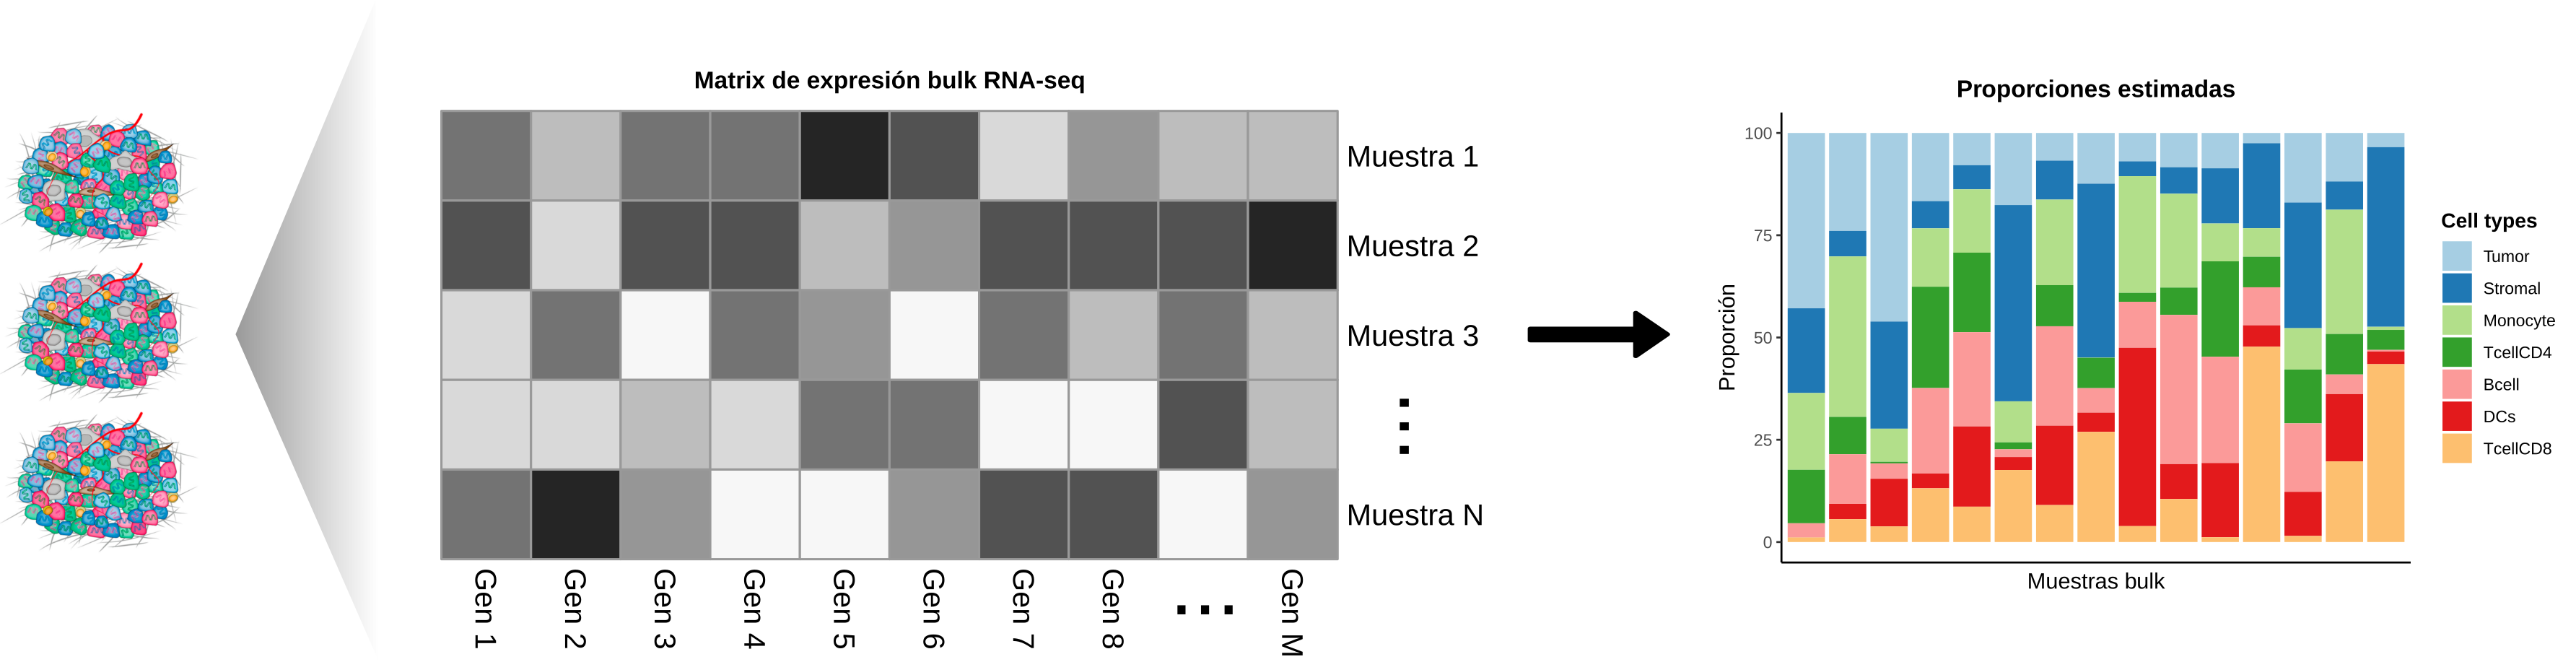
\includegraphics[width=14cm]{images/deconvolution_workflow.png}
  \end{figure}
\end{frame}


\begin{frame}{Deconvolución: marco de trabajo}
  \begin{overlayarea}{\linewidth}{1\textheight}
    % \vskip-1em

    \only<1>{
      \vskip0.7mm
      \hspace{-1mm}
      \begin{equation*}
        T_{ij} = \sum_{k=1}^K C_{ik} \cdot P_{kj} + e_{ij}
      \end{equation*}
    }
    \only<2>{
      \vskip0.15mm
      \centering
      \hspace{-4mm}
      \includegraphics[scale=0.135]{images/ecuación01_mod_def_def_1.png}
    }
    \only<3>{
      \vskip0.15mm
      \centering
      \hspace{-5.2mm}
      \includegraphics[scale=0.135]{images/ecuación01_mod_def_def_2.png}
    }
    \only<4>{
      \vskip0.15mm
      \centering
      \hspace{-6.4mm}
      \includegraphics[scale=0.135]{images/ecuación01_mod_def_def_3.png}
    }
    \vskip3mm
    \begin{columns}
      \begin{column}{0.5\textwidth}
        \only<1>{
          \vskip2.25mm
          \centering
          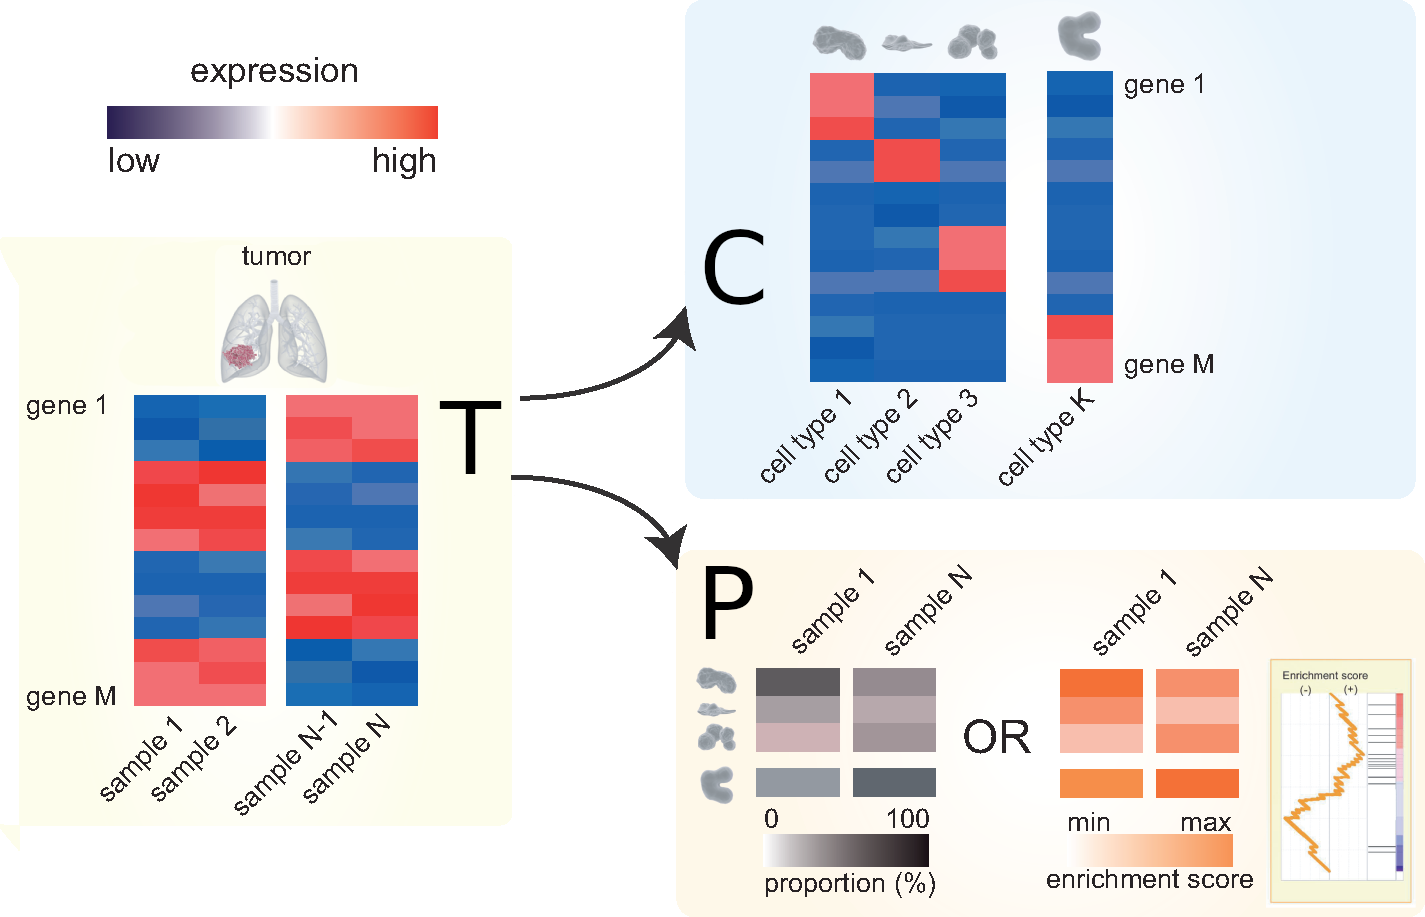
\includegraphics[width=8.5cm]{images/figure4.png}
        }
        \only<2>{
          \vskip-1em
          \centering
          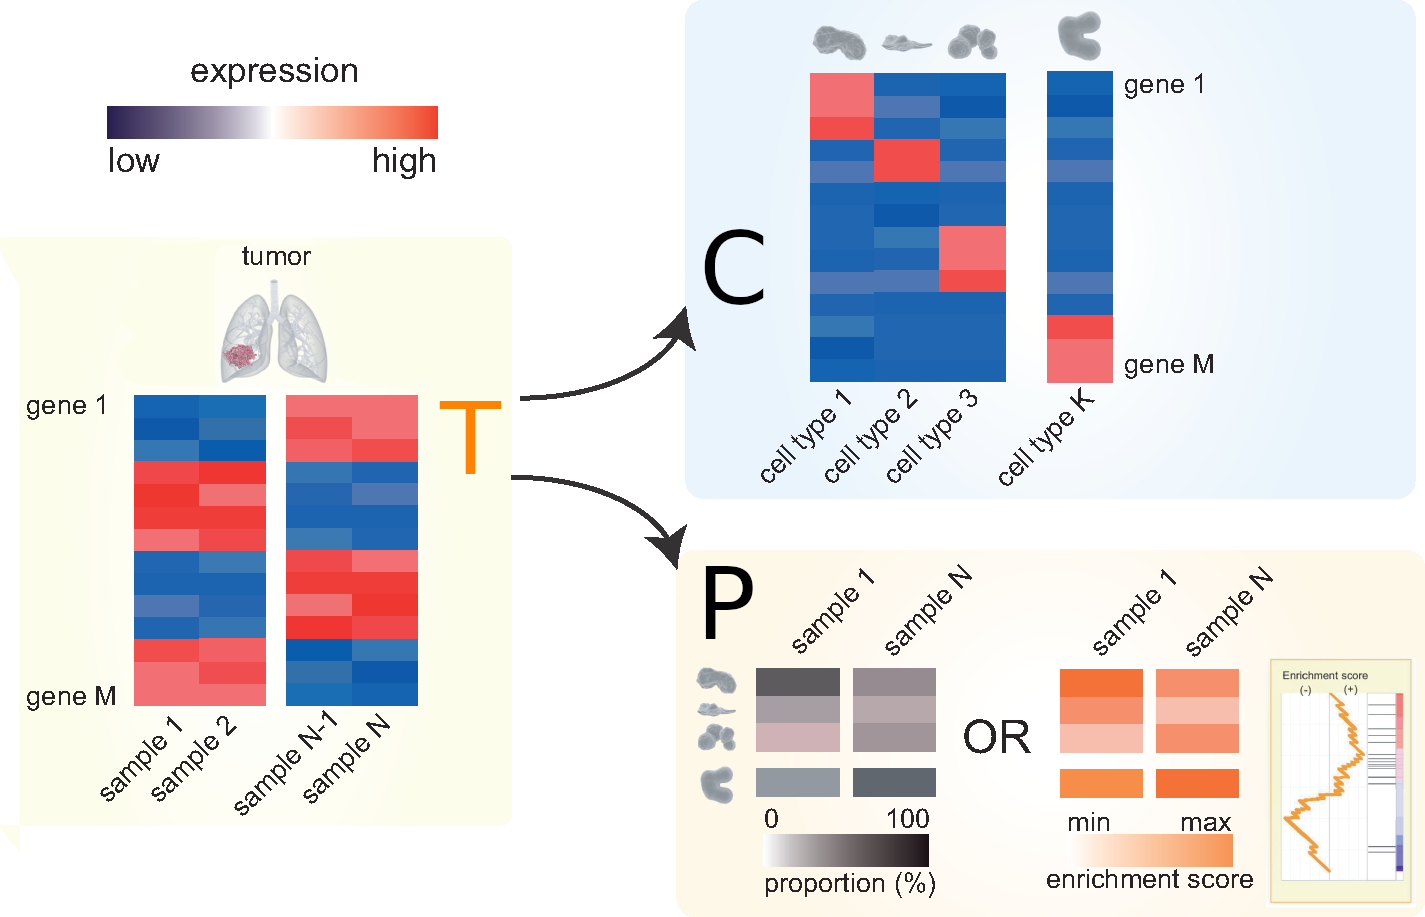
\includegraphics[width=8.5cm]{images/expression_deconv_1.png}
        }
        \only<3>{
          \vskip-1em
          \centering
          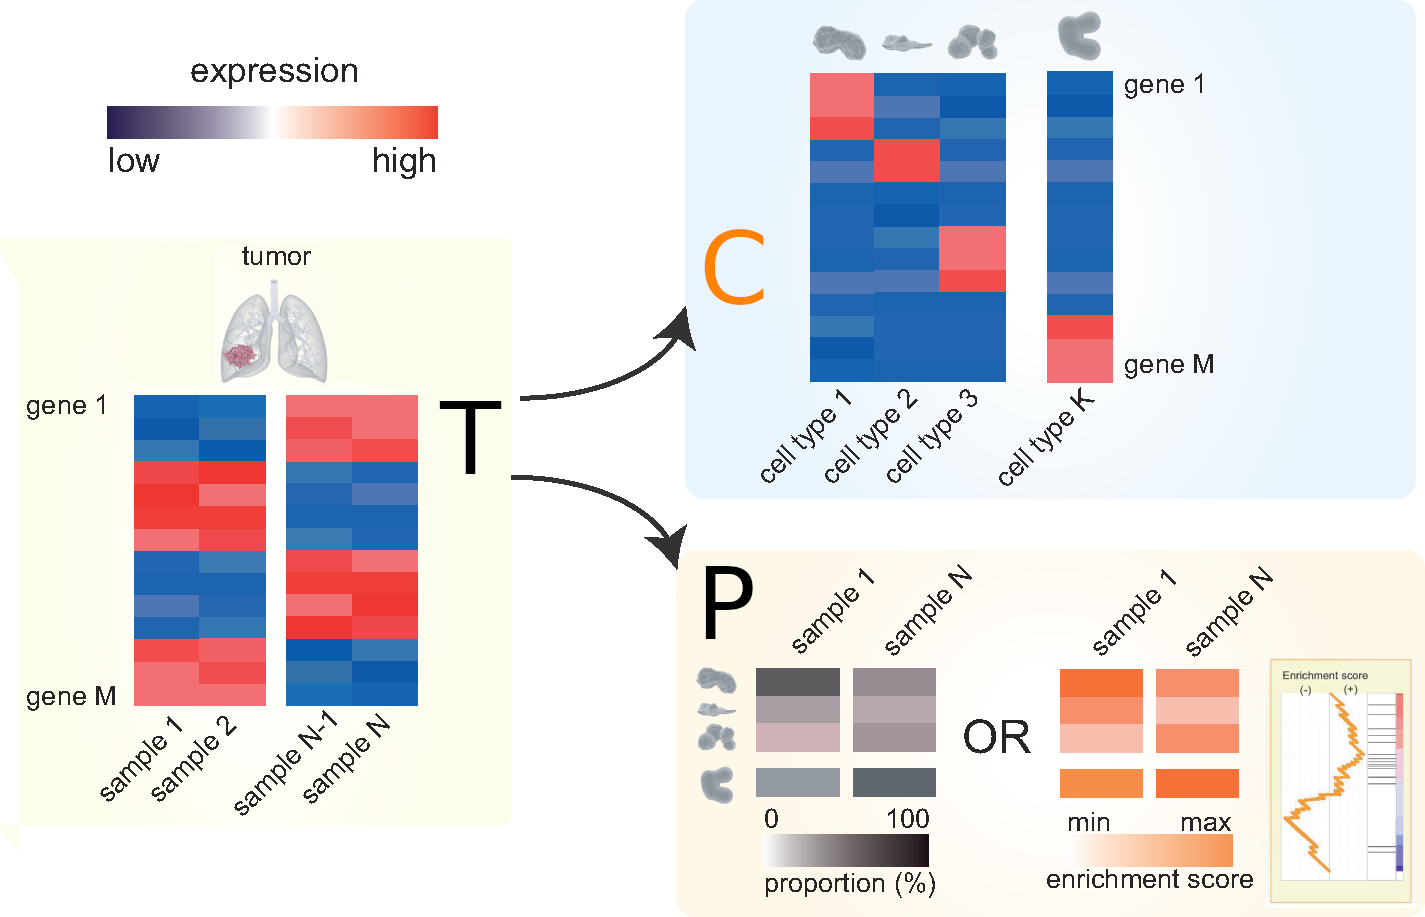
\includegraphics[width=8.5cm]{images/expression_deconv_2.png}
        }
        \only<4>{
          \vskip-1em
          \centering
          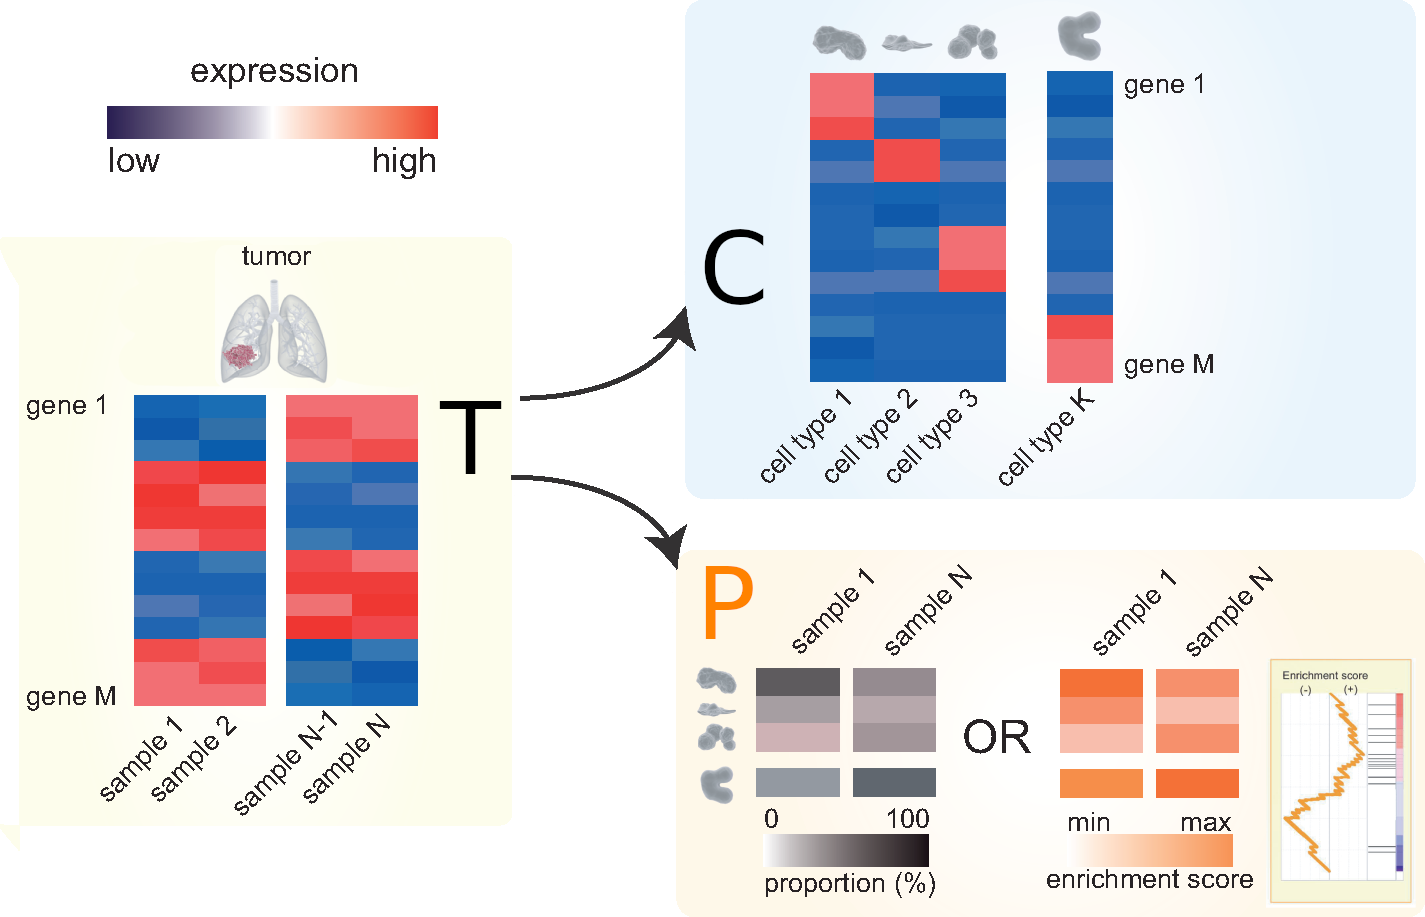
\includegraphics[width=8.5cm]{images/expression_deconv_3.png}
        }
      \end{column}

      \begin{column}{0.4\textwidth}
        \begin{textblock*}{6cm}(10cm,3.5cm)
          \begin{itemize}
            \item $i$: genes ($i = 1...M$).
            \item $j$: muestras \textit{bulk} ($j = 1...N$).
            \item $k$: tipos celulares ($k = 1...K$).
          \end{itemize}
        \end{textblock*}

        \only<4>{
          \begin{textblock*}{6cm}(10cm,5.5cm)
            \begin{alertblock}{Herramientas publicadas}
              \begin{itemize}
                \item Enriquecimiento de sets de genes.
                \item Mínimos cuadrados ordinarios.
                \item $\upsilon$-SVR
              \end{itemize}
            \end{alertblock}
          \end{textblock*}
        }
      \end{column}
    \end{columns}

  \end{overlayarea}
\end{frame}

\begin{frame}[fragile]{Método de deconvolución digitalDLSorter}
  \begin{alertblock}{Características}
    \begin{itemize}
      \item Método basado en \alert{Aprendizaje Profundo} $\rightarrow$ revolución en el campo del Aprendizaje Automático durante los últimos años por su desempeño.
      \item Uso de datos \alert{\textit{scRNA-seq}} $\rightarrow$ perfiles de expresión procedentes del propio entorno de estudio (micro-entorno tumoral cáncer de mama, cáncer de colon, entorno neuronal, etc.).
    \end{itemize}
  \end{alertblock}

  \begin{alertblock}{Implementación}
    \begin{itemize}
      \item \textit{Pipeline} escrita en varios lenguajes de programación.
      \item Cada paso escribe los datos intermedios en disco como ficheros tabulados.
      \item No ofrece la opción de utilizar modelos preentrenados.
      \item Uso complicado por otros usuarios.
    \end{itemize}
  \end{alertblock}
\end{frame}


%--------------------------------------------------------------------------%

%%%%%%%%%%%%%%%%%%%%%%%%%%%%%%%%%%%%%%%%%%%%%%%%%%%%%%%%%%%%%%%%%%%%%%%%%%%%%%%%%%%%
%%%%%%%%%%%%%%%%%%%%%%%%%%%%%%%%%%% OBJETIVOS %%%%%%%%%%%%%%%%%%%%%%%%%%%%%%%%%%%%%%
%%%%%%%%%%%%%%%%%%%%%%%%%%%%%%%%%%%%%%%%%%%%%%%%%%%%%%%%%%%%%%%%%%%%%%%%%%%%%%%%%%%%

\section[Objetivos]{Objetivos}

\begin{frame}{Objetivos}
  % \metroset{block=fill}
  % \vskip-1em
  % \begin{alertblock}{Objetivos}
  %   \vskip0.20em
  %   Grafo ponderado con pesos basados en el número de vecinos que comparten.
  % \end{alertblock}
  \begin{enumerate}[<alert@+>]
    \item Transformación de la \textit{pipeline} original en un paquete de R.
          \begin{itemize}
            \item Unificación de los lenguajes de programación $\rightarrow$ R.
            \item Evitar la lectura/escritura de ficheros tabulados en disco.
            \item Funcionalidades nuevas $\rightarrow$ uso de ficheros HDF5 como \textit{back-end}, implementación de parámetros para construir modelos más personalizados.
            \item Generación de documentación y viñeta $\rightarrow$ facilitar su uso.
          \end{itemize}
    \item Análisis de datos \textit{scRNA-seq} procedentes de cáncer de mama.
          \begin{itemize}
            \item Separación tipos tumorales y no tumorales.
            \item Identificación de tipos celulares no tumorales.
          \end{itemize}
    \item Aplicación de la herramienta implementada.
          \begin{itemize}
            \item Construcción de varios modelos y comparativa.
            \item Incorporación de los mejores como modelos preentrenados en el paquete.
          \end{itemize}
  \end{enumerate}

\end{frame}

%%%%%%%%%%%%%%%%%%%%%%%%%%%%%%%%%%%%%%%%%%%%%%%%%%%%%%%%%%%%%%%%%%%%%%%%%%%%%%%%%%%%
%%%%%%%%%%%%%%%%%%%%%%%%%%%%%%%%%%%%% PAQUETE R %%%%%%%%%%%%%%%%%%%%%%%%%%%%%%%%%%%%
%%%%%%%%%%%%%%%%%%%%%%%%%%%%%%%%%%%%%%%%%%%%%%%%%%%%%%%%%%%%%%%%%%%%%%%%%%%%%%%%%%%%

\section[digitalDLSorteR: transformación de la \textit{pipeline} en paquete de R]{digitalDLSorteR: transformación de la \textit{pipeline} en paquete de R}

% Fundamento -----------------------------------------------------------------

% \subsection{2.1. Fundamento del método}

\begin{frame}[fragile]{Fundamento del método}
  \begin{overlayarea}{\linewidth}{1\textheight}
    \only<1>{
      \centering
      \vskip1em
      \hspace{-2.8mm}
      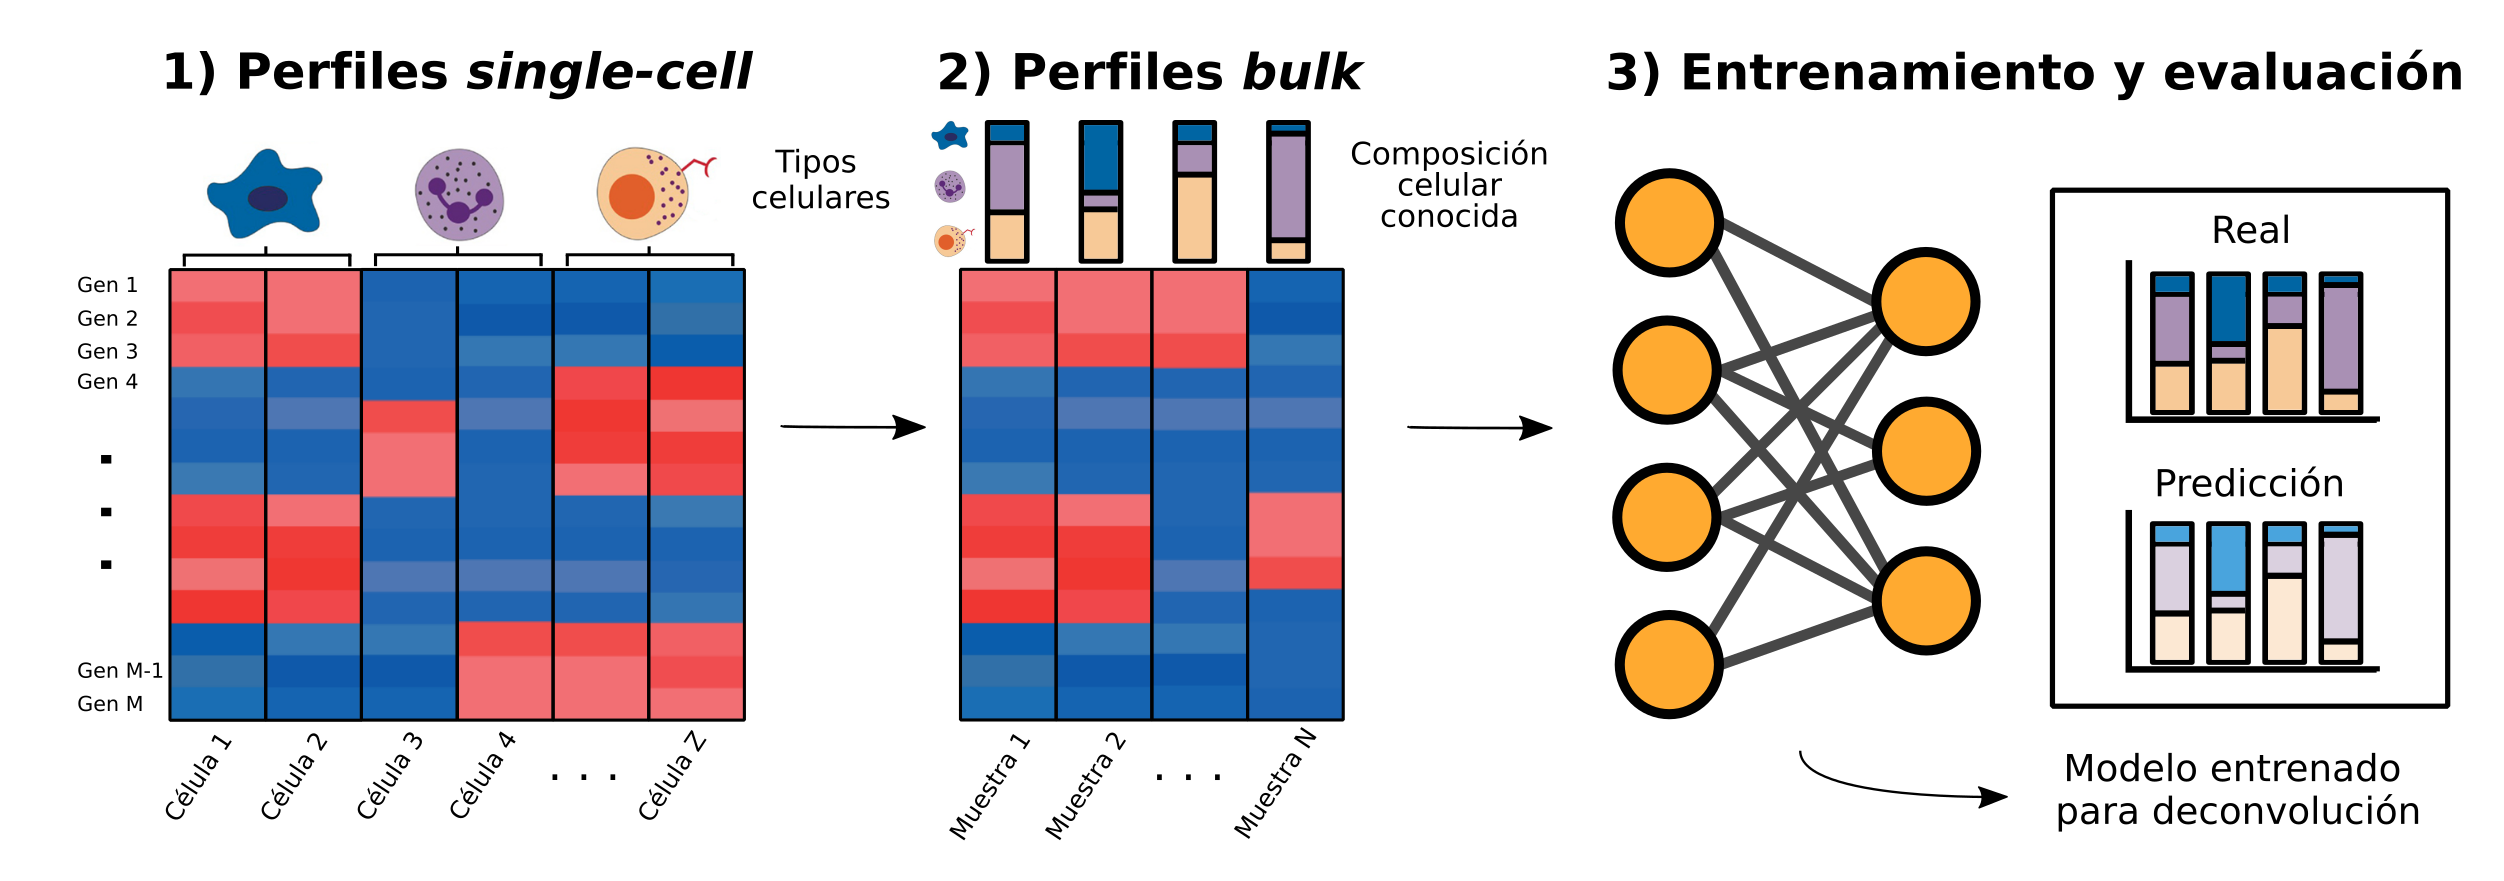
\includegraphics[width=10cm]{images/fund_model_0.png}
    }
    \only<2>{
      \centering
      \vskip1em
      \hspace{-4mm}
      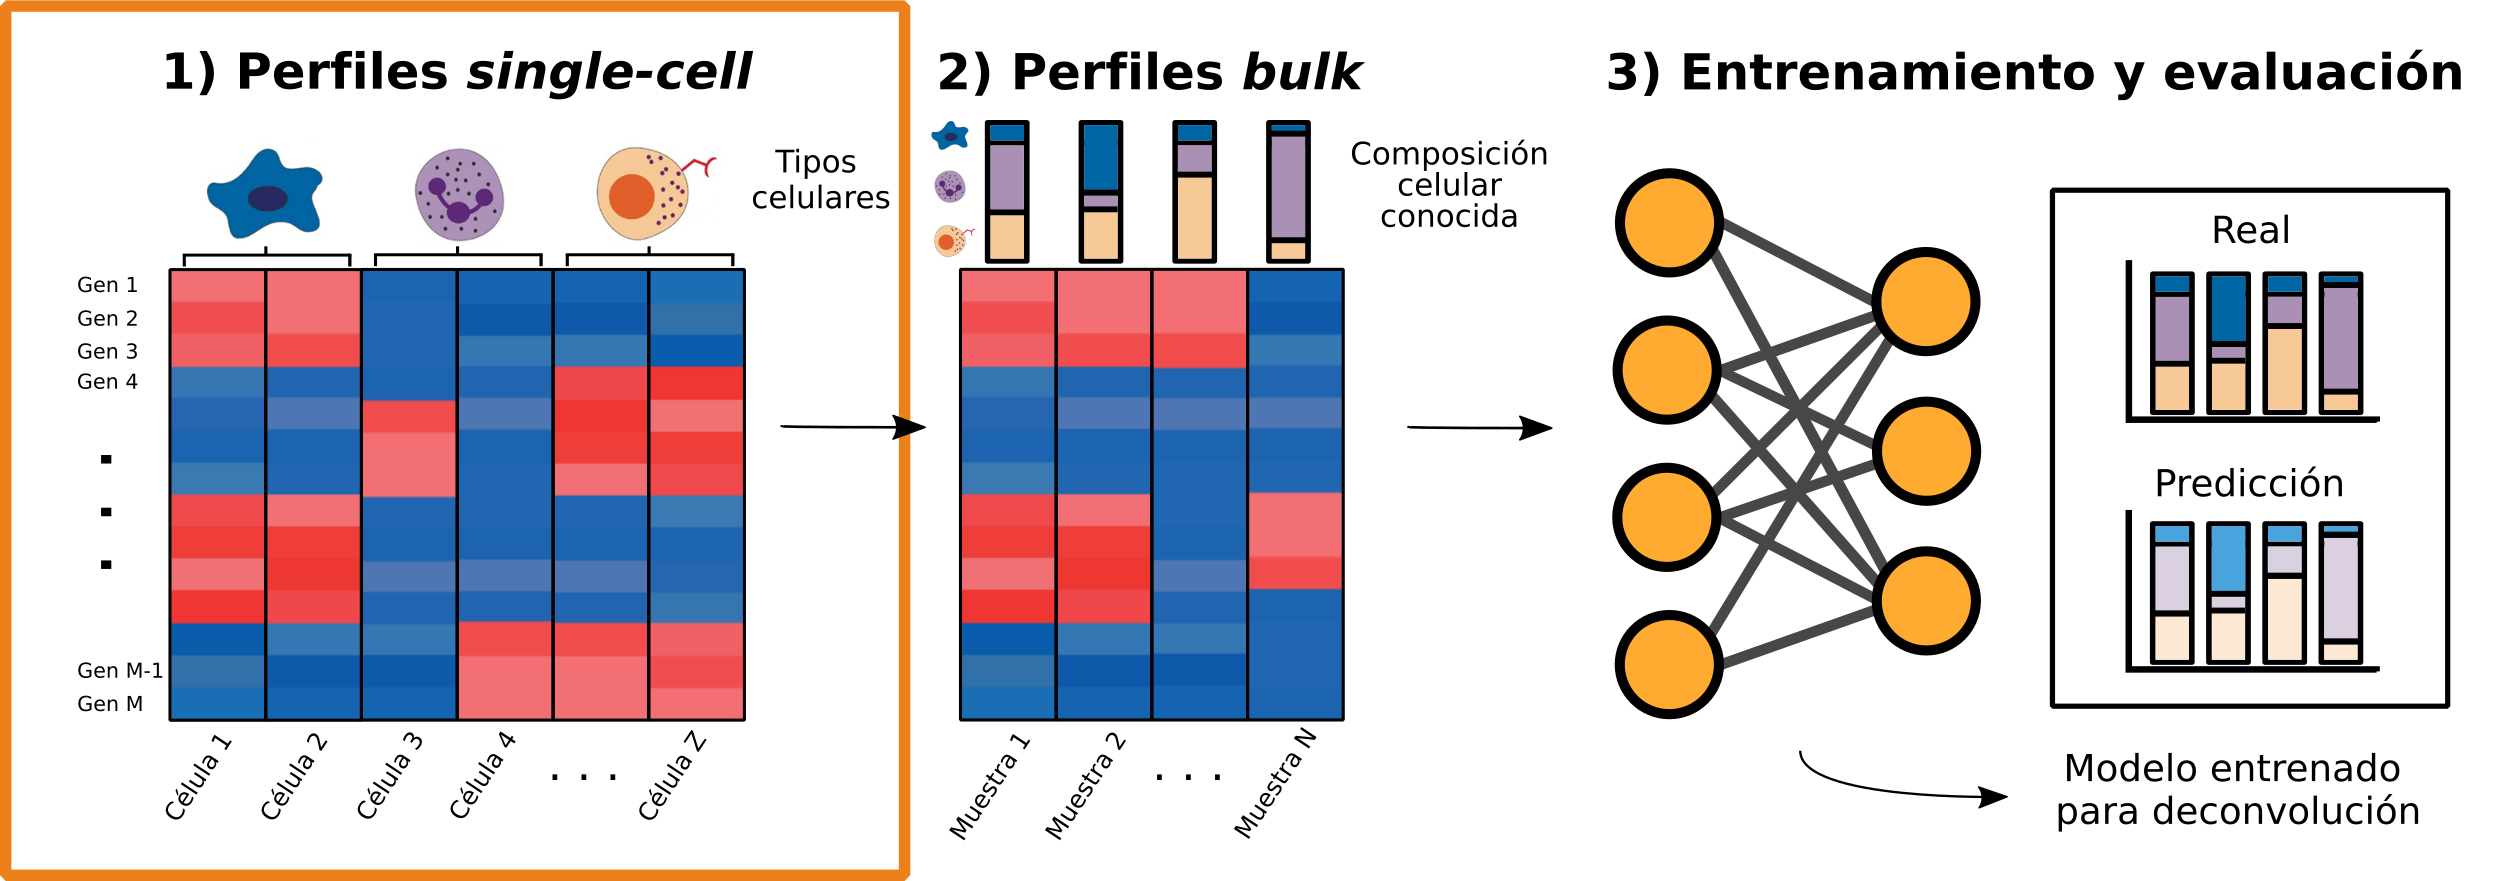
\includegraphics[width=10cm]{images/fund_model_1.png}
    }
    \only<3>{
      \centering
      \vskip1em
      \hspace{-5.2mm}
      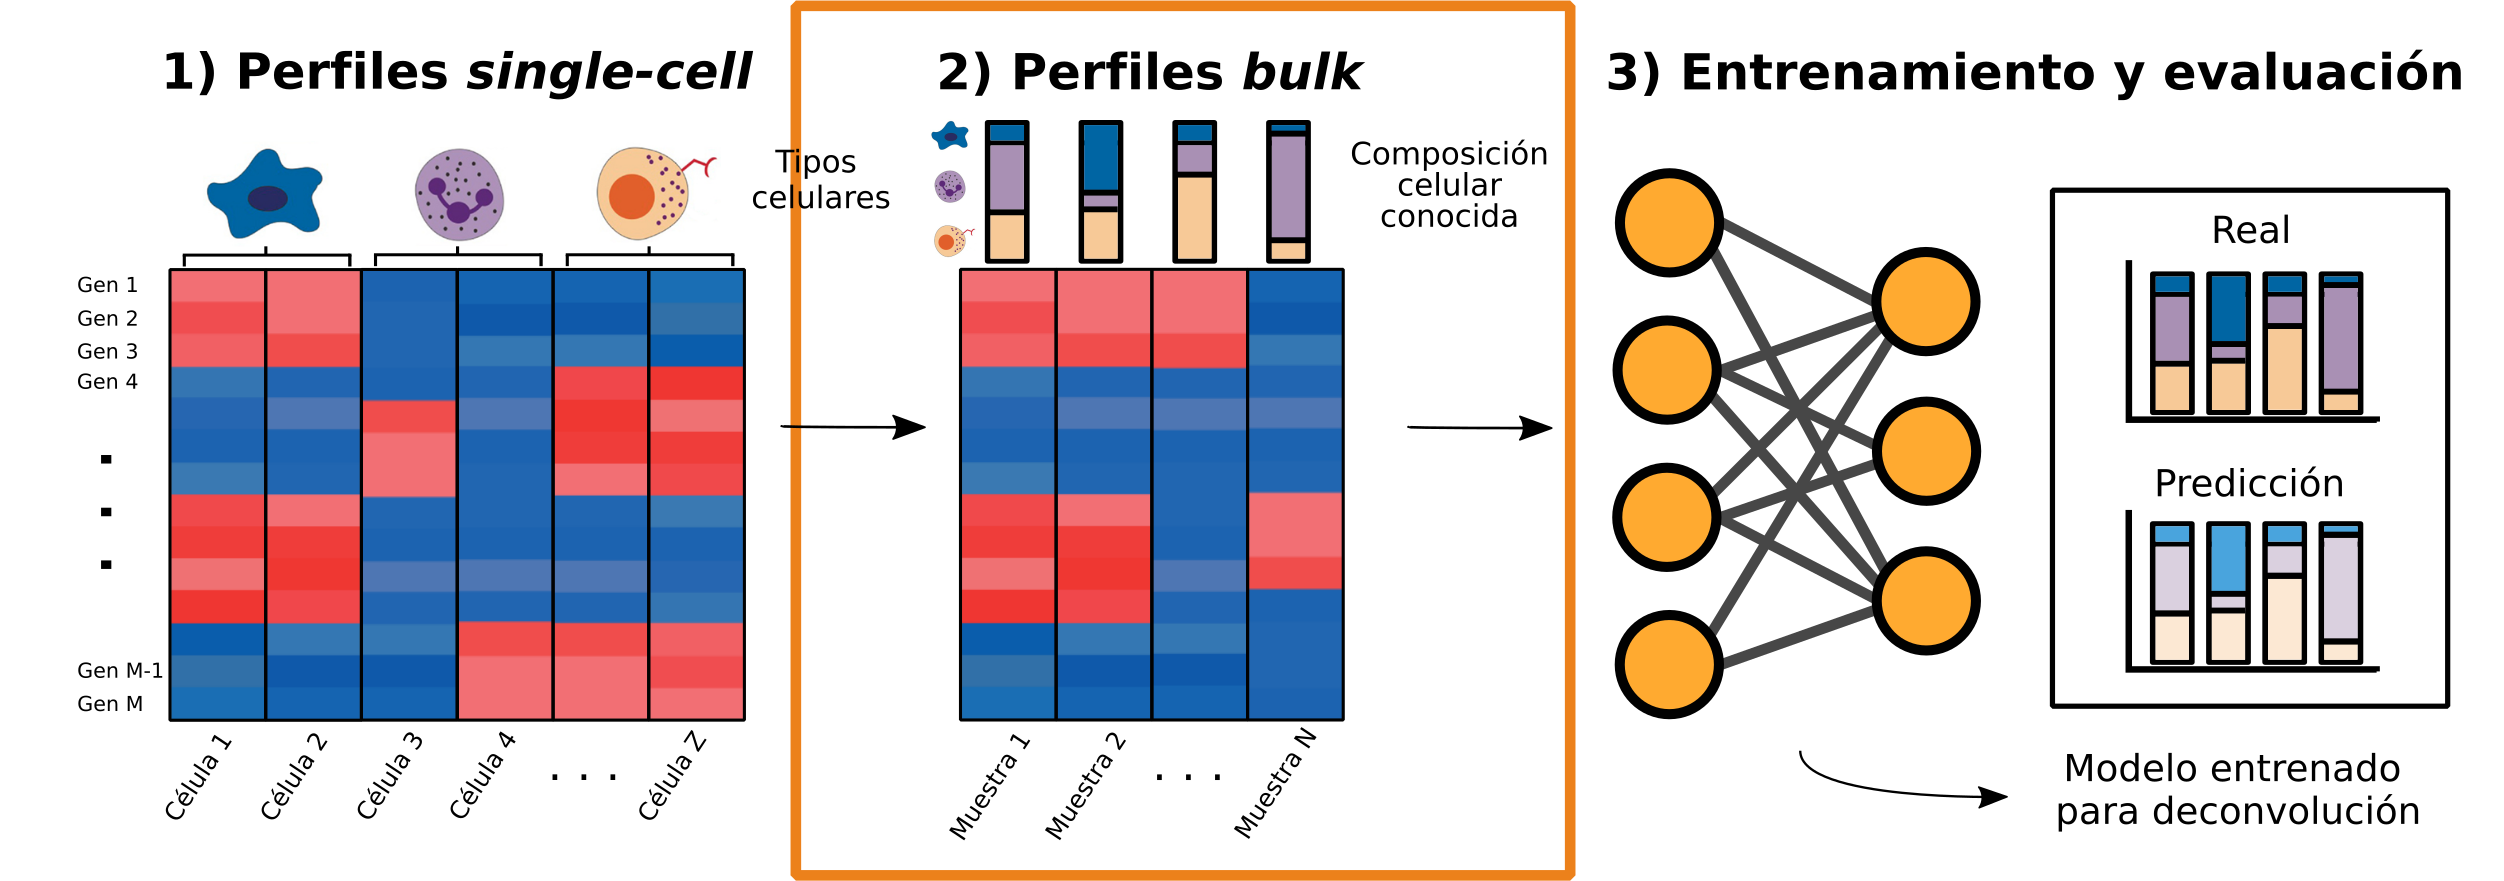
\includegraphics[width=10cm]{images/fund_model_2.png}
    }
    \only<4>{
      \centering
      \vskip1em
      \hspace{-6.4mm}
      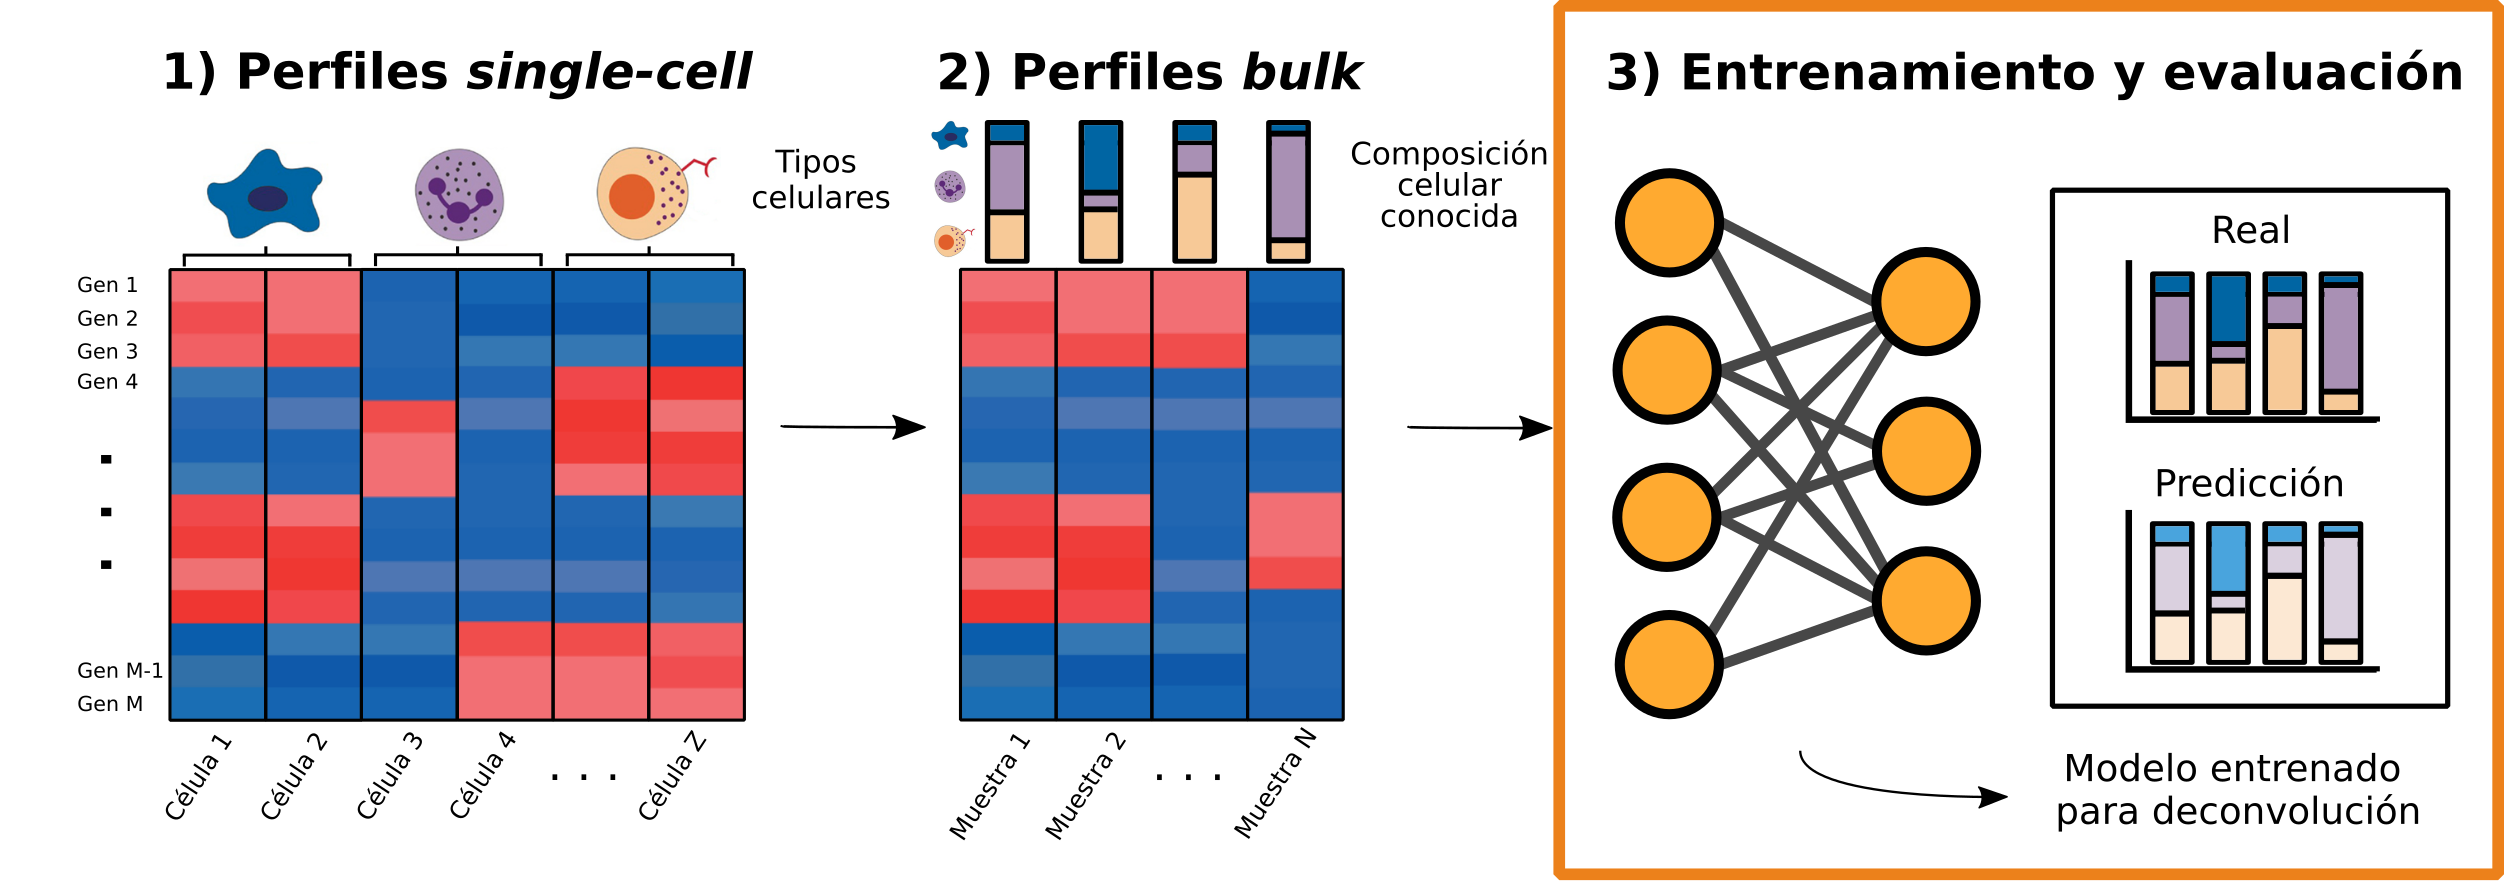
\includegraphics[width=10cm]{images/fund_model_3.png}
    }

    \only<5>{
      \centering
      \vskip1em
      \includegraphics[scale=0.2]{images/ecuación01_mod_def_def_3.png}
      \vskip1.55em
    }

    \begin{enumerate}
      \alert<2>{\item Simulación de perfiles \textit{scRNA-seq} (si es necesario):} uso del modelo ZINB-WaVE en caso de tipos celulares poco representados o pocas células de partida.
            \alert<3>{\item Simulación de perfiles \textit{bulk RNA-seq} de composición celular conocida:} agregación de perfiles \textit{single-cell} en función del tipo celular al que pertenecen.
            \alert<4>{\item Entrenamiento y evaluación de la Red Neuronal Profunda:} deconvolución de nuevas muestras \textit{bulk}.
    \end{enumerate}
  \end{overlayarea}
\end{frame}

% Herramienta -----------------------------------------------------------------

% \subsection{2.1. digitalDLSorteR: flujo de trabajo}

\begin{frame}{digitalDLSorteR: flujo de trabajo}

  \begin{alertblock}{Objetivo del método como paquete}
    \begin{enumerate}
      \item Permitir la deconvolución directa de muestras \textit{bulk RNA-seq}.
      \item Permitir la construcción de nuevos modelos a partir de datos \textit{scRNA-seq}
    \end{enumerate}
  \end{alertblock}

  \begin{center}
    \begin{tikzpicture}[sibling distance=5.5cm, level distance=2cm,
        edge from parent/.style={draw,Orange,ultra thick},
        every node/.style = {align=center}]]
      \node[draw=none,fill=none] {\Large{\alert{\textbf{digitalDLSorteR ofrece }}} \\ \Large{\alert{\textbf{dos flujos de trabajo}}}}
      child { node {1. Uso de modelos preentrenados\\integrados en el paquete} }
      child { node {2. Construcción de nuevos modelos\\a partir de \textit{scRNA-seq}} };
    \end{tikzpicture}
  \end{center}
\end{frame}


% Modelos preentrenados ----------------------------------------------------------
% \hbox{\hspace{-0.5em}
\begin{frame}[fragile]
  \frametitle{Uso de modelos preentrenados}
  \begin{figure}
    \centering
    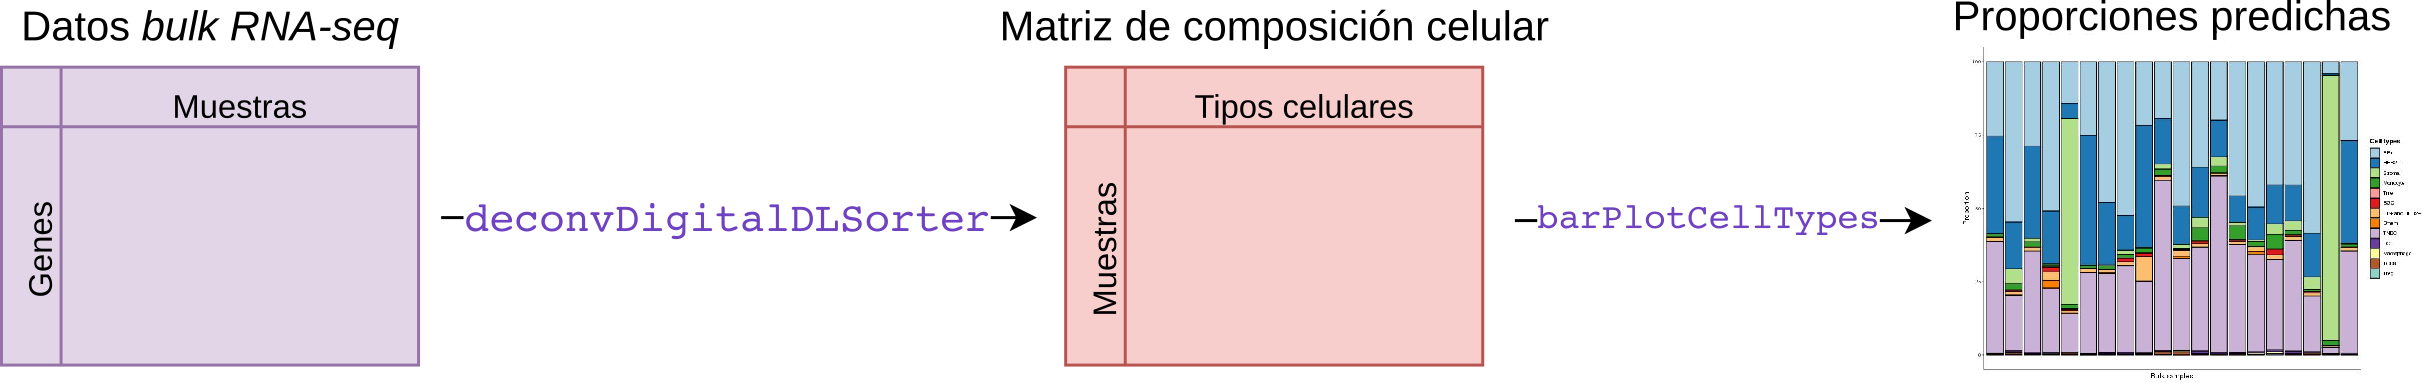
\includegraphics[width=13cm]{images/modelo_preentrenado_3.png}
  \end{figure}

  \begin{columns}
    \begin{column}{0.45\textwidth}
      \lstinputlisting[]{./boxcodes/boxcode1.R}
    \end{column}

    \begin{column}{0.6\textwidth}
      \begin{itemize}
        \item Modelos para la cuantificación de células inmunes en cáncer de mama.
              \begin{enumerate}
                \item Modelo genérico: 7 tipos celulares.
                \item Modelo específico: 13 tipos celulares.
              \end{enumerate}
        \item Datos procedentes de Chung et al., 2017 (\href{https://www.ncbi.nlm.nih.gov/geo/query/acc.cgi?acc=GSE75688}{GSE75688}).
        \item Agregación de tipos celulares con \texttt{simplify.set} y \texttt{simplify.majority}.
      \end{itemize}
    \end{column}
  \end{columns}
\end{frame}


% Construcción de nuevos modelos --------------------------------------------------

\begin{frame}{Construcción de nuevos modelos}
  \begin{alertblock}{Clases}
    \begin{itemize}
      \item \textit{DigitalDLSorter}: núcleo del paquete.
      \item \textit{ProbMatrixCellTypes}: información relativa a las matrices de composición celular.
      \item \textit{DigitalDLSorterDNN}: información relativa a la Red Neuronal Profunda.
      \item Otras clases: \textit{SingleCellExperiment}, \textit{SummarizedExperiment}, etc.
    \end{itemize}
  \end{alertblock}

  \begin{alertblock}{Flujo de trabajo}
    \begin{enumerate}
      \item Carga de datos y simulación de nuevos perfiles \textit{single-cell} (si es necesario).
      \item Generación de la matriz de composición celular.
      \item Simulación de perfiles \textit{bulk RNA-seq} de acuerdo a las proporciones establecidas en el paso anterior. Preparación de los datos para el entrenamiento.
      \item Entrenamiento de la red neuronal y evaluación.
      \item Carga de nuevos datos \textit{bulk} y su deconvolución.
    \end{enumerate}
  \end{alertblock}
\end{frame}

% Carga de datos y simulación de perfiles single-cell -------------------------------

\begin{frame}[fragile]
  \frametitle{1. Carga de datos y simulación de perfiles \textit{single-cell}}

  \begin{figure}
    \centering
    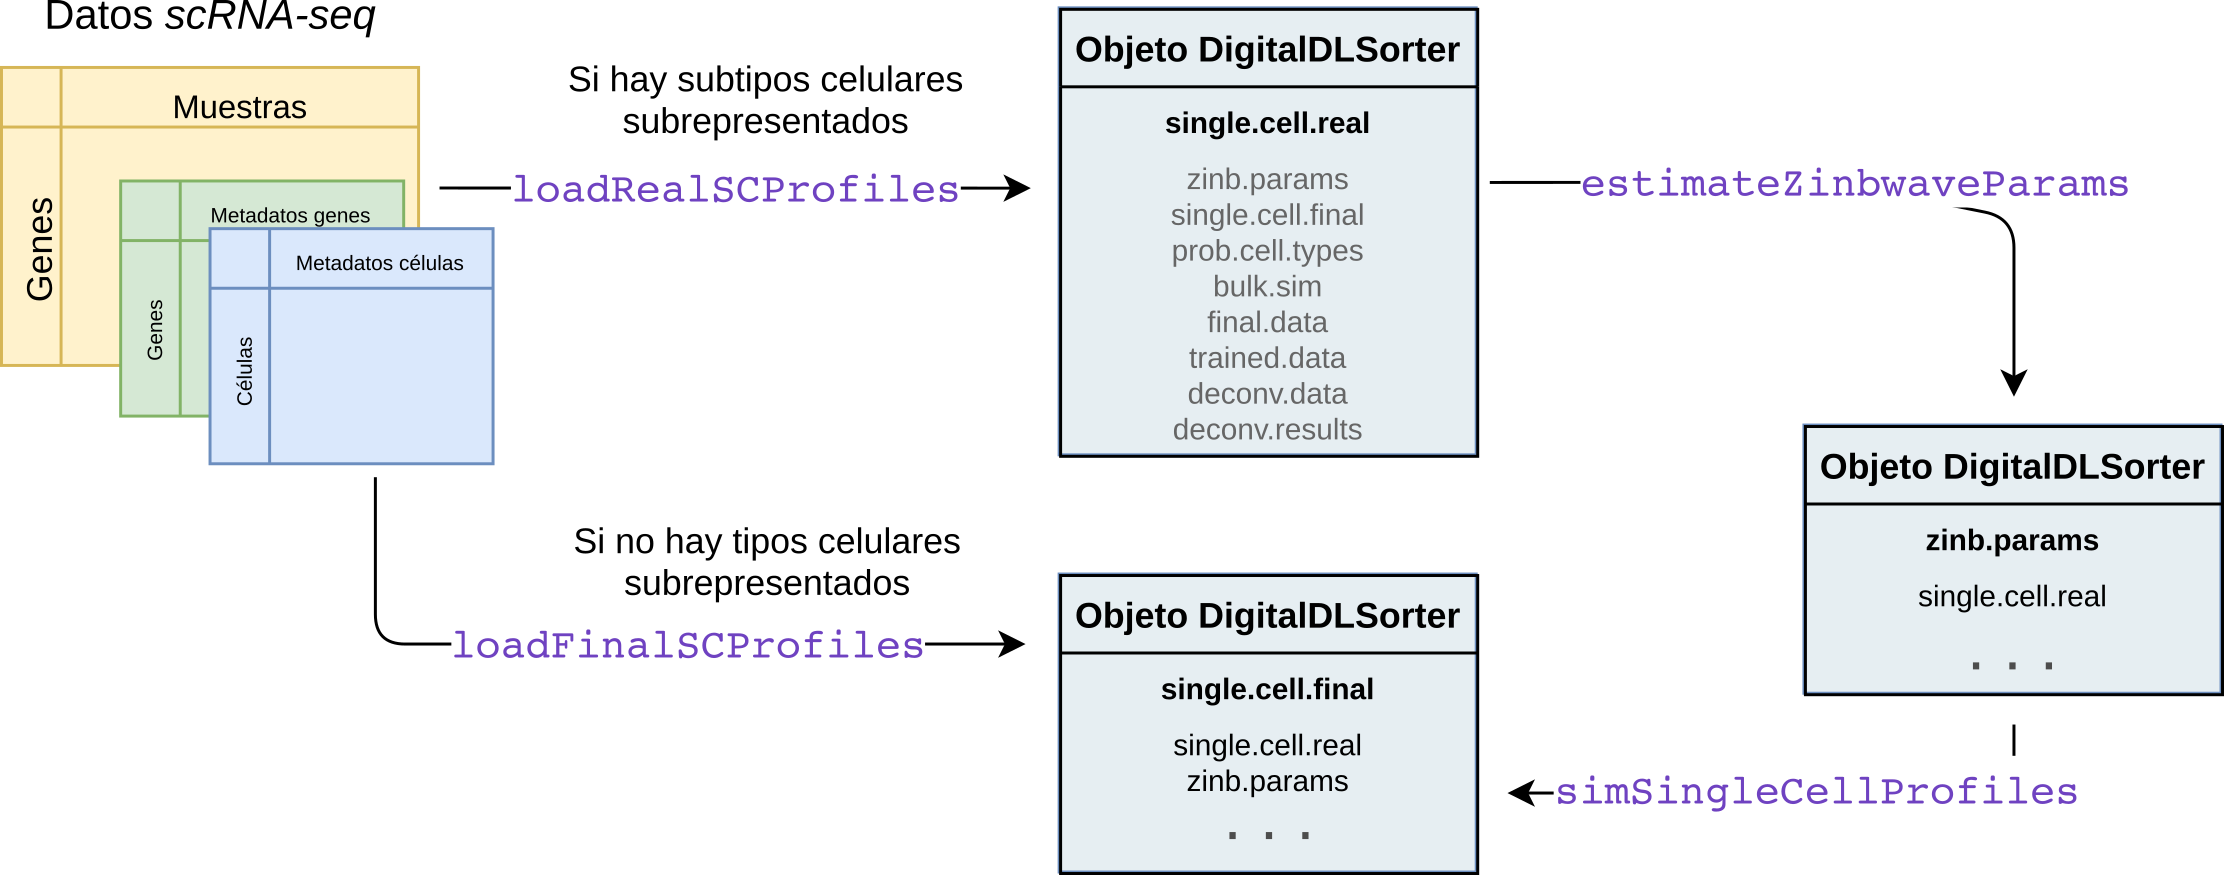
\includegraphics[width=11cm]{images/load_data_1.png}
  \end{figure}

  \begin{itemize}
    \item Carga de los datos en un objeto de la clase \textit{DigitalDLSorter} en el slot \textit{single.cell.real} o \textit{single.cell.final} $\rightarrow$ matriz de expresión, metadatos de células y metadatos de genes.
    \item Si es necesario: estimación de parámetros mediante el modelo ZINB-WaVE y simulación de nuevos perfiles \textit{single-cell}: distribución binomial negativa cero inflada.
  \end{itemize}
\end{frame}

\begin{frame}[fragile,t]{1. Carga de datos y simulación de perfiles \textit{single-cell}}
  \begin{columns}
    \begin{column}{0.5\textwidth}
      \lstinputlisting[basicstyle=\fontsize{7}{8.4}\ttfamily]{./boxcodes/boxcode2.R}
    \end{column}
    % \hspace{0.5cm}
    \begin{column}{0.5\textwidth}
      \lstinputlisting[basicstyle=\fontsize{7}{8.4}\ttfamily]{./boxcodes/boxcode3.R}
    \end{column}
  \end{columns}
\end{frame}

% Generación de matrices de composición celular ---------------------------------

\begin{frame}[fragile]{2. Generación de la matriz de composición celular}

  \only<1>{
    \begin{figure}
      \centering
      \vskip-3em
      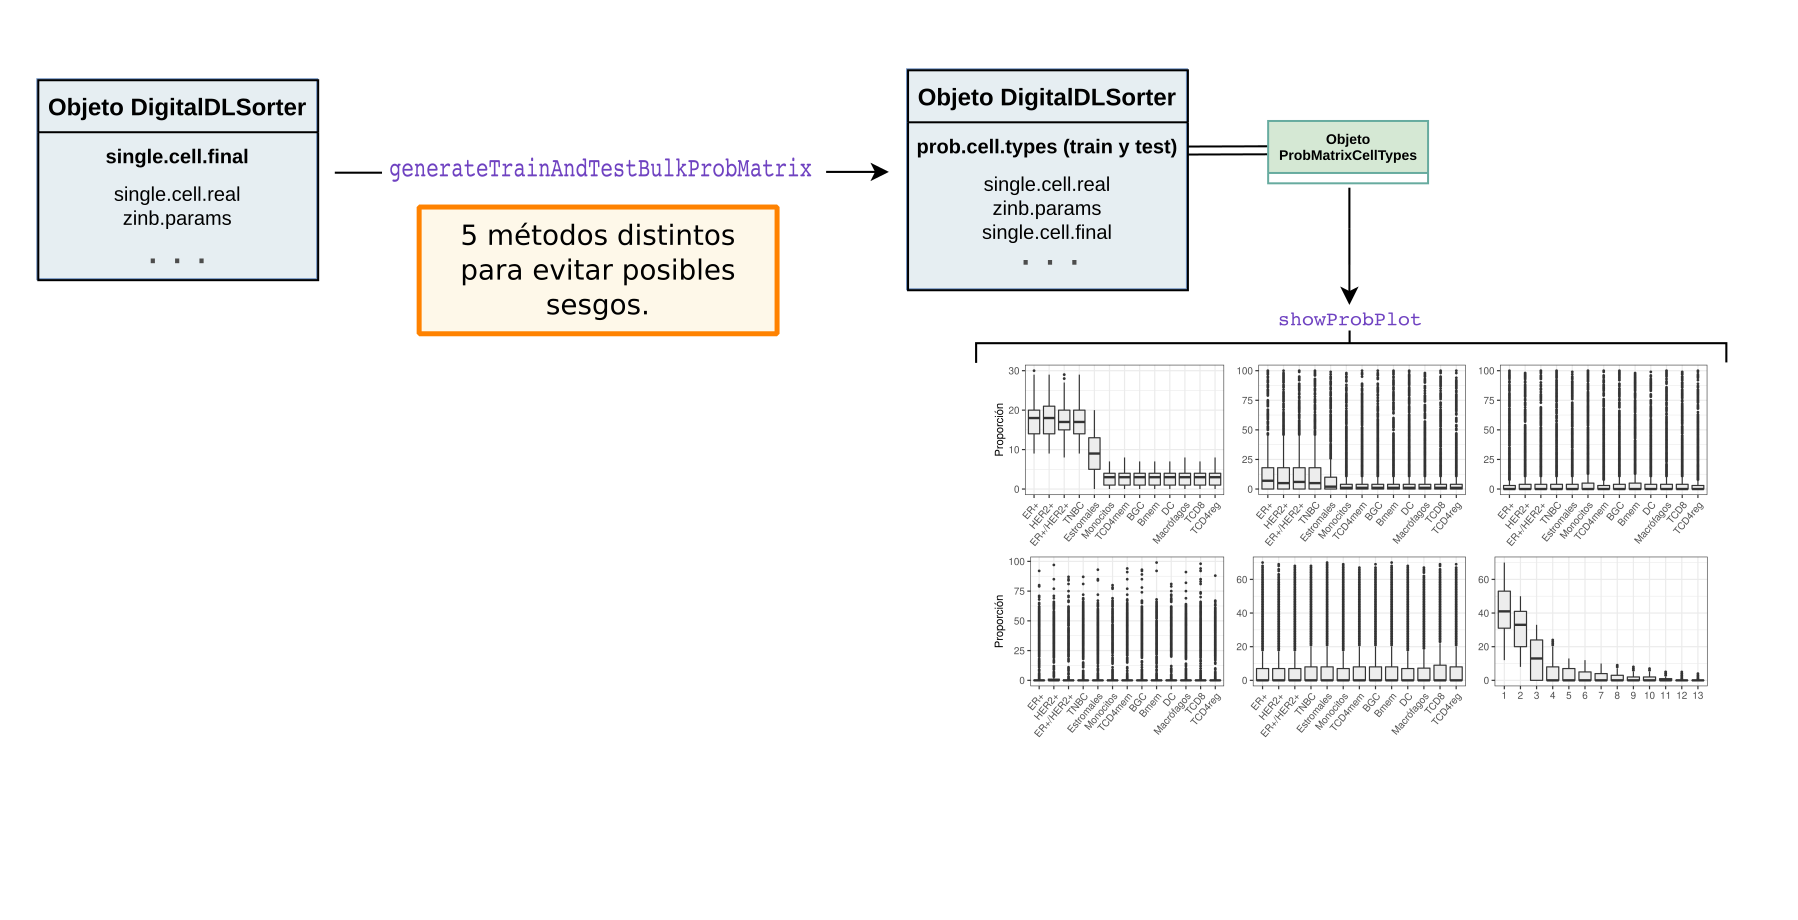
\includegraphics[width=12cm]{images/generateBulkMatrix_1_fixed_1.png}
    \end{figure}
  }

  \only<2>{
    \begin{figure}
      \centering
      \vskip-3em
      % \vskip1mm
      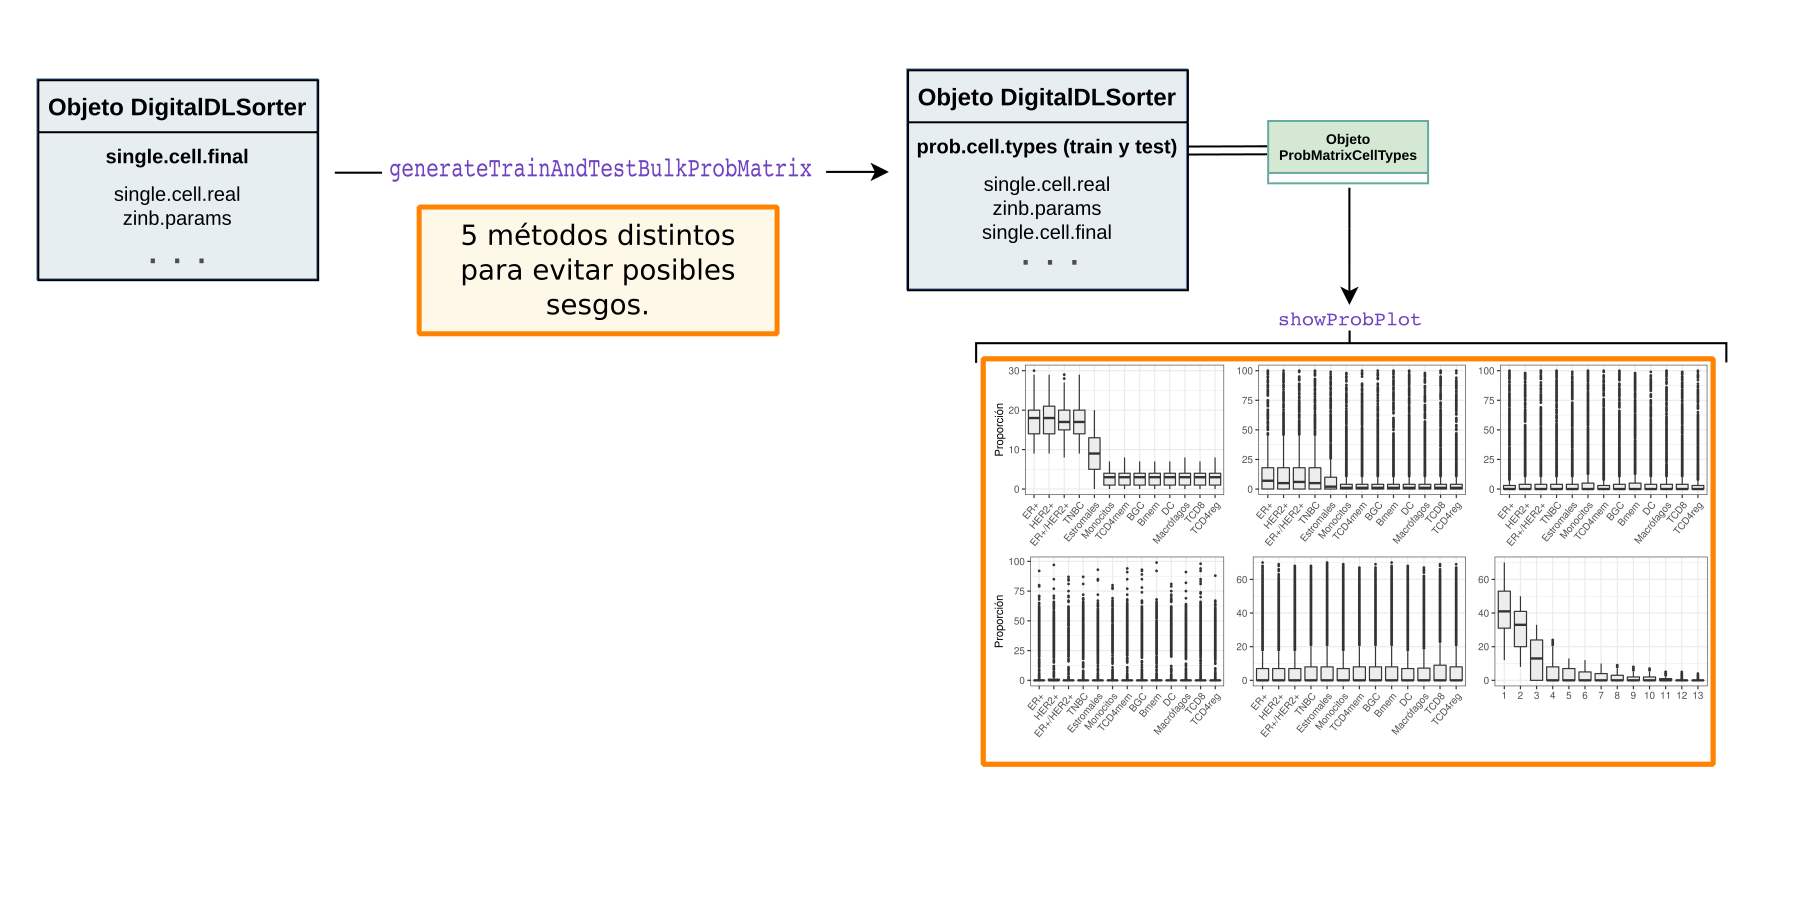
\includegraphics[width=12cm]{images/generateBulkMatrix_2_fixed_1.png}
    \end{figure}
  }

  \only<3>{
    \begin{figure}
      \centering
      \vskip-2em
      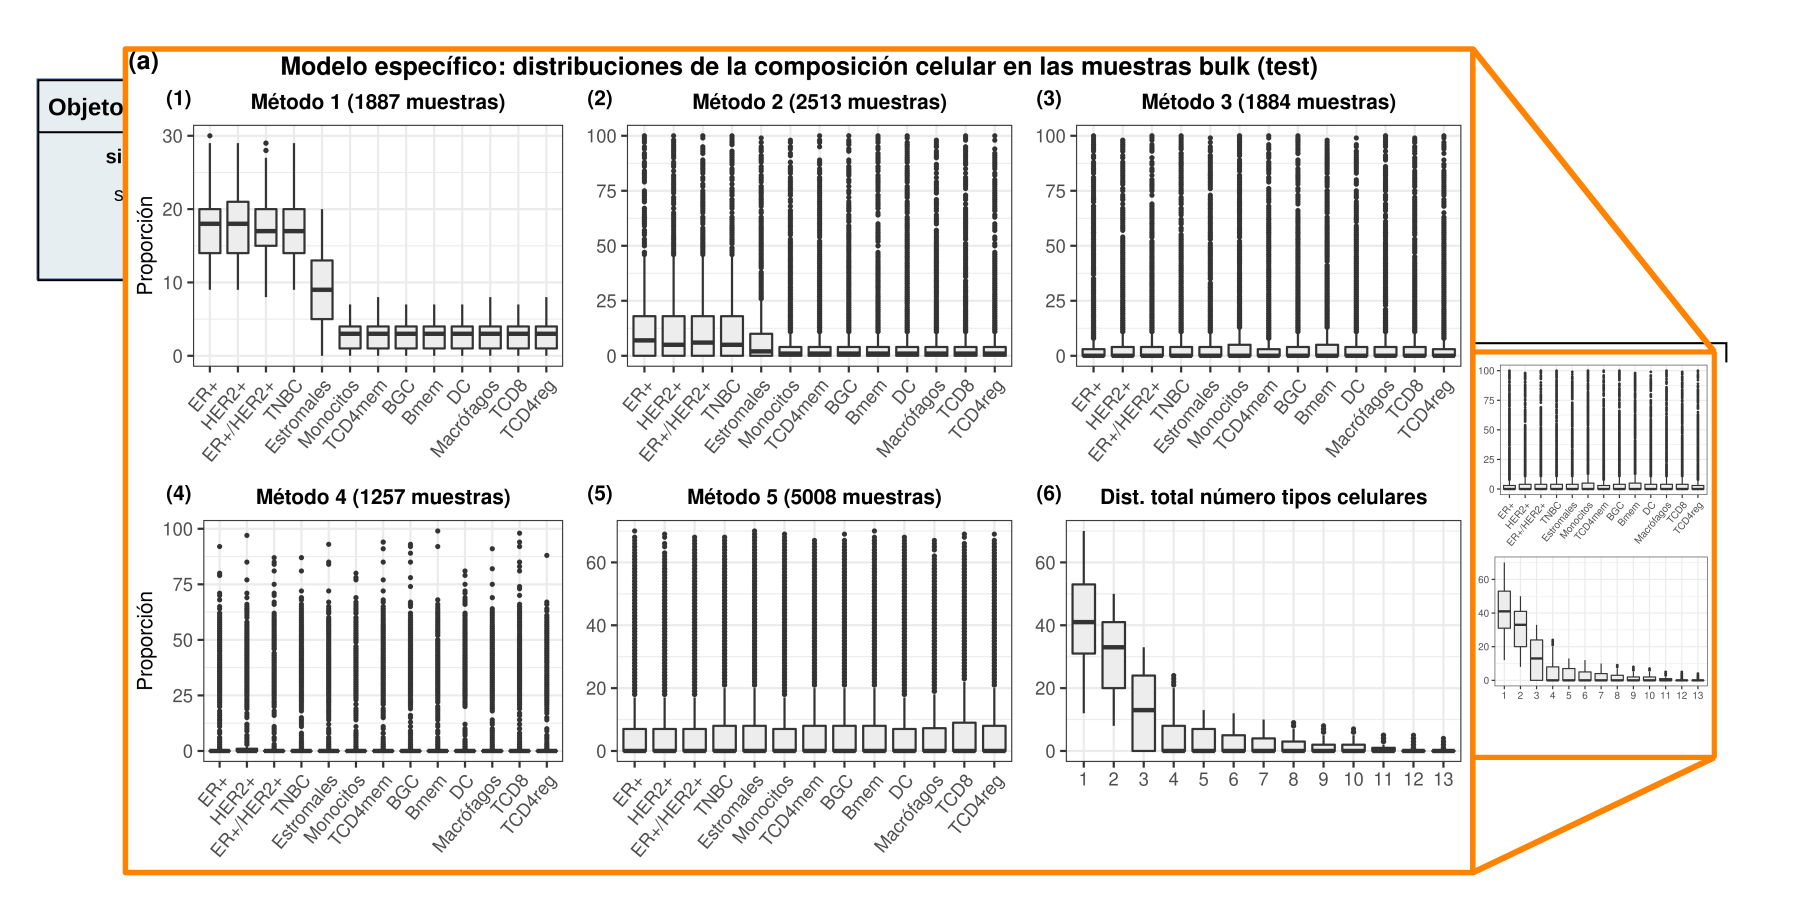
\includegraphics[width=11cm]{images/generateBulkMatrix_3_1.png}
    \end{figure}
  }

  \begin{textblock*}{\textwidth}(0.5cm,7cm)
    \Fontvi
    \begin{itemize}
      \item Generación de un objeto \textit{ProbMatrixCellTypes} en el slot \textit{prob.cell.types}.
      \item 6 métodos distintos para evitar posibles sesgos en la composición de las muestras \textit{bulk}.
      \item Perfiles \textit{single-cell} son separados en entrenamiento y test.
    \end{itemize}
  \end{textblock*}
\end{frame}


\begin{frame}[fragile,t]{2. Generación de la matriz de composición celular}
  \lstinputlisting[]{./boxcodes/boxcode4.R}
\end{frame}

% Simulación de perfiles bulk y preparación de los datos para el entrenamiento -----

\begin{frame}[fragile]{3. Simulación de perfiles \textit{bulk} y preparación de los datos}

  \begin{figure}
    \centering
    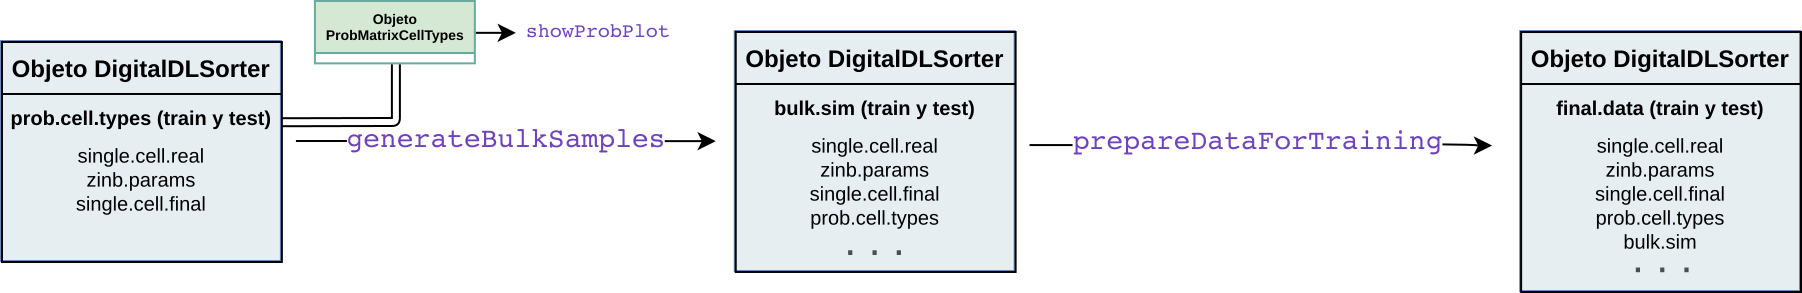
\includegraphics[width=13cm]{images/bulkSimulation_1.png}
  \end{figure}

  % \begin{textblock*}{\textwidth}(0.5cm,7.3cm)
  \begin{enumerate}
    \item Simulación de los perfiles \textit{bulk} de acuerdo a las proporciones y al número de células establecidas en el paso anterior.
    \item Preparación de los datos para el entrenamiento de la red neuronal y su evaluación: combinación de perfiles, normalización...
  \end{enumerate}
  % \end{textblock*}  
\end{frame}


\begin{frame}[fragile]{3. Simulación de perfiles \textit{bulk}}

  % \vskip-0.5em
  \begin{figure}
    \centering
    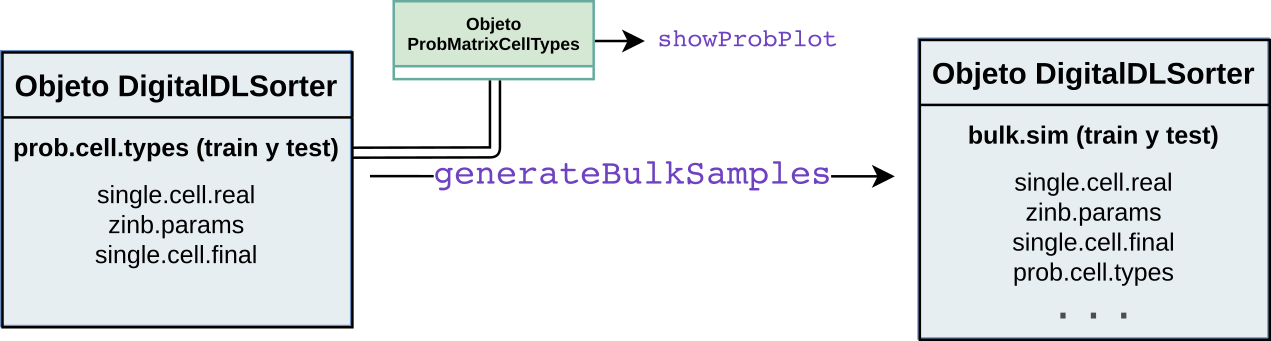
\includegraphics[width=10cm]{images/simulBulk_1_1.png}
  \end{figure}

  \begin{columns}
    \begin{column}{0.4\textwidth}
      \begin{equation*}
        T_{ij} = \sum_{k = 1}^{K} \sum_{z = 1}^Z C_{izk}
      \end{equation*}

      \begin{equation*}
        \arraycolsep=1pt\def\arraystretch{1}
        \textrm{de forma que} \left\{
        \begin{array}{l}
          i = 1 \ldots M                \\
          j = 1 \ldots N                \\
          Z = 1 \ldots 100 \cdot P_{jk} \\
          \sum_{k = 1}^K Z \cdot P_{jk} = 100
        \end{array}
        \right.
      \end{equation*}
    \end{column}

    \begin{column}{0.65\textwidth}
      \Fontvi
      \begin{itemize}
        \item Sumatorio de \texttt{n.cells} (100 en este caso) perfiles \textit{single-cell} ($z$) en función del tipo celular ($k$) al que pertenezcan para cada muestra \textit{bulk} ($j$).
        \item Implementación: posibilidad de utilizar ficheros HDF5 como \textit{back-end}: paquetes DelayedArray y HDF5Array.
      \end{itemize}
      \begin{beamercolorbox}[sep=0.2cm,center]{coloredboxstuff}
        2 matrices de 23.555 filas y 18.777 columnas:\\6,5GB $\rightarrow$ 4,4kB
      \end{beamercolorbox}
    \end{column}
  \end{columns}
\end{frame}

\begin{frame}[fragile]{3. Preparación de los datos para entrenamiento y evaluación}

  \vskip-0.5em
  \begin{figure}
    \centering
    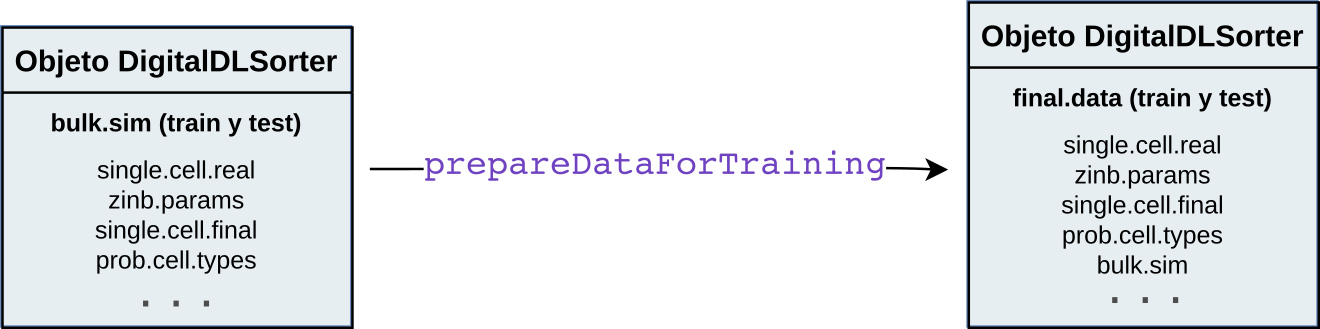
\includegraphics[width=10cm]{images/preparingSamples_1.png}
  \end{figure}

  \begin{itemize}
    \item Combinación de perfiles mediante el argumento \texttt{combine}:
          \begin{itemize}
            \item Solo perfiles \textit{single-cell}.
            \item Solo perfiles \textit{bulk}.
            \item Combinación de ambos.
          \end{itemize}
    \item Normalización: cálculo CPM y establecimiento de $\mu = 0$ y $\sigma = 1$
    \item Transposición de la matriz resultante.
  \end{itemize}

  \vskip1em

  \begin{beamercolorbox}[sep=0.2cm,center]{coloredboxstuff}
    Posibilidad de usar ficheros HDF5 $\rightarrow$ rápida lectura de las muestras durante entrenamiento y predicción
  \end{beamercolorbox}

\end{frame}


\begin{frame}[fragile,t]{3. Simulación de perfiles \textit{bulk} y preparación de datos}
  \lstinputlisting[]{./boxcodes/boxcode5.R}
\end{frame}


% Entrenamiento de la red neuronal -------------------------------------------------

\begin{frame}[fragile]{4. Entrenamiento y evaluación del modelo}

  \begin{figure}
    \centering
    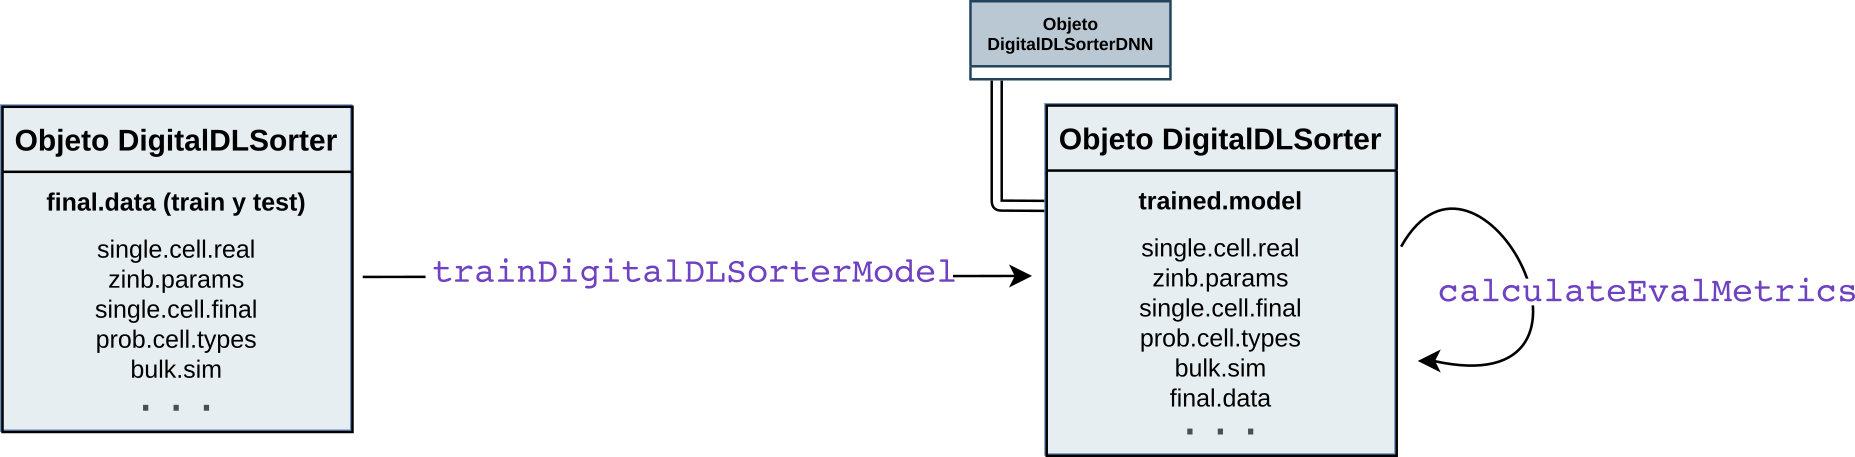
\includegraphics[width=13cm]{images/training_DNN_1.png}
  \end{figure}

  % \begin{textblock*}{\textwidth}(0.5cm,7.3cm)
  \begin{enumerate}
    \item Entrenamiento de la Red Neuronal Profunda con los datos seleccionados en el slot \textit{final.data}.
    \item Cálculo de métricas de error para determinar el desempeño del modelo durante la resolución del problema de deconvolución sobre las muestras de test.
  \end{enumerate}
  % \end{textblock*}  
\end{frame}

\begin{frame}[fragile]{4. Entrenamiento de la Red Neuronal Profunda}
  Uso de los paquetes \alert{Keras} y \alert{Tensorflow}: API de R para el módulo Keras de Python.

  \begin{columns}
    \begin{column}{0.6\textwidth}
      \vskip-1em
      \lstinputlisting[]{./boxcodes/boxcode6.R}
      \Fontvi{
        \begin{alertblock}{Parámetros}
          \begin{itemize}
            \item Número de épocas con \texttt{num.epochs}.
            \item Tamaño de \textit{batch} con \textit{batch.size}.
            \item Subset de validación con \texttt{val} y \texttt{freq.val}.
            \item Función de pérdida con \texttt{loss} (Divergencia de Kullback-Leibler por defecto).
          \end{itemize}
        \end{alertblock}
      }
    \end{column}

    \begin{column}{0.4\textwidth}
      \begin{figure}
        \centering
        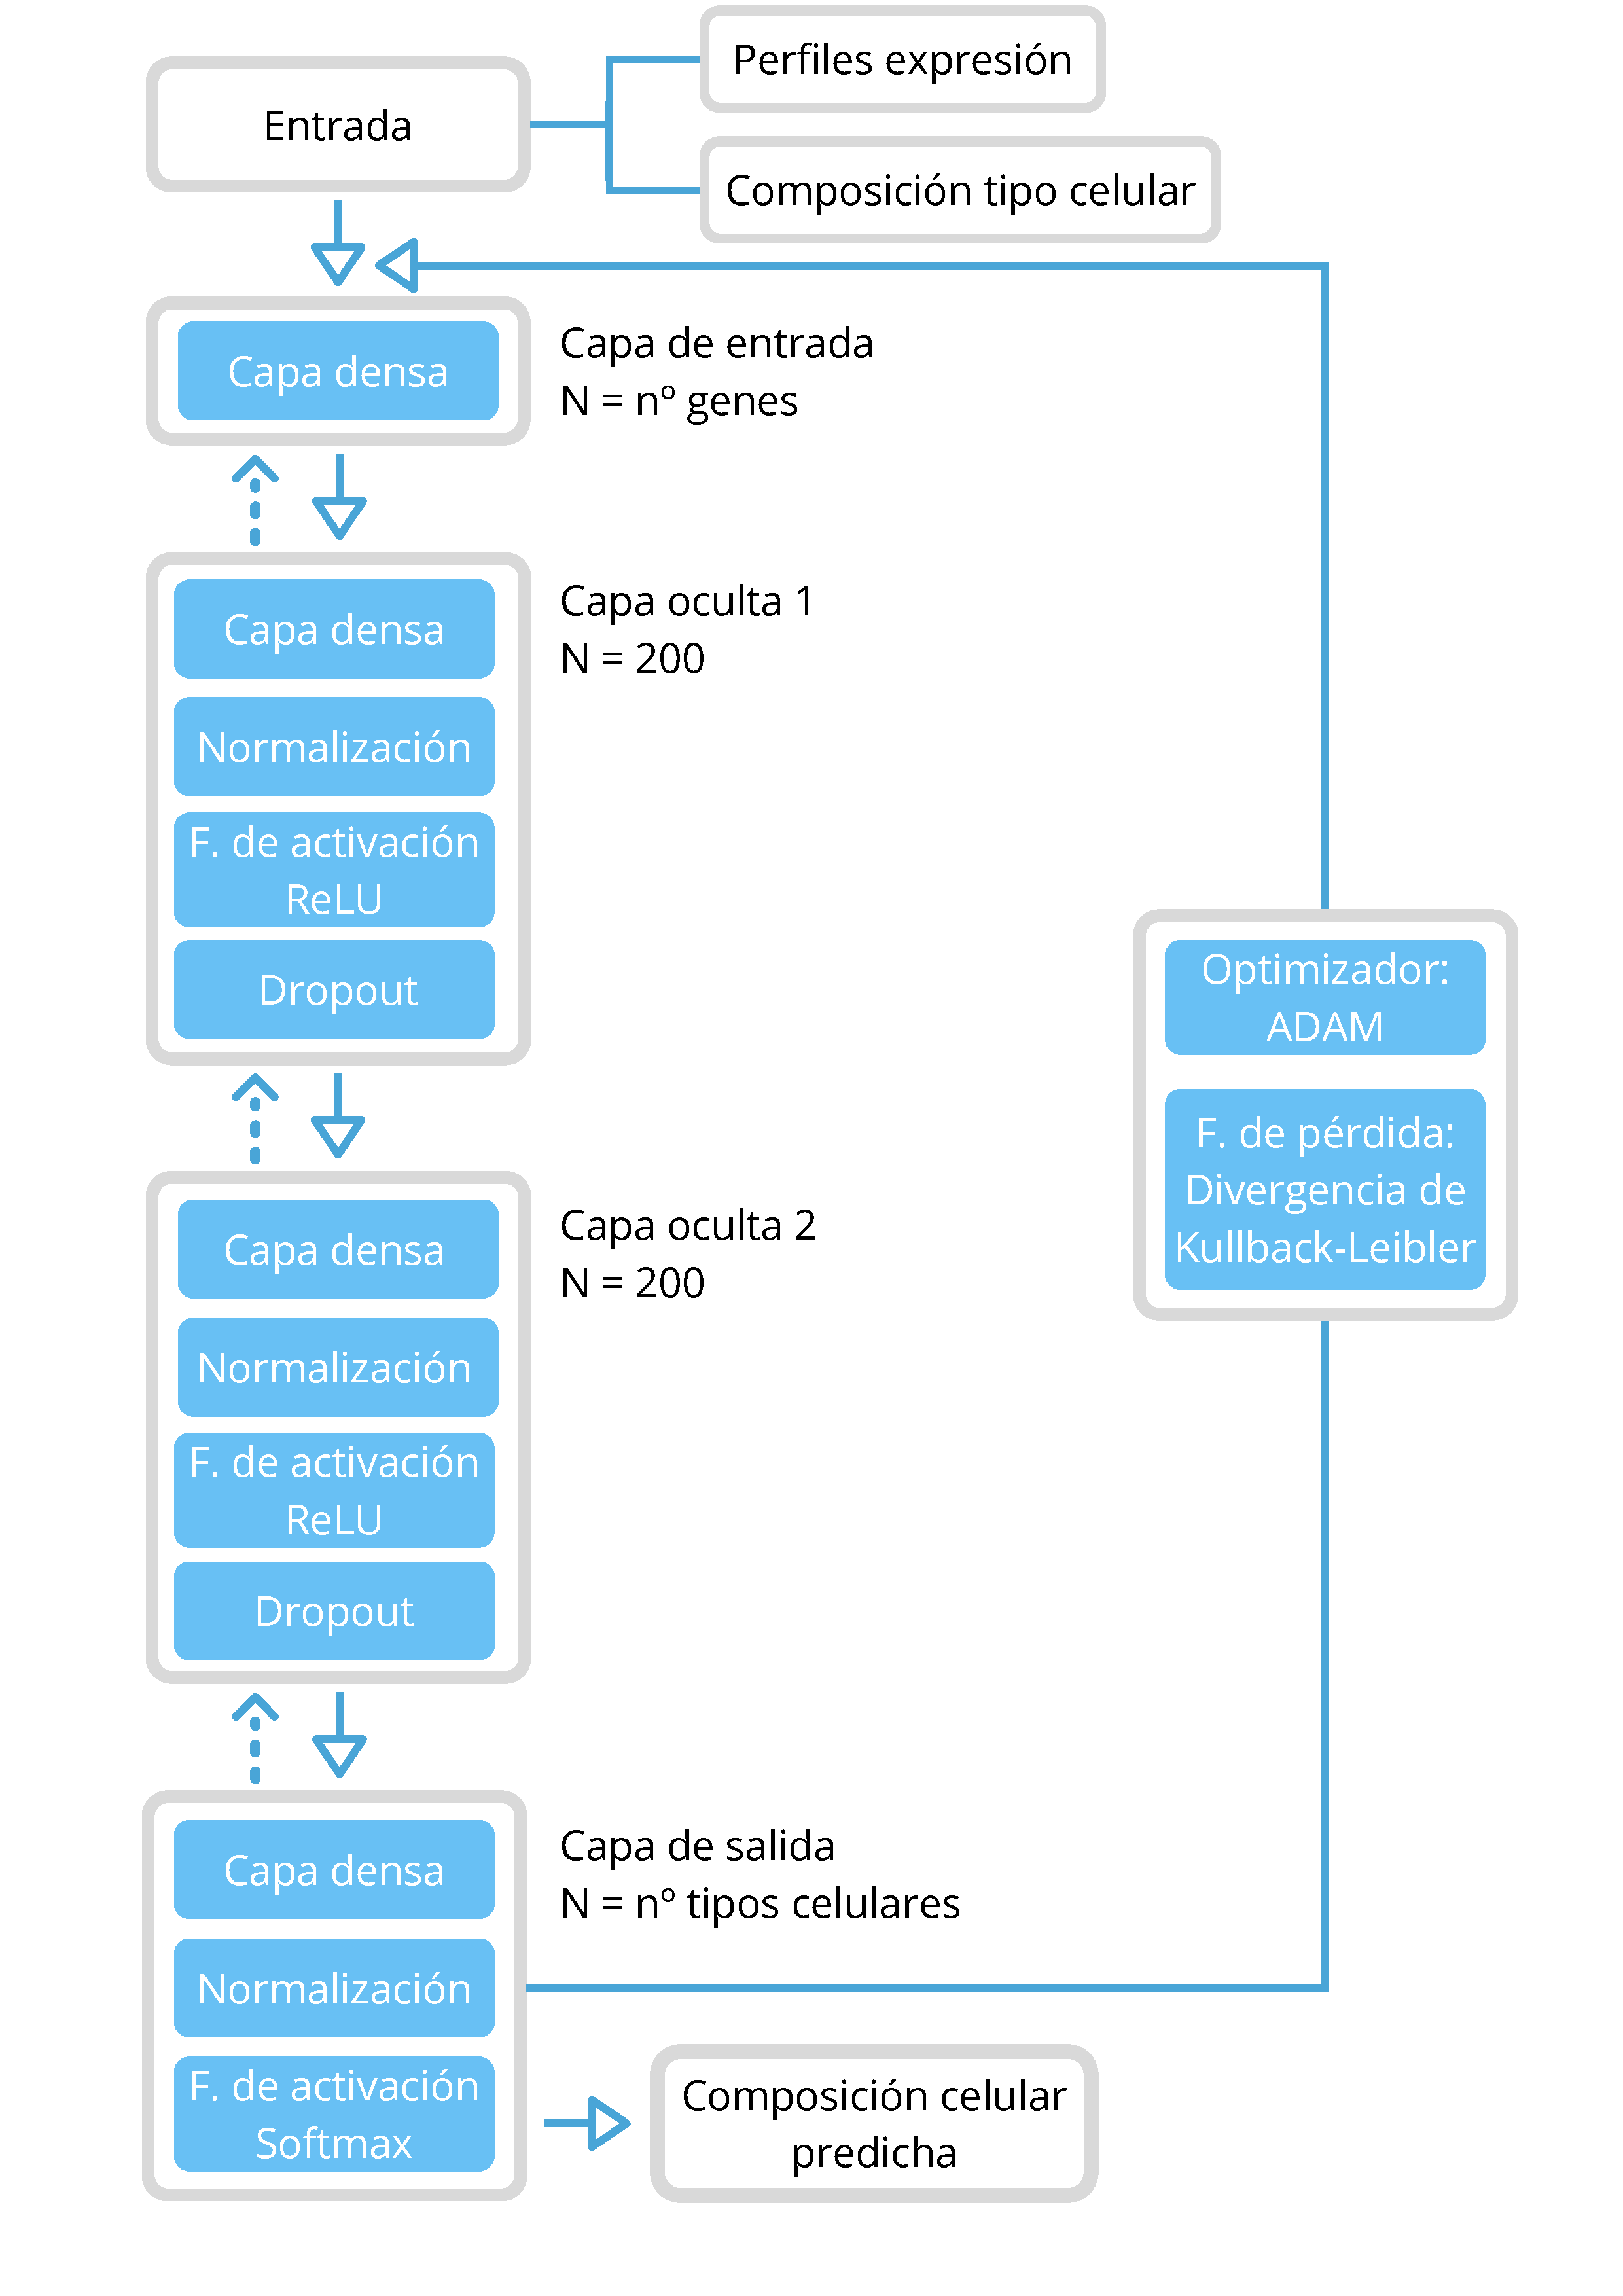
\includegraphics[width=5cm]{images/DiagramNeuralNetwork.pdf}
      \end{figure}
    \end{column}
  \end{columns}
\end{frame}


\begin{frame}[fragile]{4. Evaluación del modelo sobre los datos de test}
  \begin{columns}
    \begin{column}{0.4\textwidth}
      \begin{figure}
        \centering
        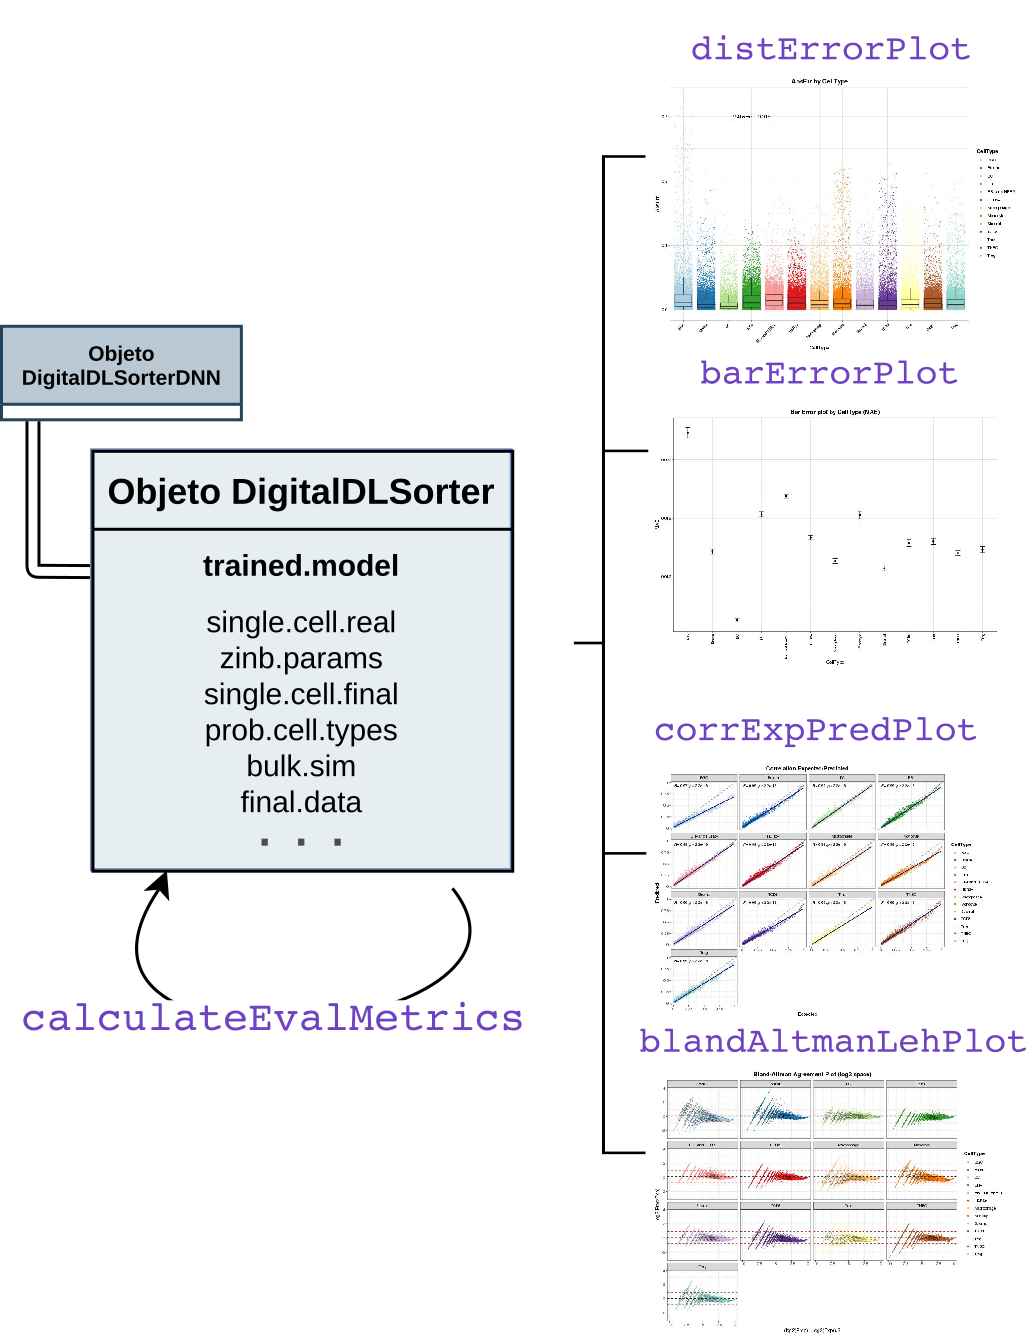
\includegraphics[width=5cm]{images/training_DNN_4_1_1.png}
      \end{figure}
    \end{column}

    \begin{column}{0.6\textwidth}
      \begin{itemize}
        \item \texttt{calculateEvalMetrics}: cálculo de error absoluto y error cuadrático.
        \item \texttt{distErrorPlot} y \texttt{barErrorPlot}: distribución de los errores en función de tipo celular, número de tipos celulares.
        \item \texttt{corrExpPredPlot}: gráficos de correlación $\rightarrow$ coeficiente de correlación de Pearson ($R$) y Coeficiente de correlación de concordancia (CCC).
        \item \texttt{blandAltmanLehPlot}: gráfico de concordancia entre predicción y real.
      \end{itemize}
    \end{column}
  \end{columns}

  \begin{beamercolorbox}[sep=0.2cm,center]{coloredboxstuff}
    Determinación del desempeño del modelo
  \end{beamercolorbox}
\end{frame}

% Meter un link que te lleve a una app shiny en la que generar diferentes plots con las funciones.

\begin{frame}[fragile]{5. Carga de nuevos datos \textit{bulk} y deconvolución}

  \begin{figure}
    \centering
    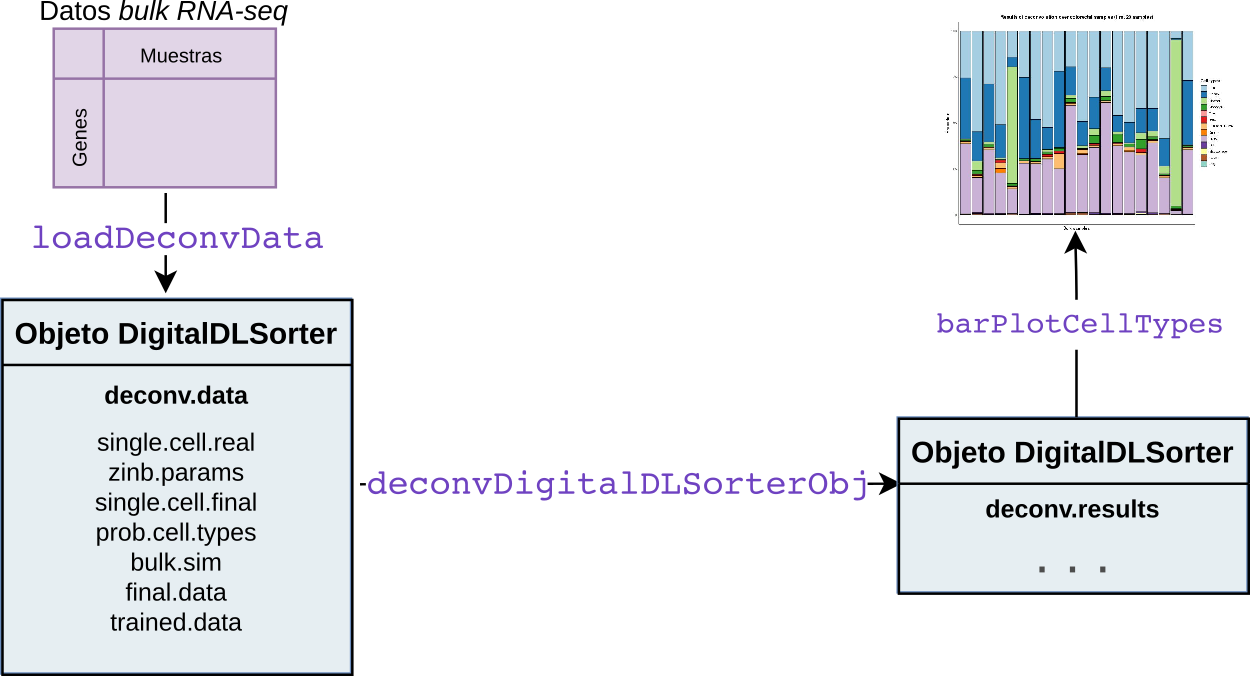
\includegraphics[width=8cm]{images/deconvNewSamples_1.png}
  \end{figure}

  % \begin{textblock*}{\textwidth}(0.5cm,7.3cm)
  \begin{itemize}
    \item Carga de nuevas muestras \textit{bulk} en el objeto \textit{DigitalDLSorter} mediante \texttt{loadDeconvDataFromSummarizedExperiment} o \texttt{loadDeconvDataFromFile}.
    \item Deconvolución y representación.
  \end{itemize}
  % \end{textblock*}  
\end{frame}


\begin{frame}[fragile,t]{5. Carga de nuevos datos \textit{bulk} y deconvolución}
  \lstinputlisting[]{./boxcodes/boxcode8.R}
\end{frame}

% \begin{frame}[fragile,t]{Otras funcionalidades}
%   \begin{itemize}
%     \item Guardar objetos \textit{DigitalDLSorter} como ficheros rds y rda.
%     \item Guardar modelos de Keras como ficheros HDF5.
%   \end{itemize}
% \end{frame}

%%%%%%%%%%%%%%%%%%%%%%%%%%%%%%%%%%%%%%%%%%%%%%%%%%%%%%%%%%%%%%%%%%%%%%%%%%%%%%%%%%%%
%%%%%%%%%%%%%%%%%%%%%%%%%%%%%%%%%%%%% ANÁLISIS %%%%%%%%%%%%%%%%%%%%%%%%%%%%%%%%%%%%%
%%%%%%%%%%%%%%%%%%%%%%%%%%%%%%%%%%%%%%%%%%%%%%%%%%%%%%%%%%%%%%%%%%%%%%%%%%%%%%%%%%%%


\section[Análisis de datos \textit{scRNA-seq}]{Análisis de datos \textit{scRNA-seq}}


\begin{frame}{Datos utilizados}

  Datos \textit{scRNA-seq} de \alert{cáncer de mama} procedentes del artículo Chung at al., 2017.
  \vskip3mm
  \begin{columns}
    \begin{column}{0.4\textwidth}
      \begin{itemize}
        \item Se utilizaron las lecturas obtenidas de la base de datos SRA (\href{https://trace.ncbi.nlm.nih.gov/Traces/sra/?study=SRP066982}{SRP066982}).
        \item 11 pacientes que representan los 4 subtipos de cáncer de mama.
        \item Total células: 549.
      \end{itemize}
    \end{column}
    \begin{column}{0.6\textwidth}
      \Fonteight{
        \begin{table}[!h]
          \centering
          \begin{tabular}{cccc}
            \toprule
            \textbf{Paciente} & \textbf{Subtipo} & \textbf{Tejido}  & \textbf{\# células} \\
            \midrule
            BC01              & Luminal A        & Tumor primario   & 26                  \\
            BC02              & Luminal A        & Tumor primario   & 56                  \\
            BC03              & Luminal B        & Tumor primario   & 37                  \\
            BC04              & HER2             & Tumor primario   & 59                  \\
            BC05              & HER2             & Tumor primario   & 77                  \\
            BC06              & HER2             & Tumor primario   & 25                  \\
            BC07              & TNBC             & Tumor primario   & 51                  \\
            BC08              & TNBC             & Tumor primario   & 23                  \\
            BC09              & TNBC             & Tumor primario   & 60                  \\
            BC10              & TNBC             & Tumor primario   & 16                  \\
            BC11              & TNBC             & Tumor primario   & 11                  \\
            BC03LN            & Luminal B        & Tejido linfático & 55                  \\
            BC07LN            & TNBC             & Tejido linfático & 53                  \\
            \bottomrule
          \end{tabular}
        \end{table}
      }
    \end{column}
  \end{columns}
\end{frame}

\begin{frame}[fragile]{Análisis: separación de células tumorales y no tumorales}

  \vskip0.5em

  \Fontvi{
    \alert{--} Alineamiento y cuantificación con \alert{RSEM} y \alert{STAR}.

    \alert{--} Análisis de datos \textit{scRNA-seq} mediante el paquete de R \alert{Seurat}.
  }
  \tikzstyle{format} = [draw=Orange, line width=0.25mm, thin, fill=OrangeBackground, rounded corners=0.25ex, align=center]
  \tikzstyle{medium} = [ellipse, draw=BlueBorder, thin, fill=BlueBackground, minimum height=2.5em, align=center]
  \begin{center}
    \begin{tikzpicture}[node distance=2cm,>=latex', inner sep = 4pt, auto,>=latex', thick, scale=0.6, every node/.style={scale=0.6}]
      % We need to set at bounding box first. Otherwise the diagram
      % will change position for each frame.
      % \path[use as bounding box] (-1,0) rectangle (10,-2);
      \path[->] node[format] (align) {Alineamiento\\y cuantificación};
      \path[->] node[format, right = of align] (filt) {Filtrado y\\normalización}
      (align) edge node {} (filt);
      \path[->] node[format, right = of filt] (dim) {Reducción de dimensionalidad\\y clusterización}
      (filt) edge node {} (dim)
      node[medium, below of=filt] (cell) {488 células\\761 genes}
      (filt) edge node {} (cell)
      node[medium, below of=dim] (clus) {12 PCs\\15 clústeres}
      (dim) edge node {} (clus);
      %       edge node[swap] {xdvi} (screen);
      % \path[->] node[format, right of=ps] (pdf) {.pdf file}
      %               node[medium, below of=ps] (print) {printer}
      %               (ps) edge node {ps2pdf} (pdf)
      %                    edge node[swap] {gs} (screen)
      %                    edge (print);
      % \path[->] (pdf) edge (screen)
      %                     edge (print);
      % \path[->, draw] (tex) -- +(0,1) -| node[near start] {pdf\TeX} (pdf);
    \end{tikzpicture}
  \end{center}

  \vskip-1em

  \begin{columns}
    \begin{column}{0.5\textwidth}
      \begin{figure}
        \centering
        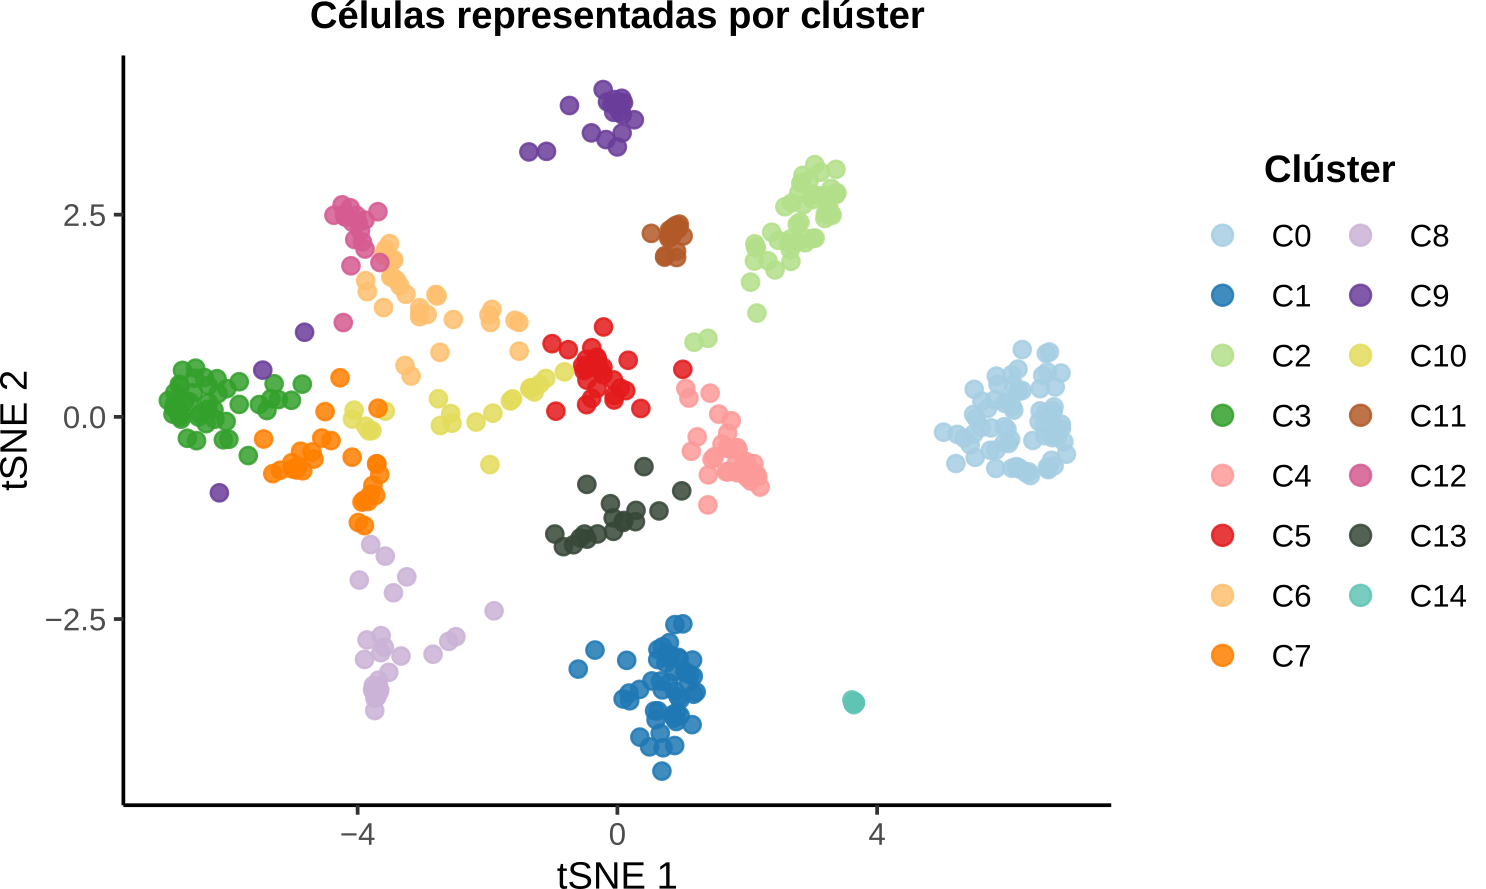
\includegraphics[width=7cm]{images/TSNE_all_def_2.png}
      \end{figure}
    \end{column}
    \begin{column}{0.5\textwidth}
      \begin{itemize}
        \item Filtrado: 488 células.
        \item Normalización: 761 genes más variables.
        \item Reducción de la dimensionalidad: 12 componentes principales.
        \item Clusterización: 15 clústeres.
      \end{itemize}
    \end{column}
  \end{columns}
\end{frame}

\begin{frame}[fragile]{Análisis: separación de células tumorales y no tumorales}

  \begin{columns}
    \begin{column}{0.7\textwidth}
      \Fontvi{Aproximación seguida por los autores del artículo: comparativa de los \alert{patrones de expresión} entre células y tejido mamario normal.}
      \begin{figure}
        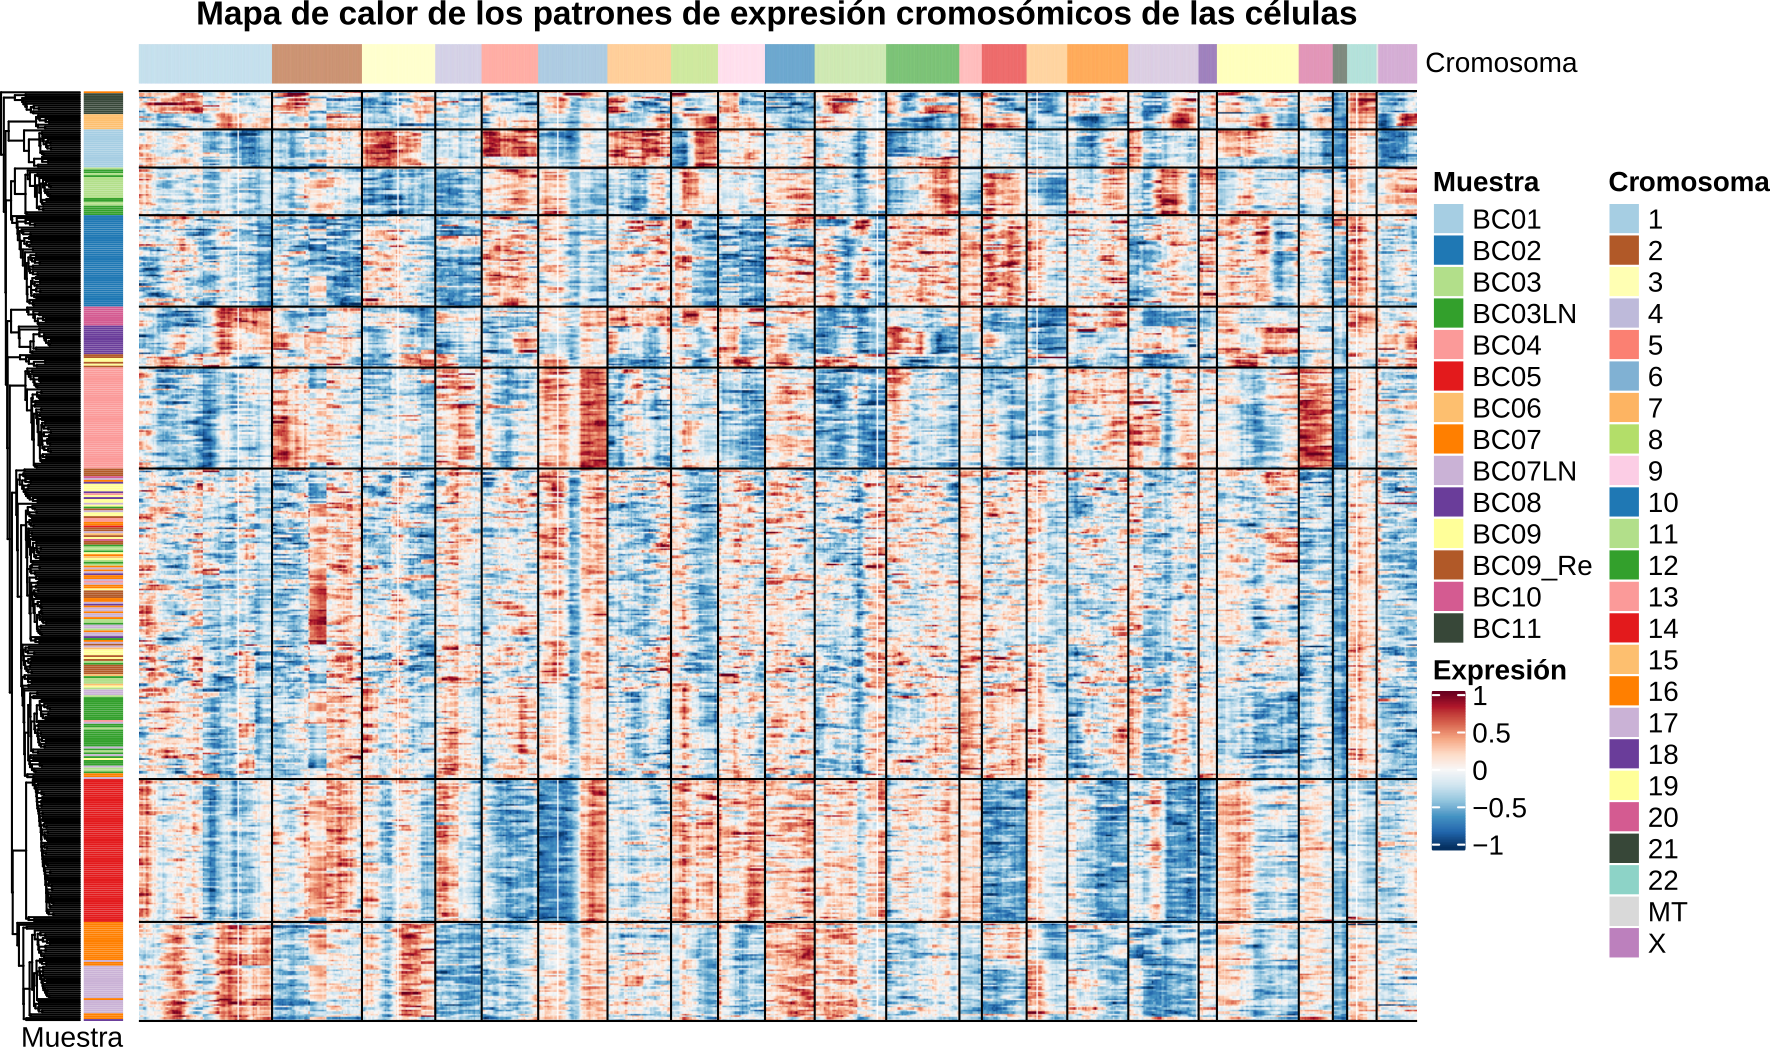
\includegraphics[width=9cm]{images/heatmap_expr_tumor.png}
      \end{figure}
    \end{column}

    \begin{column}{0.4\textwidth}
      \begin{figure}
        \centering
        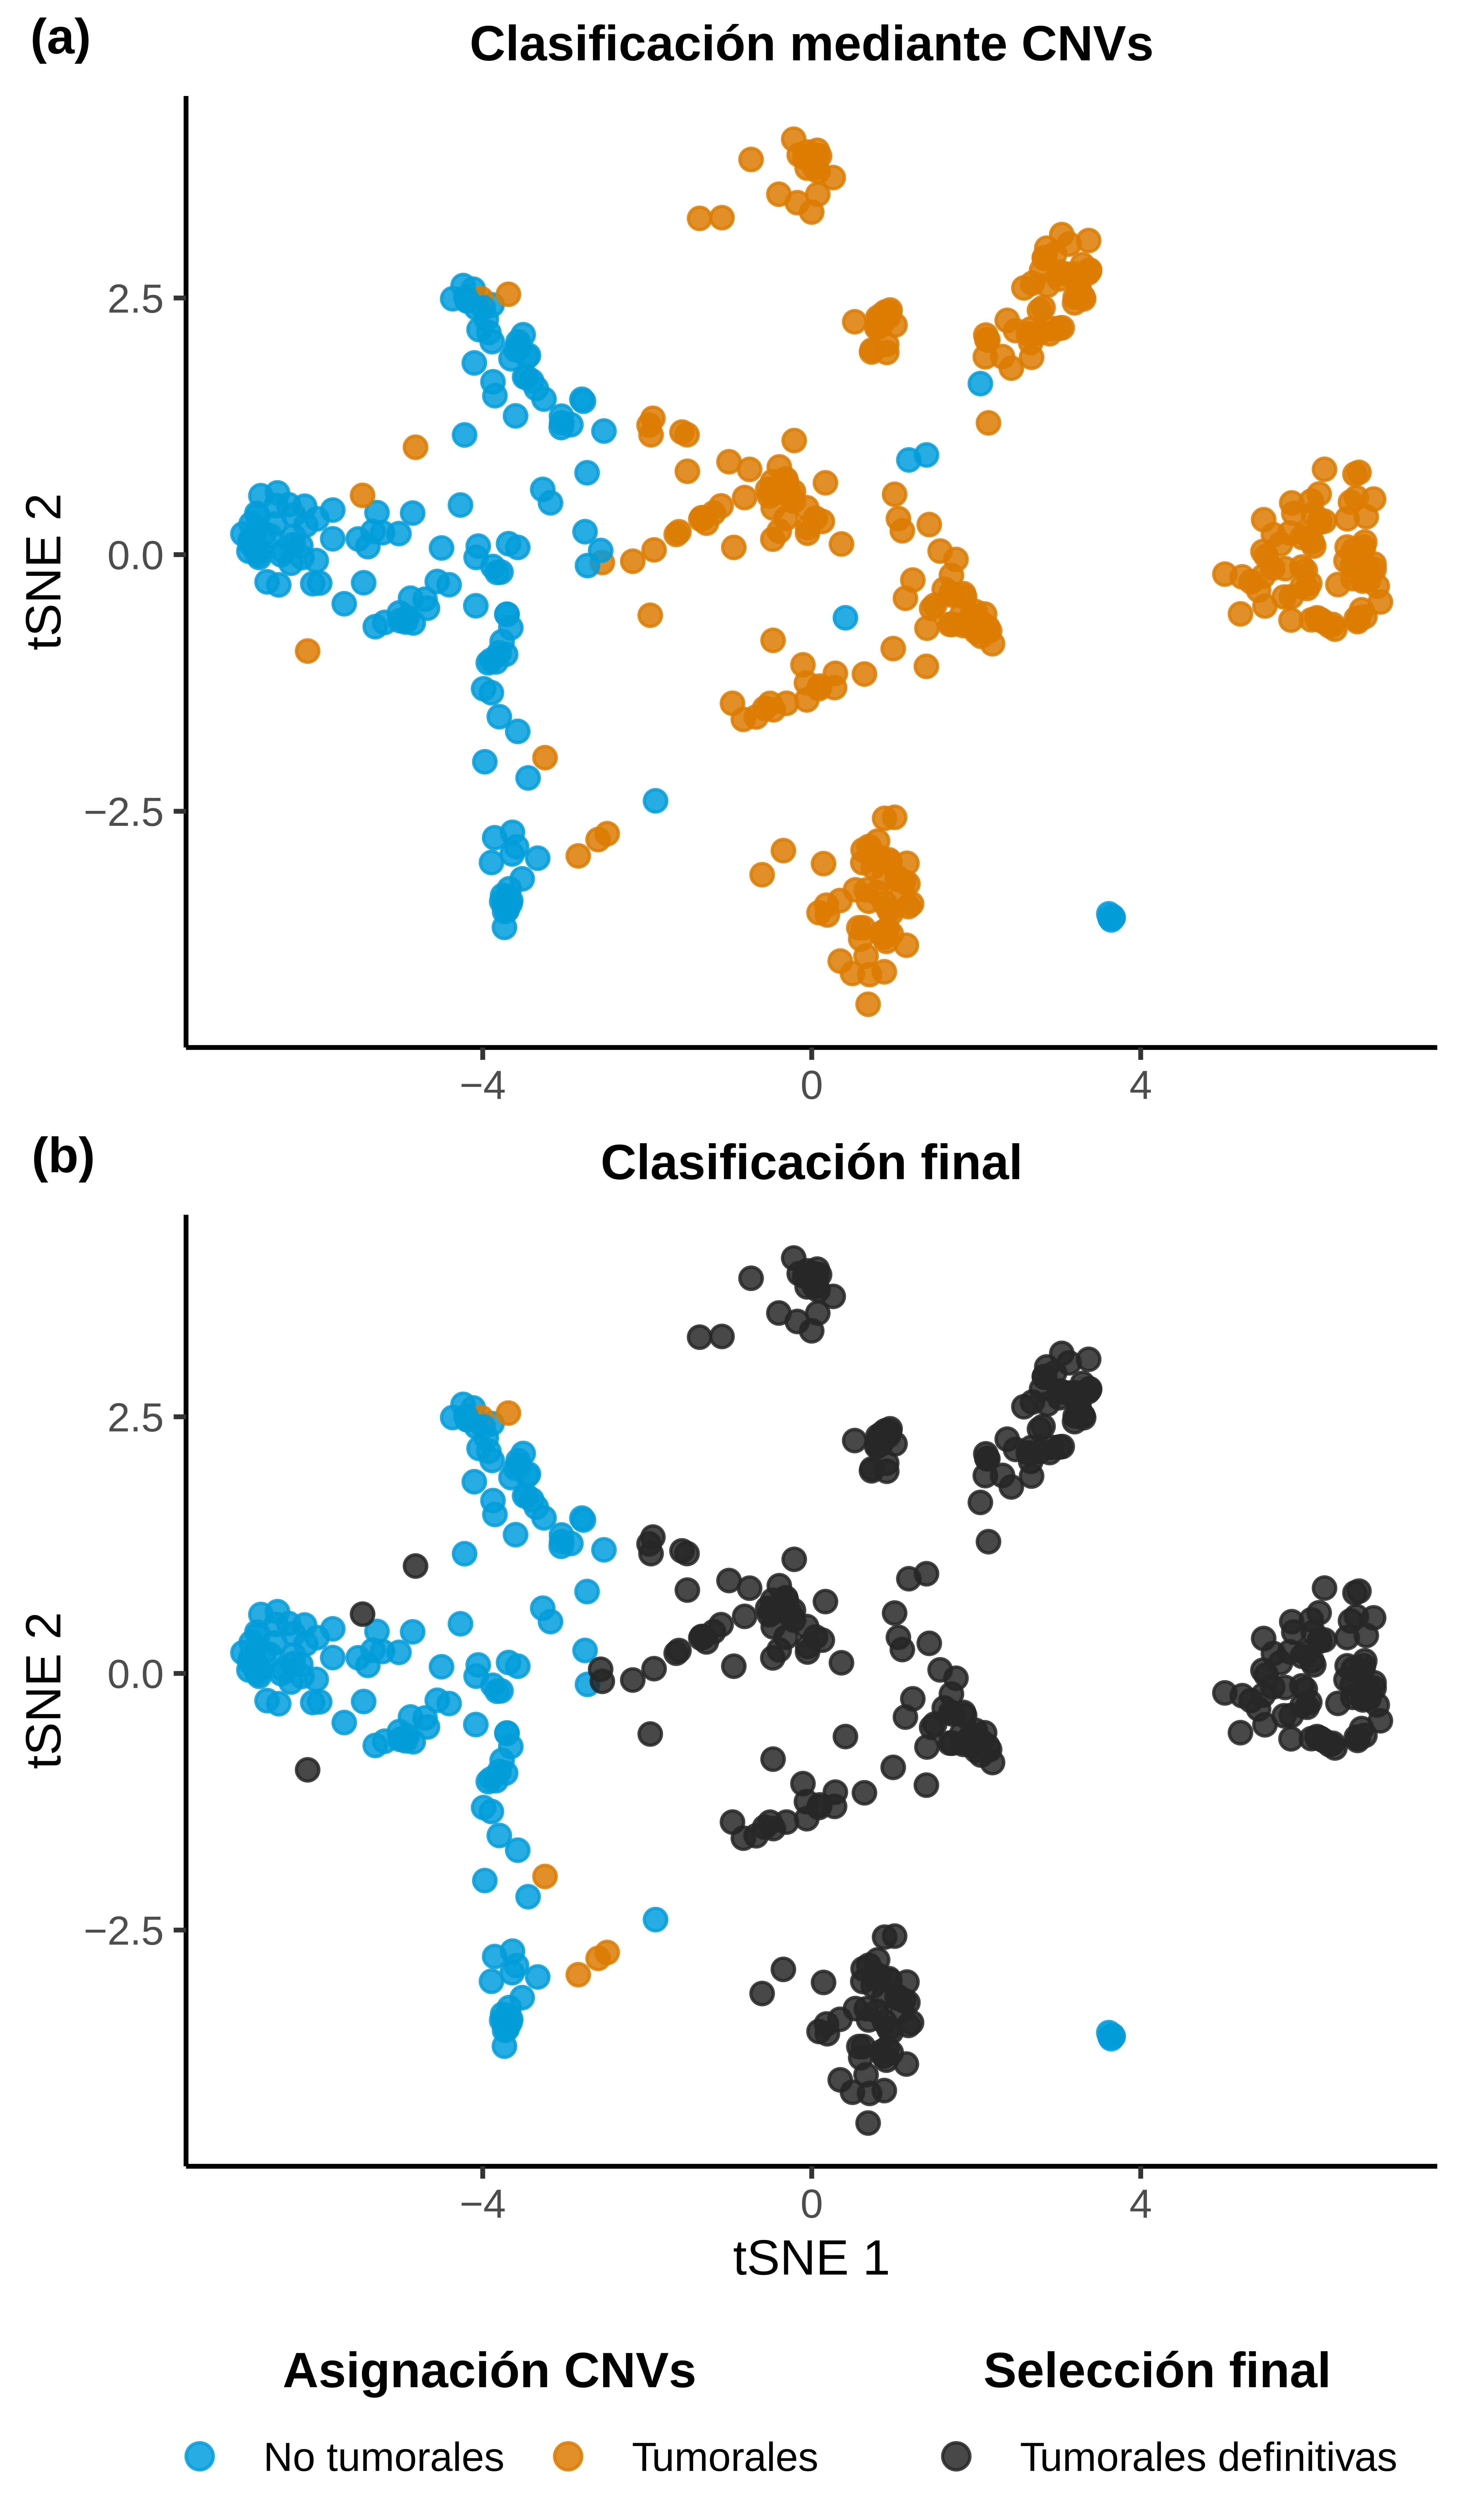
\includegraphics[width=4.2cm]{images/tsne_TumorVnoTumor.png}
      \end{figure}
    \end{column}
  \end{columns}
\end{frame}

\begin{frame}[fragile]{Análisis e identificación de células no tumorales}
  \tikzstyle{format} = [draw=Orange, line width=0.25mm, thin, fill=OrangeBackground, rounded corners=0.25ex, align=center]
  \tikzstyle{medium} = [ellipse, draw=BlueBorder, thin, fill=BlueBackground, minimum height=2.5em, align=center]

  \begin{center}
    \begin{tikzpicture}[node distance=2cm,>=latex', inner sep = 4pt, auto,>=latex', thick, scale=0.6, every node/.style={scale=0.6}]
      \path[->] node[format, right = of align] (filt) {Normalización};
      \path[->] node[format, right = of filt] (dim) {Reducción de dimensionalidad\\y clusterización}
      (filt) edge node {} (dim)
      node[medium, below of=filt] (cell) {733 genes}
      (filt) edge node {} (cell)
      node[medium, below of=dim] (clus) {8 PCs\\10 clústeres}
      (dim) edge node {} (clus);
    \end{tikzpicture}
  \end{center}

  \begin{columns}
    \begin{column}{0.5\textwidth}
      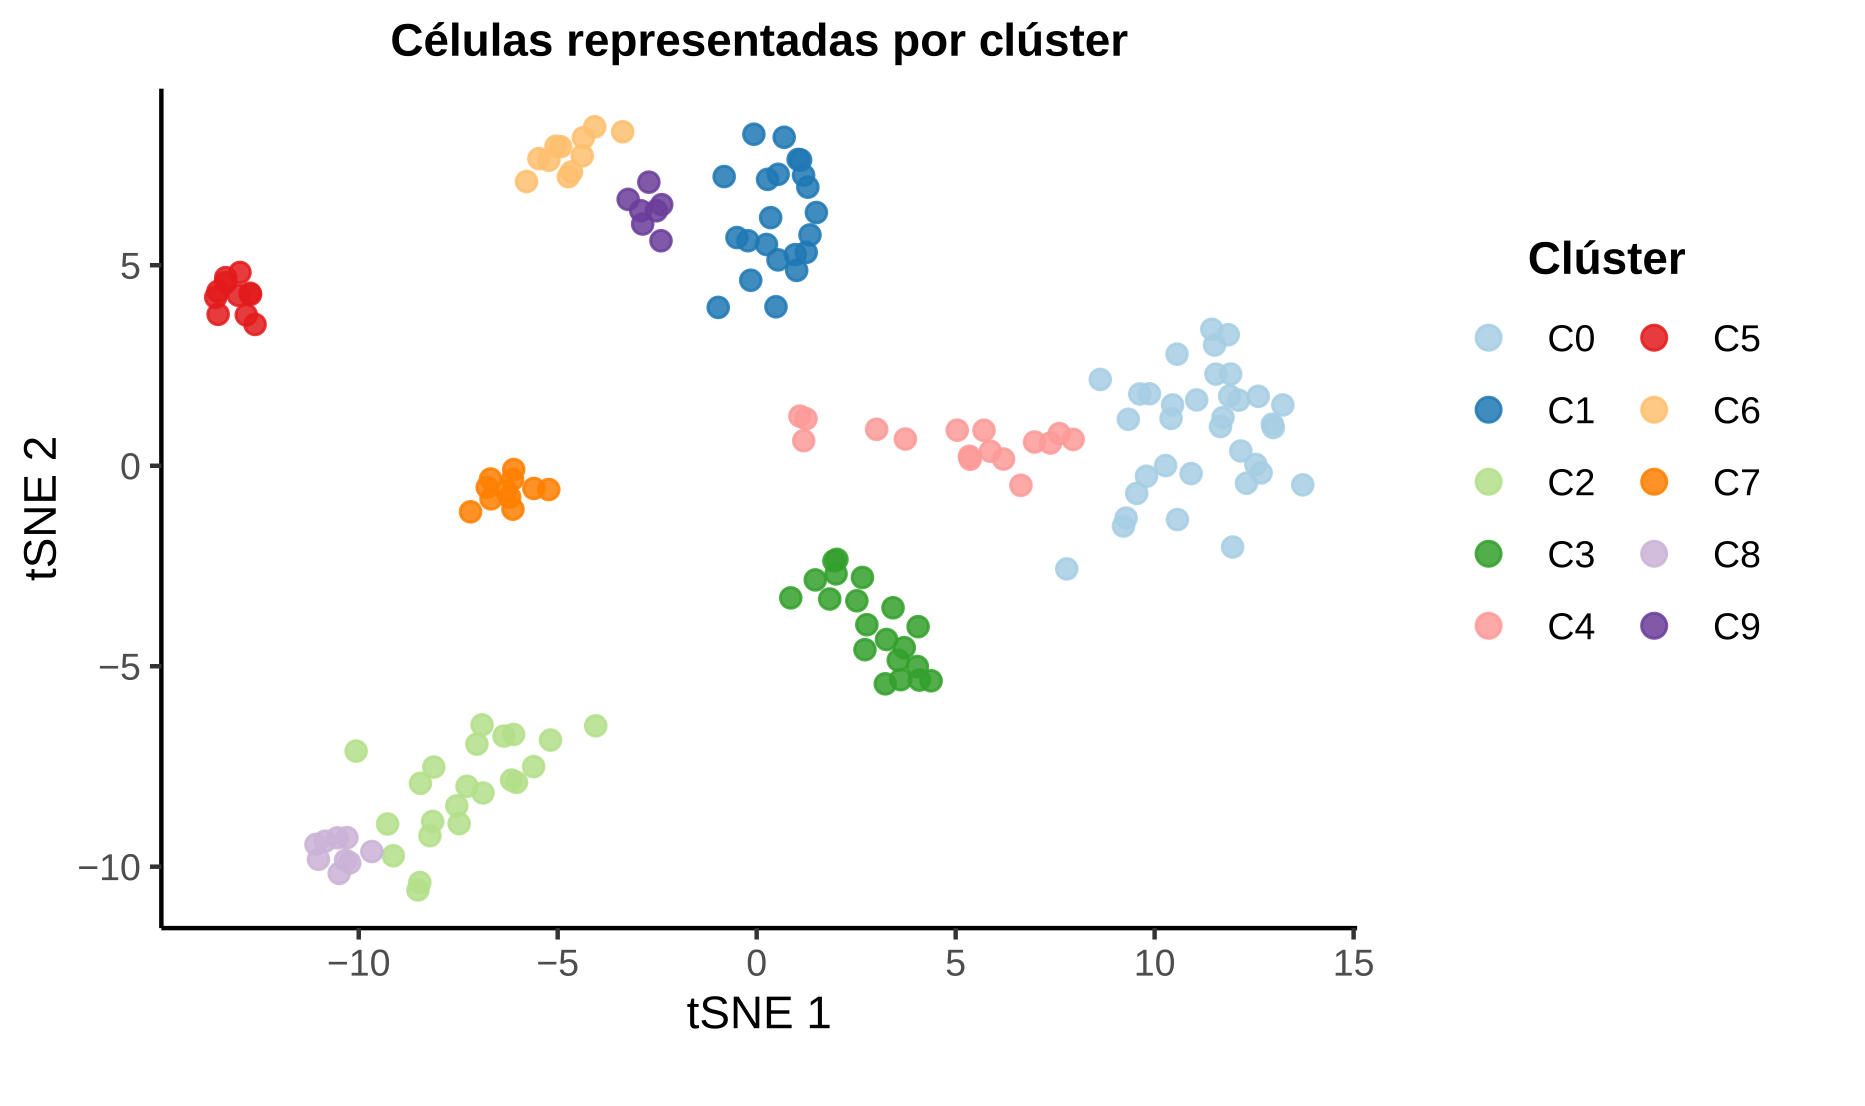
\includegraphics[width=7cm]{images/tsnenoTumorCells_3.png}
    \end{column}
    \begin{column}{0.5\textwidth}
      \begin{itemize}
        \item Normalización: 733 genes más variables.
        \item Reducción de la dimensionalidad: 8 componentes principales.
        \item Clusterización: 9 clústeres.
      \end{itemize}
    \end{column}
  \end{columns}

  % \vskip0.5em
  \begin{beamercolorbox}[sep=0.2cm,center]{coloredboxstuff}
    Caracterización mediante el paquete de R \alert{SingleR}\\y el \alert{análisis manual de marcadores específicos de tipo celular}.
  \end{beamercolorbox}

\end{frame}


\begin{frame}[fragile]{Análisis e identificación de células no tumorales}
  \begin{columns}

    \begin{column}{0.6\textwidth}
      \vskip-1em
      \begin{figure}
        \centering
        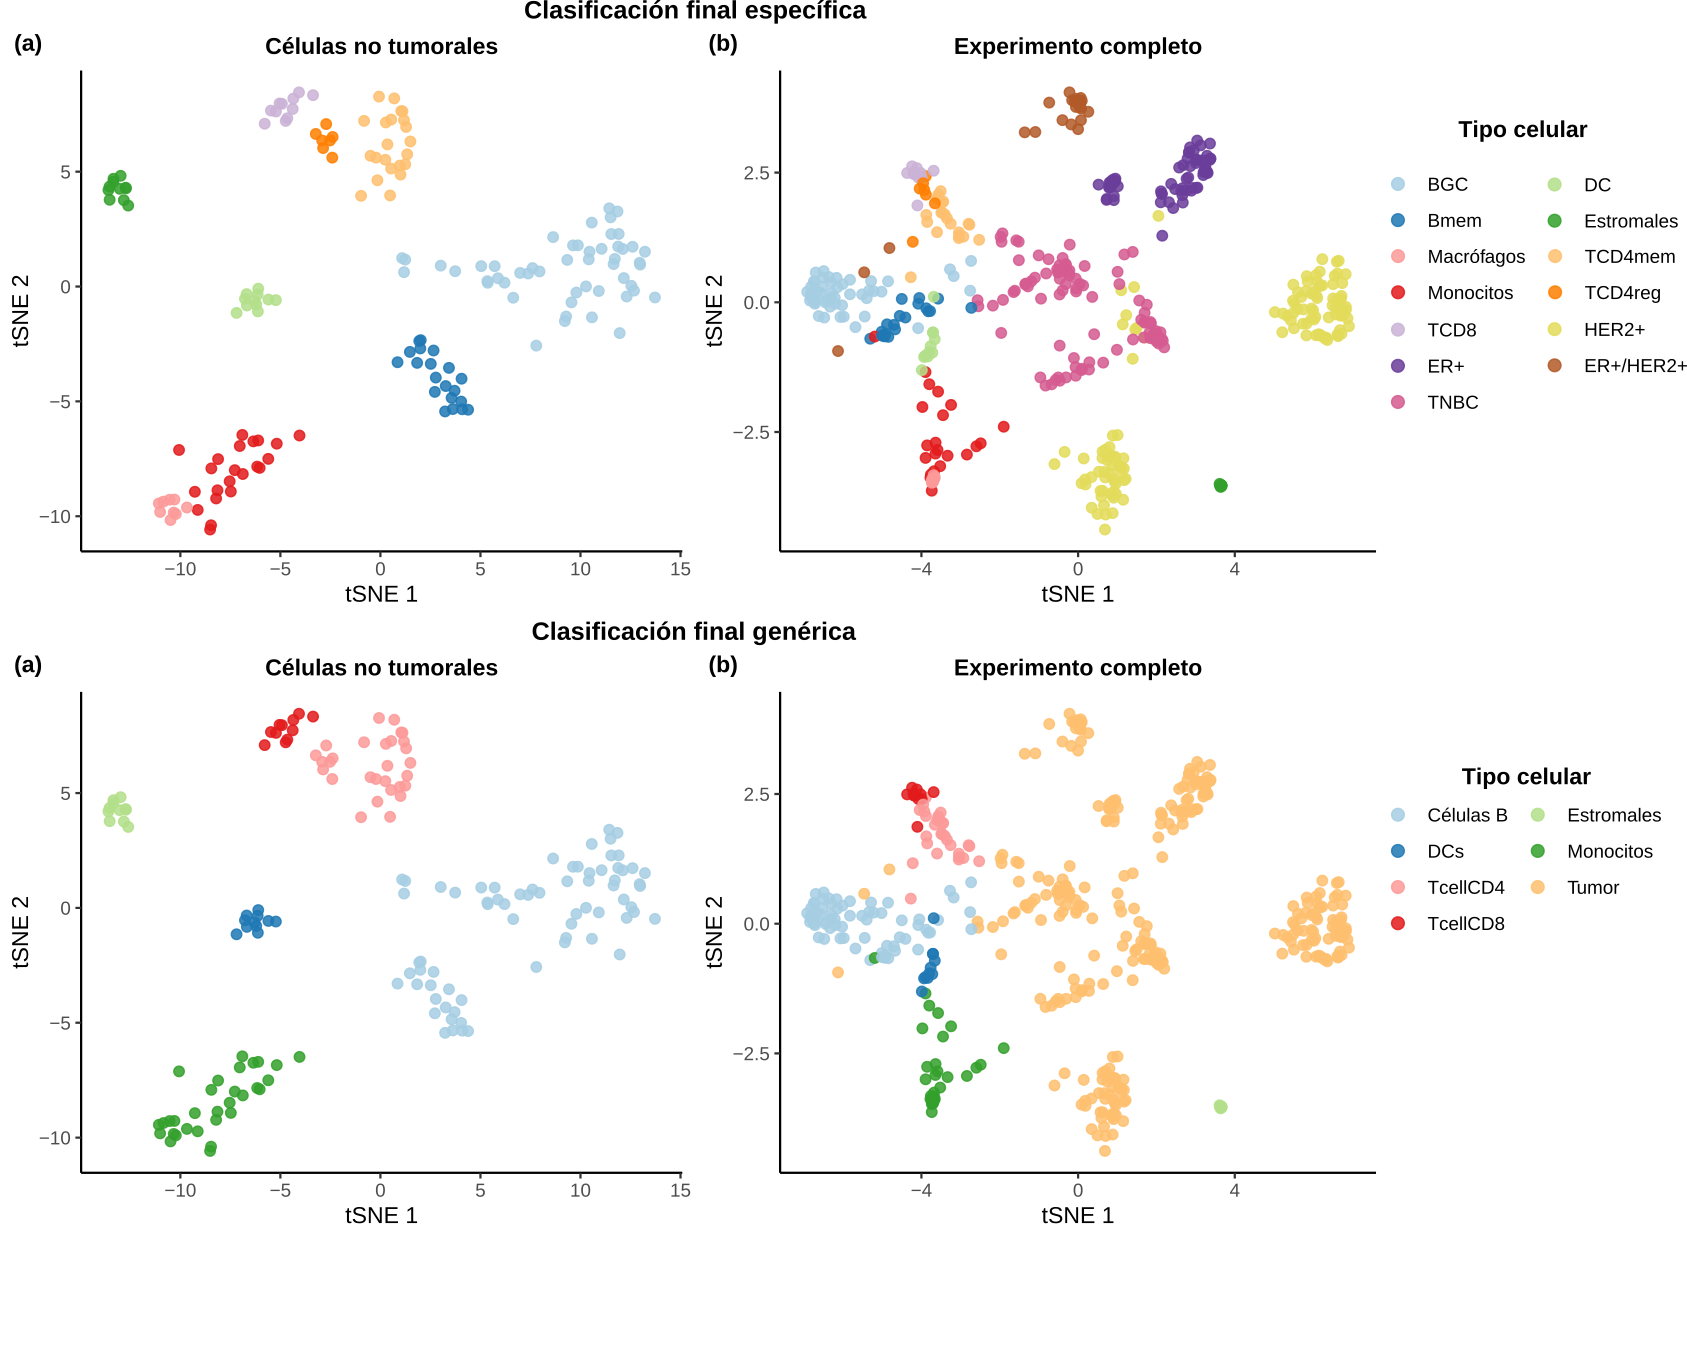
\includegraphics[width=10cm]{images/tsneClassFinal_2.png}
      \end{figure}
    \end{column}

    \begin{column}{0.3\textwidth}
      \begin{textblock*}{3cm}(12cm,2cm)
        \begin{highlightblock}
          \centering
          \Fonteight{Mayor resolución:\\13 tipos celulares}
        \end{highlightblock}
      \end{textblock*}
      \begin{textblock*}{3cm}(12cm,5.5cm)
        \begin{highlightblock}
          \centering
          \Fonteight{Menor resolución:\\7 tipos celulares}
        \end{highlightblock}
      \end{textblock*}
    \end{column}

  \end{columns}

\end{frame}


%%%%%%%%%%%%%%%%%%%%%%%%%%%%%%%%%%%%%%%%%%%%%%%%%%%%%%%%%%%%%%%%%%%%%%%%%%%%%%%%%%%%
%%%%%%%%%%%%%%%%%%%%%%%%%%%%%%%%%%%%%% MODELOS %%%%%%%%%%%%%%%%%%%%%%%%%%%%%%%%%%%%%
%%%%%%%%%%%%%%%%%%%%%%%%%%%%%%%%%%%%%%%%%%%%%%%%%%%%%%%%%%%%%%%%%%%%%%%%%%%%%%%%%%%%

\section[Puesta en práctica de digitalDLSorteR: deconvolución muestras de cáncer de mama]{Puesta en práctica de digitalDLSorteR: deconvolución muestras de cáncer de mama}

\begin{frame}{Modelos}

  Flujo de trabajo mostrado anteriormente:

  \tikzstyle{format} = [draw=Orange, line width=0.25mm, thin, fill=OrangeBackground, rounded corners=0.25ex, align=center]
  \tikzstyle{medium} = [ellipse, draw=BlueBorder, thin, fill=BlueBackground, minimum height=2.5em, align=center]
  \begin{figure}
    \centering
    \begin{tikzpicture}[node distance=0.7cm,>=latex', inner sep = 4pt, auto,>=latex', thick, scale=0.8, every node/.style={scale=0.8}]
      \path[->] node[format] (align) {Estimación parámetros modelo\\ZINB-WaVE y simulación de nuevos\\perfiles \textit{single-cell}};
      \path[->] node[format, right = of align] (filt) {Generación matrices de\\ composición celular\\y simulación perfiles \textit{bulk}}
      (align) edge node {} (filt);
      \path[->] node[format, right = of filt] (dim) {Entrenamiento de la \\Red Neuronal Profunda\\ y evaluación}
      (filt) edge node {} (dim);
    \end{tikzpicture}
  \end{figure}

  Dos modelos de deconvolución a diferente nivel de resolución. Aplicación sobre muestras reales:

  \begin{itemize}
    \item Modelo específico: 13 tipos celulares $\rightarrow$ mayor resolución aunque mayor probabilidad de error.
    \item Modelo genérico: 7 tipos celulares $\rightarrow$ menor resolución aunque menor probabilidad de error.
  \end{itemize}
\end{frame}

\begin{frame}{Estimación parámetros ZINB-WaVE y simulación de nuevas células}
  \begin{figure}
    \centering
    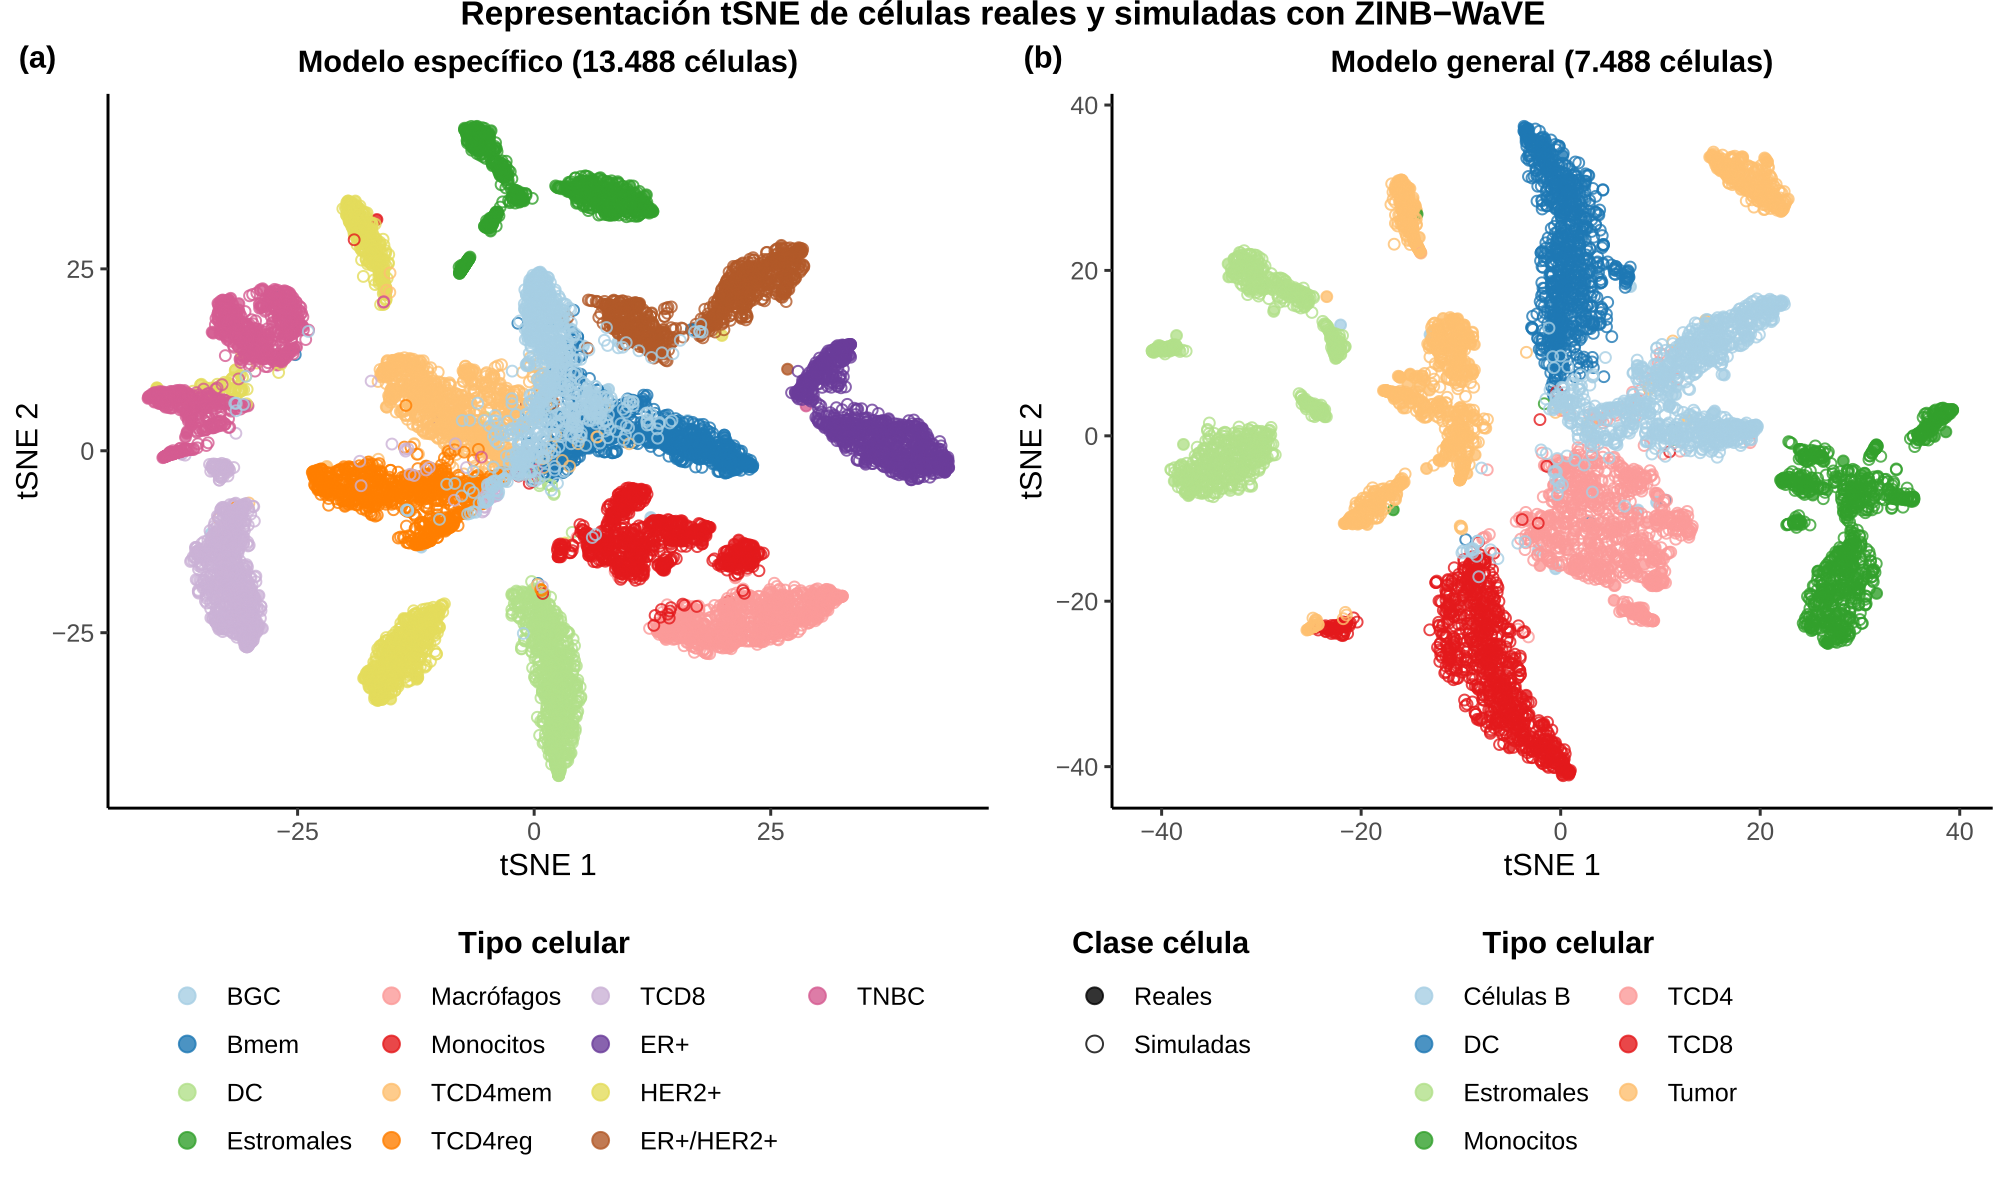
\includegraphics[width = 12cm]{images/simulSingleCell.png}
  \end{figure}
\end{frame}

\begin{frame}{Matrices de composición celular y modelos}
  \begin{columns}
    \begin{column}{0.5\textwidth}
      \vskip-1mm
      \begin{figure}
        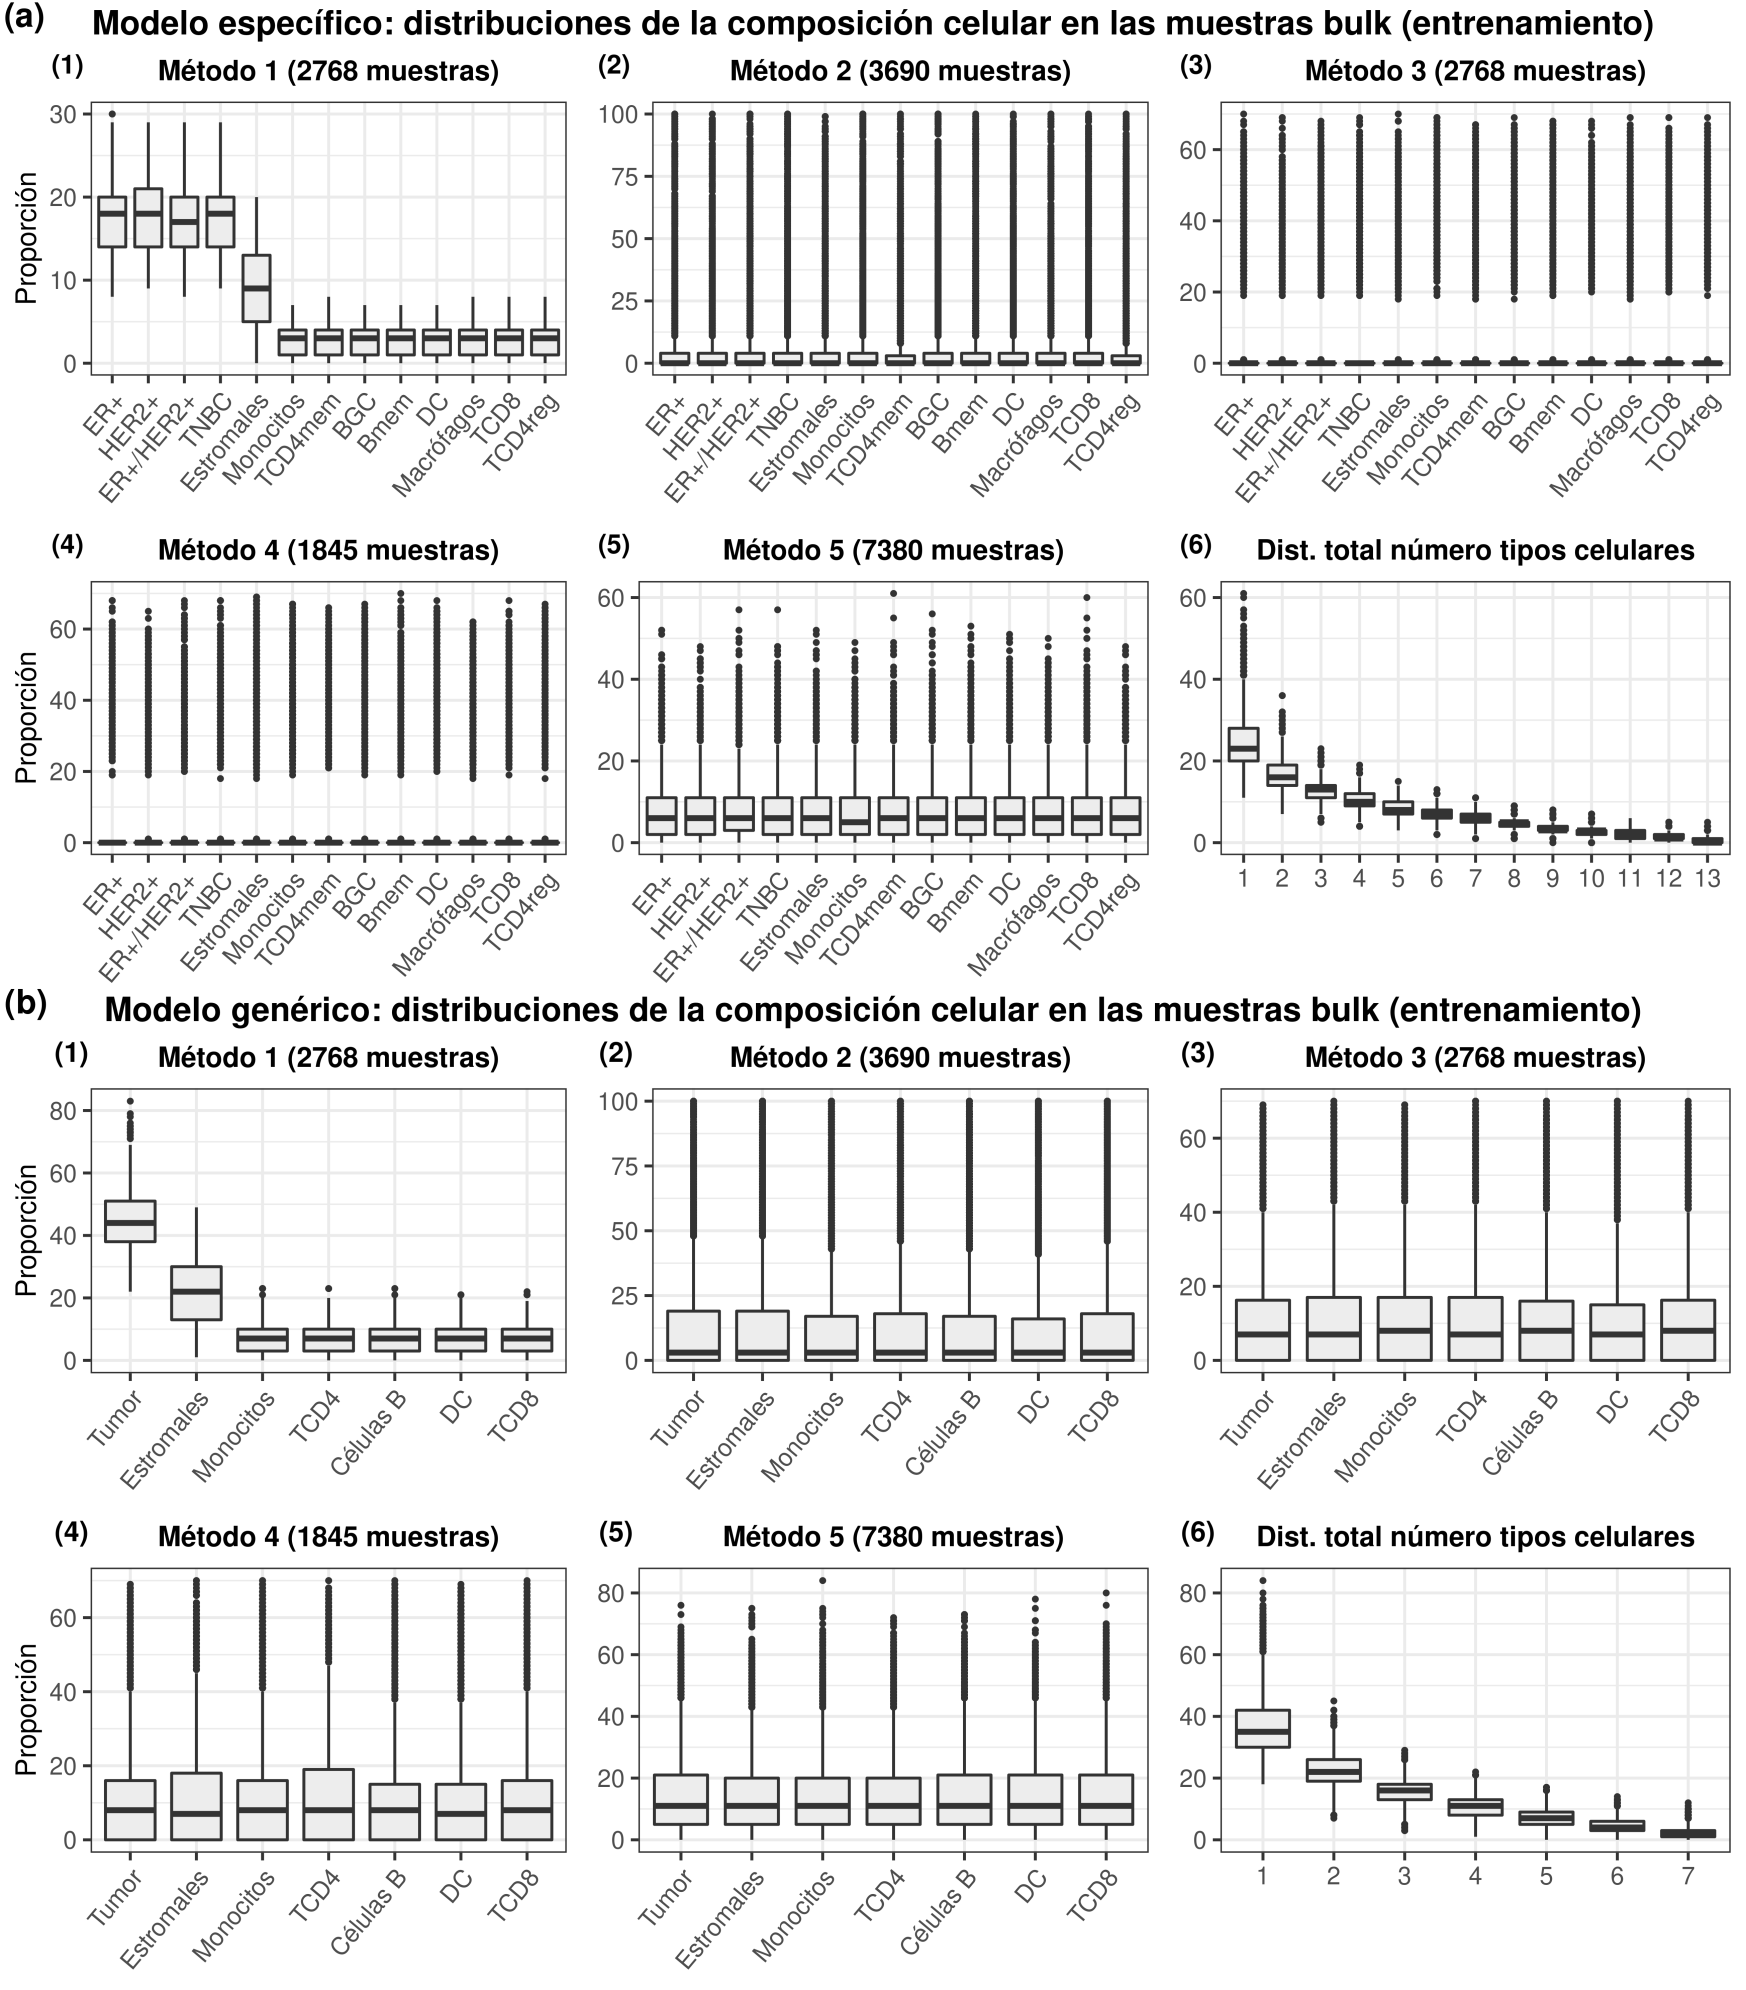
\includegraphics[width=6.7cm]{images/boxplotsFinal.png}
      \end{figure}
    \end{column}
    \begin{column}{0.5\textwidth}
      \begin{alertblock}{Modelos construidos (datos entrenamiento)}
        \begin{enumerate}
          \item Modelo específico 1 $\rightarrow$ solo \textit{bulk}: 18.451 muestras.
          \item Modelo específico 2 $\rightarrow$ solo \textit{single-cell}: 8.992 células.
          \item Modelo específico 3 $\rightarrow$ solo \textit{bulk} + \textit{single-cell}: 18.451 muestras y 8.992 células.
          \item Modelo genérico: solo \textit{bulk} $\rightarrow$ 18.451 muestras.
        \end{enumerate}
      \end{alertblock}
    \end{column}
  \end{columns}
\end{frame}


\begin{frame}[fragile]{Entrenamiento de la Red Neuronal Profunda}

  25 épocas en modelos específicos y 20 épocas en genérico. El resto de parámetros son los establecidos en \texttt{trainDigitalDLSorterModel} por defecto.

  \Fontvi{
    \begin{table}[th]
      \begin{center}
        \begin{tabular}{rcccccc}
          \toprule
          \multirow{2}{*}{}                                                                         &
          \multicolumn{2}{c}{\textbf{KLD}}                                                          &
          \multicolumn{2}{c}{\textbf{Precisión}}                                                    &
          \multicolumn{2}{c}{\textbf{MAE}}                                                                                                                   \\
          Conjunto de datos                                                                         & {Entr.} & {Test} & {Entr.} & {Test} & {Entr.} & {Test} \\
          \midrule
          \rowcolor<3>{OrangeBackground} \textbf{Modelo específico 1 (\textit{bulk})}               & 0,0515  & 0,0751 & 0,7442  & 0,885  & 0,015   & 0,014  \\
          \rowcolor<2>{OrangeBackground} \textbf{Modelo específico 2 (\textit{sc})}                 & 0,0289  & 0,5718 & 1       & 0,6131 & 7,6197  & 0,0465 \\
          \rowcolor<3>{OrangeBackground} \textbf{Modelo específico 3 (\textit{bulk} + \textit{sc})} & 0,0445  & 0,0385 & 0,7953  & 0,8101 & 0,0123  & 0,0112 \\
          \rowcolor<4>{OrangeBackground} \textbf{Modelo genérico (\textit{bulk})}                   & 0,0222  & 0,0154 & 0,9051  & 0,9629 & 0,0186  & 0,0112 \\
          \bottomrule
        \end{tabular}
      \end{center}
    \end{table}
  }
  \begin{itemize}
    \item \alert<2>{Modelo específico 2 con los peores resultados, gran sobreajuste $\rightarrow$ necesidad de incluir muestras \textit{bulk}.}
    \item \alert<3>{Modelo específico 3 superior al Modelo específico 1 $\rightarrow$ necesaria una comparativa más profunda.}
    \item \alert<4>{Modelo genérico con las mejores puntuaciones $\rightarrow$ problema más sencillo.}
  \end{itemize}

\end{frame}


\begin{frame}{Evaluación del desempeño de la deconvolución: modelos específicos}
  \begin{columns}
    \begin{column}{0.5\textwidth}
      \begin{figure}
        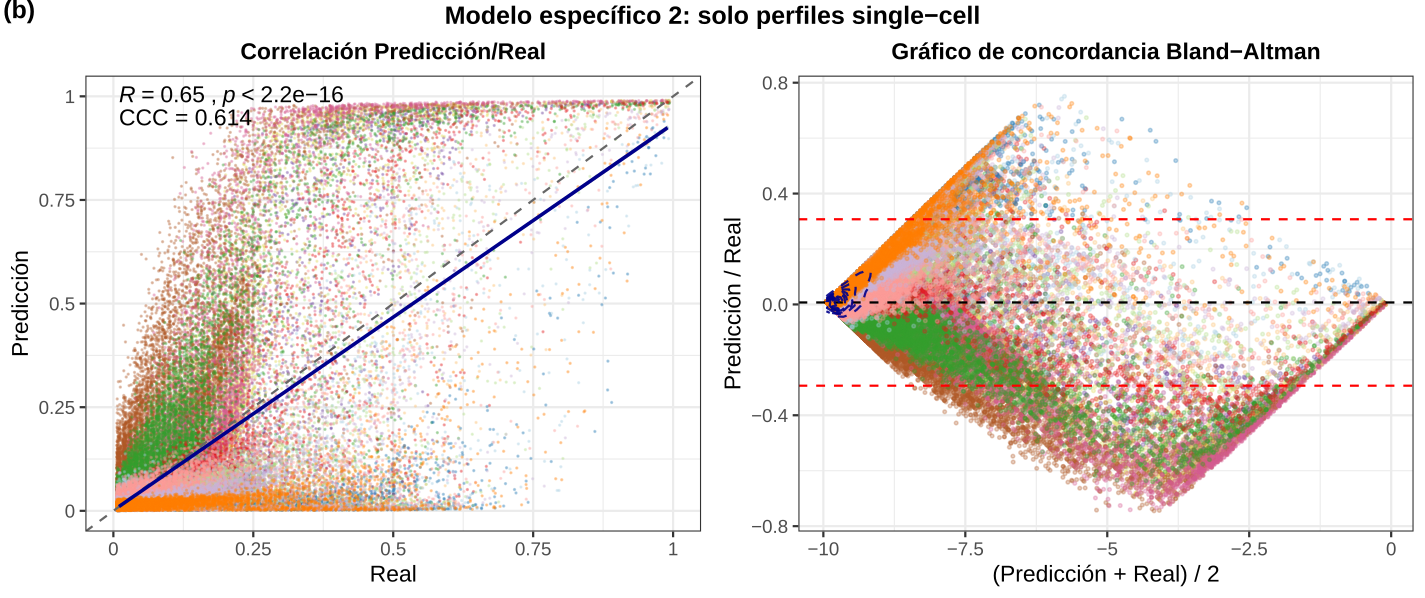
\includegraphics[width=7cm]{images/modelo_especifico_2_2.png}
      \end{figure}
    \end{column}
    \begin{column}{0.5\textwidth}
      % \begin{textblock*}{3cm}(12cm,2cm)
      \Fonteight{
        \begin{alertblock}{Resultados}
          \begin{itemize}
            \item Modelo específico 2: peores resultados $\rightarrow$ $R$ = 0,65 y CCC = 0,614
            \item Modelos específicos 1 y 3: similares, ligeramente superior el 1.
          \end{itemize}
        \end{alertblock}
      }
      % \end{textblock*}
    \end{column}
  \end{columns}

  \begin{columns}
    \begin{column}{0.5\textwidth}
      \begin{figure}
        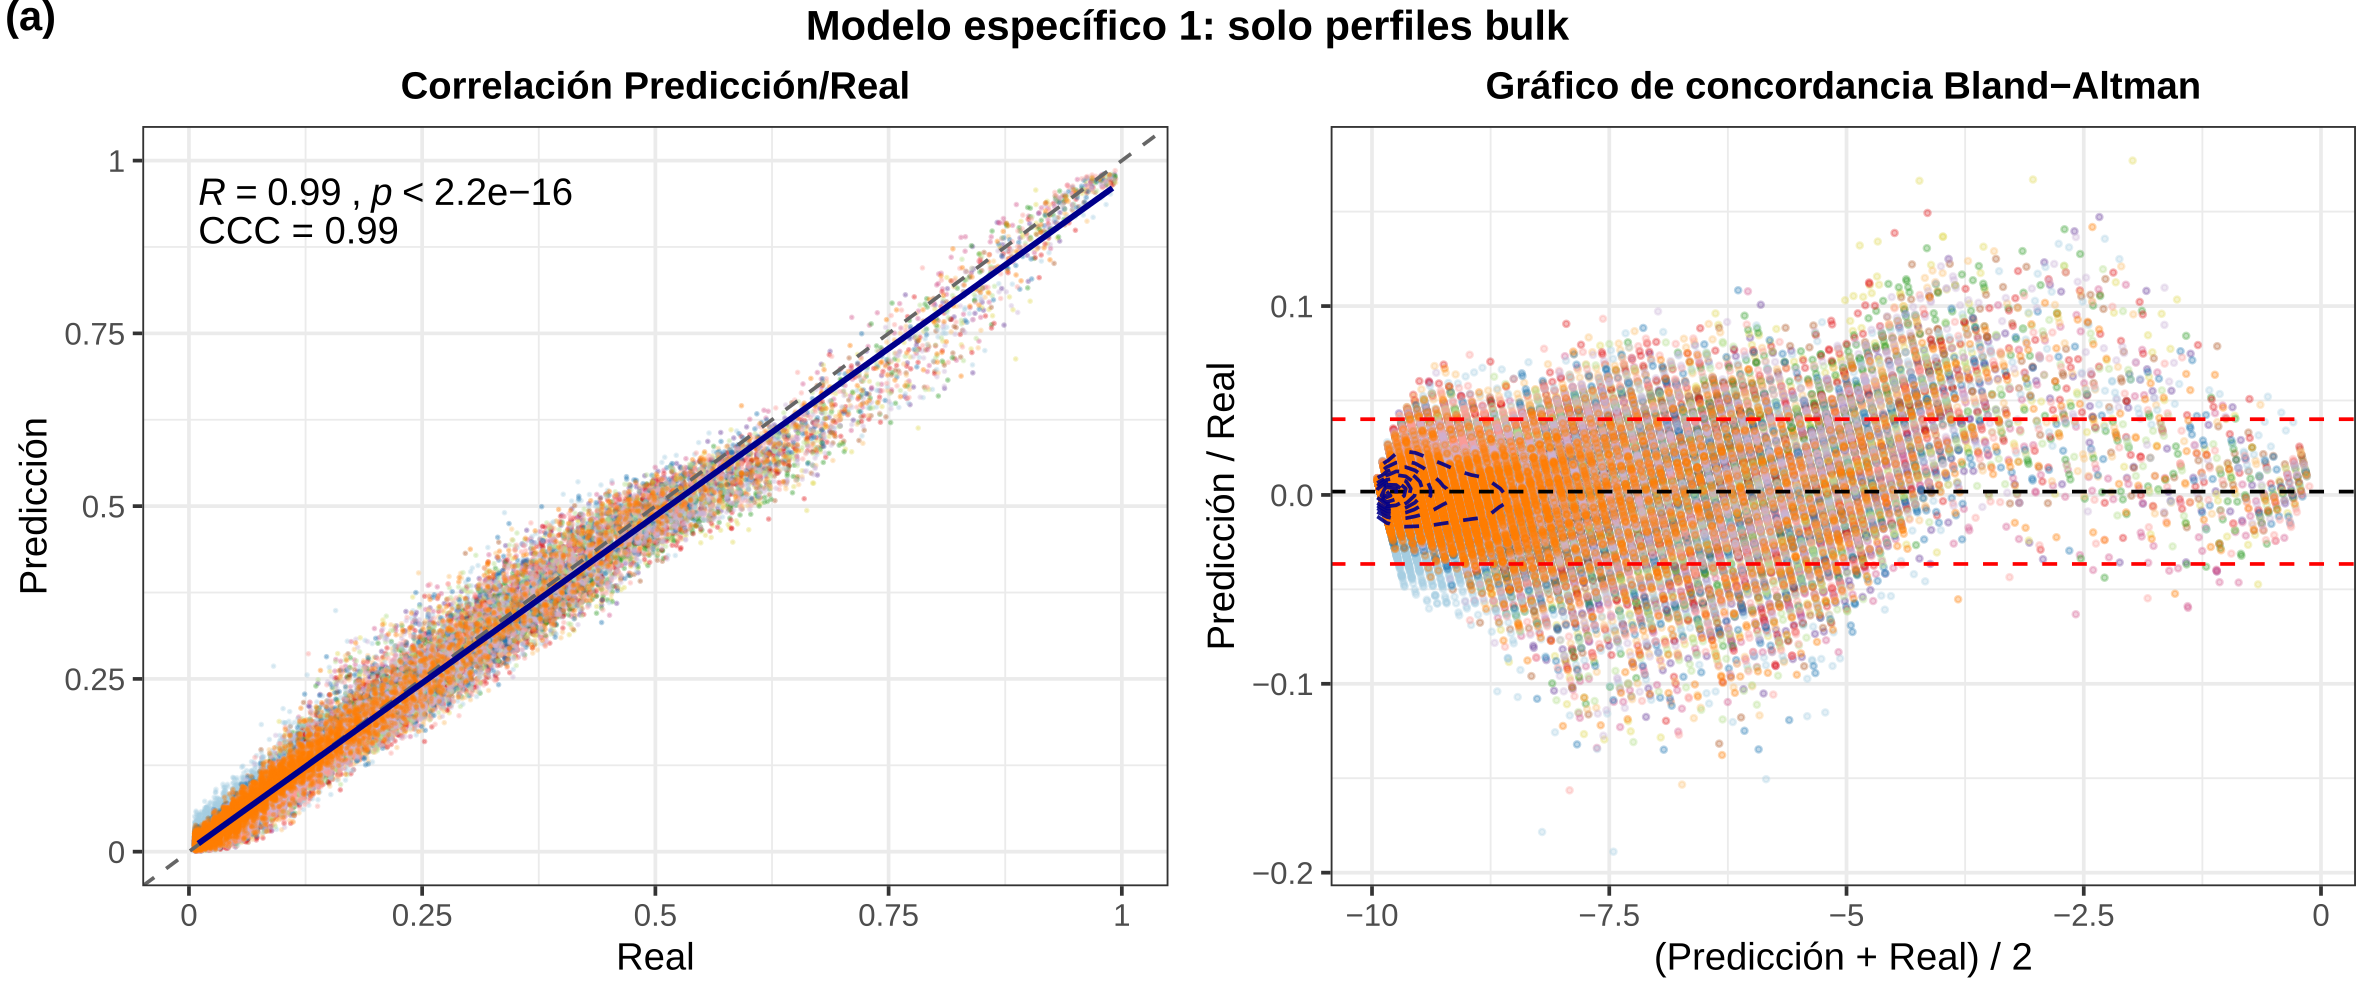
\includegraphics[width=7cm]{images/modelo_especifico_1.png}
      \end{figure}
    \end{column}
    \begin{column}{0.01\textwidth}
      \begin{figure}
        
\includegraphics[width=0.5cm]{images/approx.png}
      \end{figure}
    \end{column}
    \begin{column}{0.5\textwidth}
      \begin{figure}
        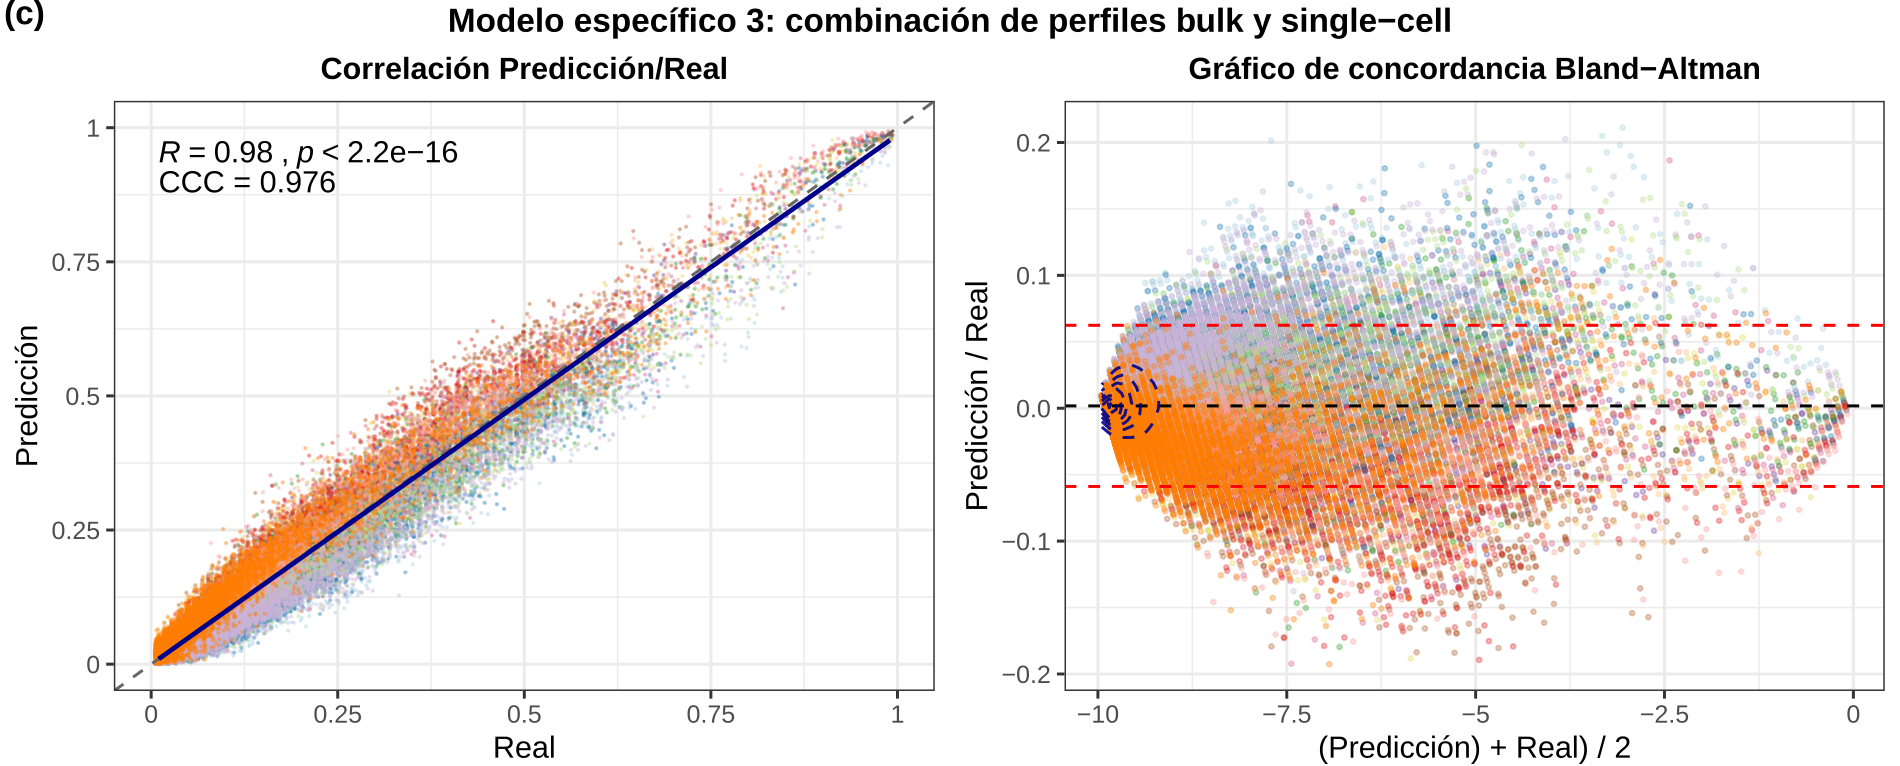
\includegraphics[width=7cm]{images/modelo_especifico_3_1mod.png}
      \end{figure}
    \end{column}
  \end{columns}
\end{frame}


\begin{frame}{Modelo específico 1 vs Modelo específico 3}
  \begin{overlayarea}{\linewidth}{1\textheight}
    \begin{figure}
      \centering
      \only<1>{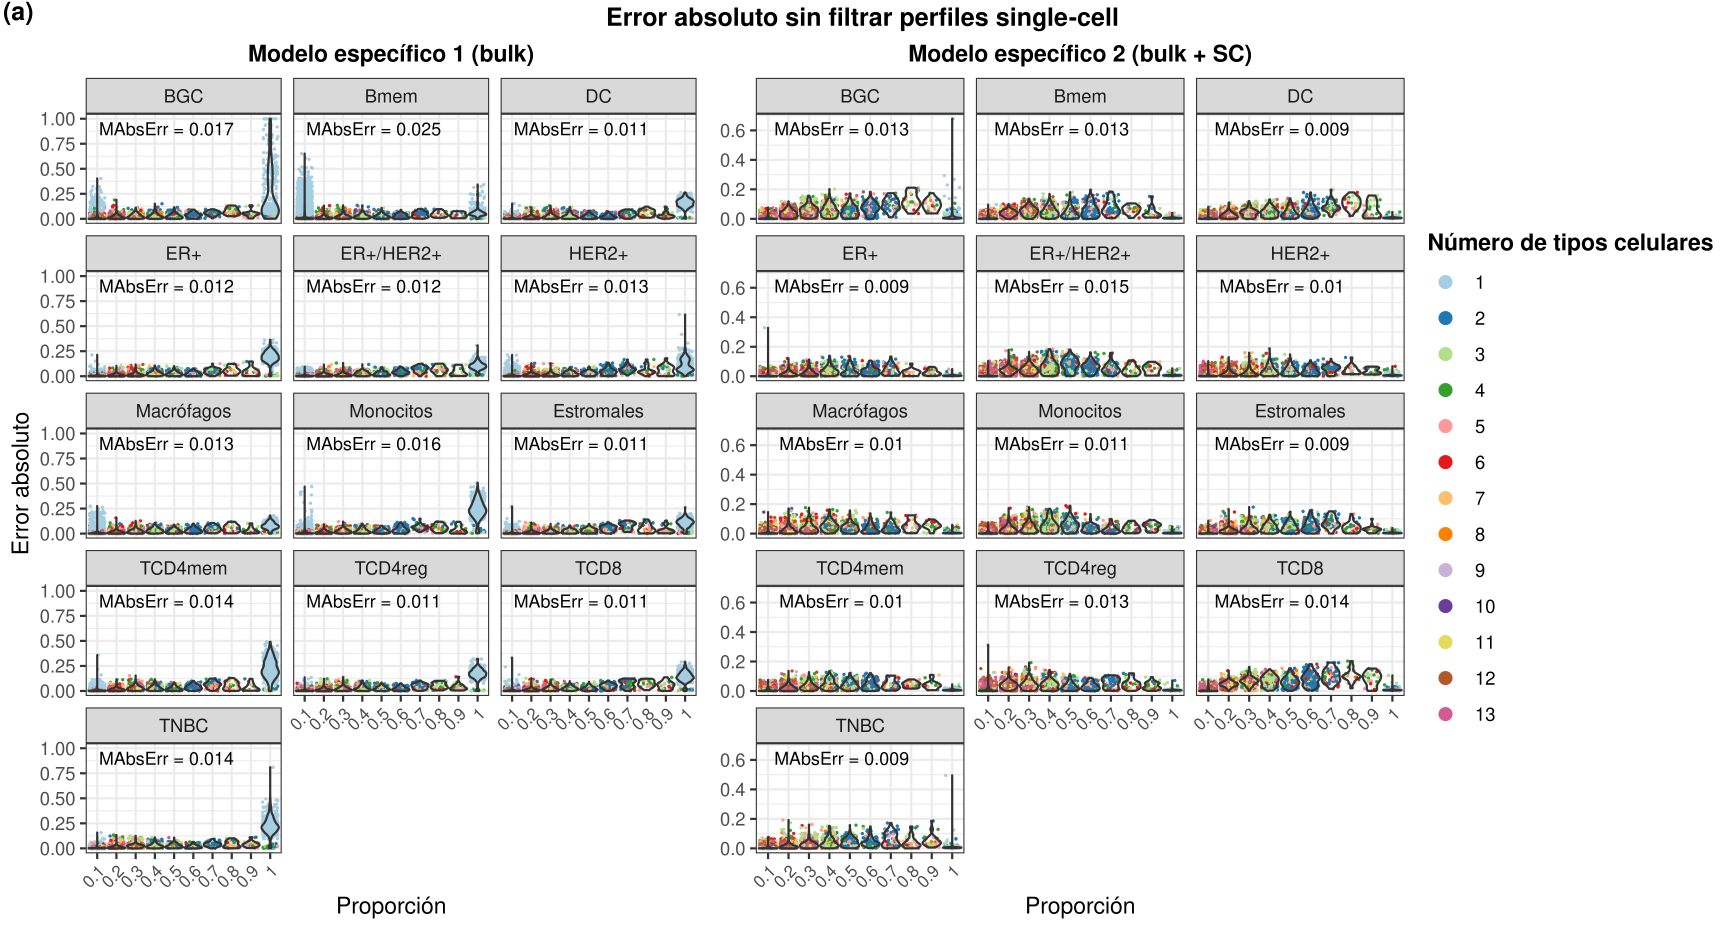
\includegraphics[width=12cm]{images/sinFiltrarSC_2_1.png}}
      \only<2>{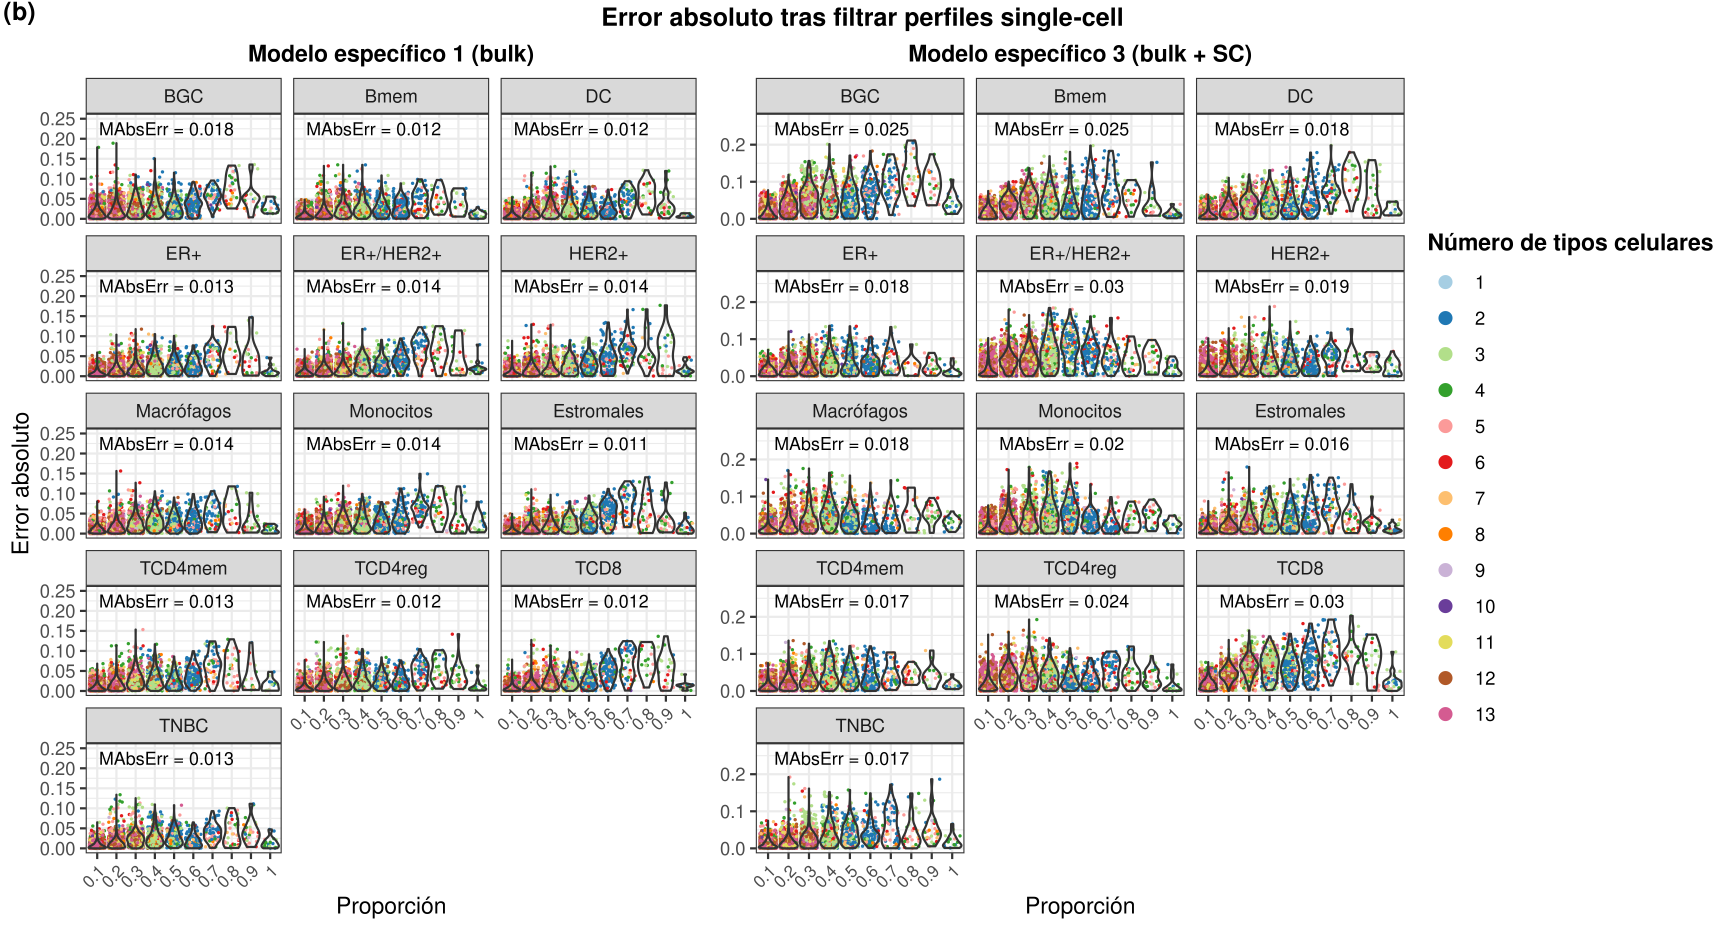
\includegraphics[width=12cm]{images/filtradoSC_2.png}}
    \end{figure}
    \vskip-1.2em
    \begin{itemize}[<alert@+>]
      \item Modelo entrenado con \textit{single-cell} + \textit{bulk} $\rightarrow$ superior sin filtrar perfiles \textit{single-cell}.
      \item Modelo entrenado solo con \textit{bulk} $\rightarrow$ superior retirando los perfiles \textit{single-cell}.
    \end{itemize}
  \end{overlayarea}
\end{frame}

\begin{frame}{Modelo específico 1}
  \begin{columns}
    \begin{column}{0.6\textwidth}
      \begin{figure}
        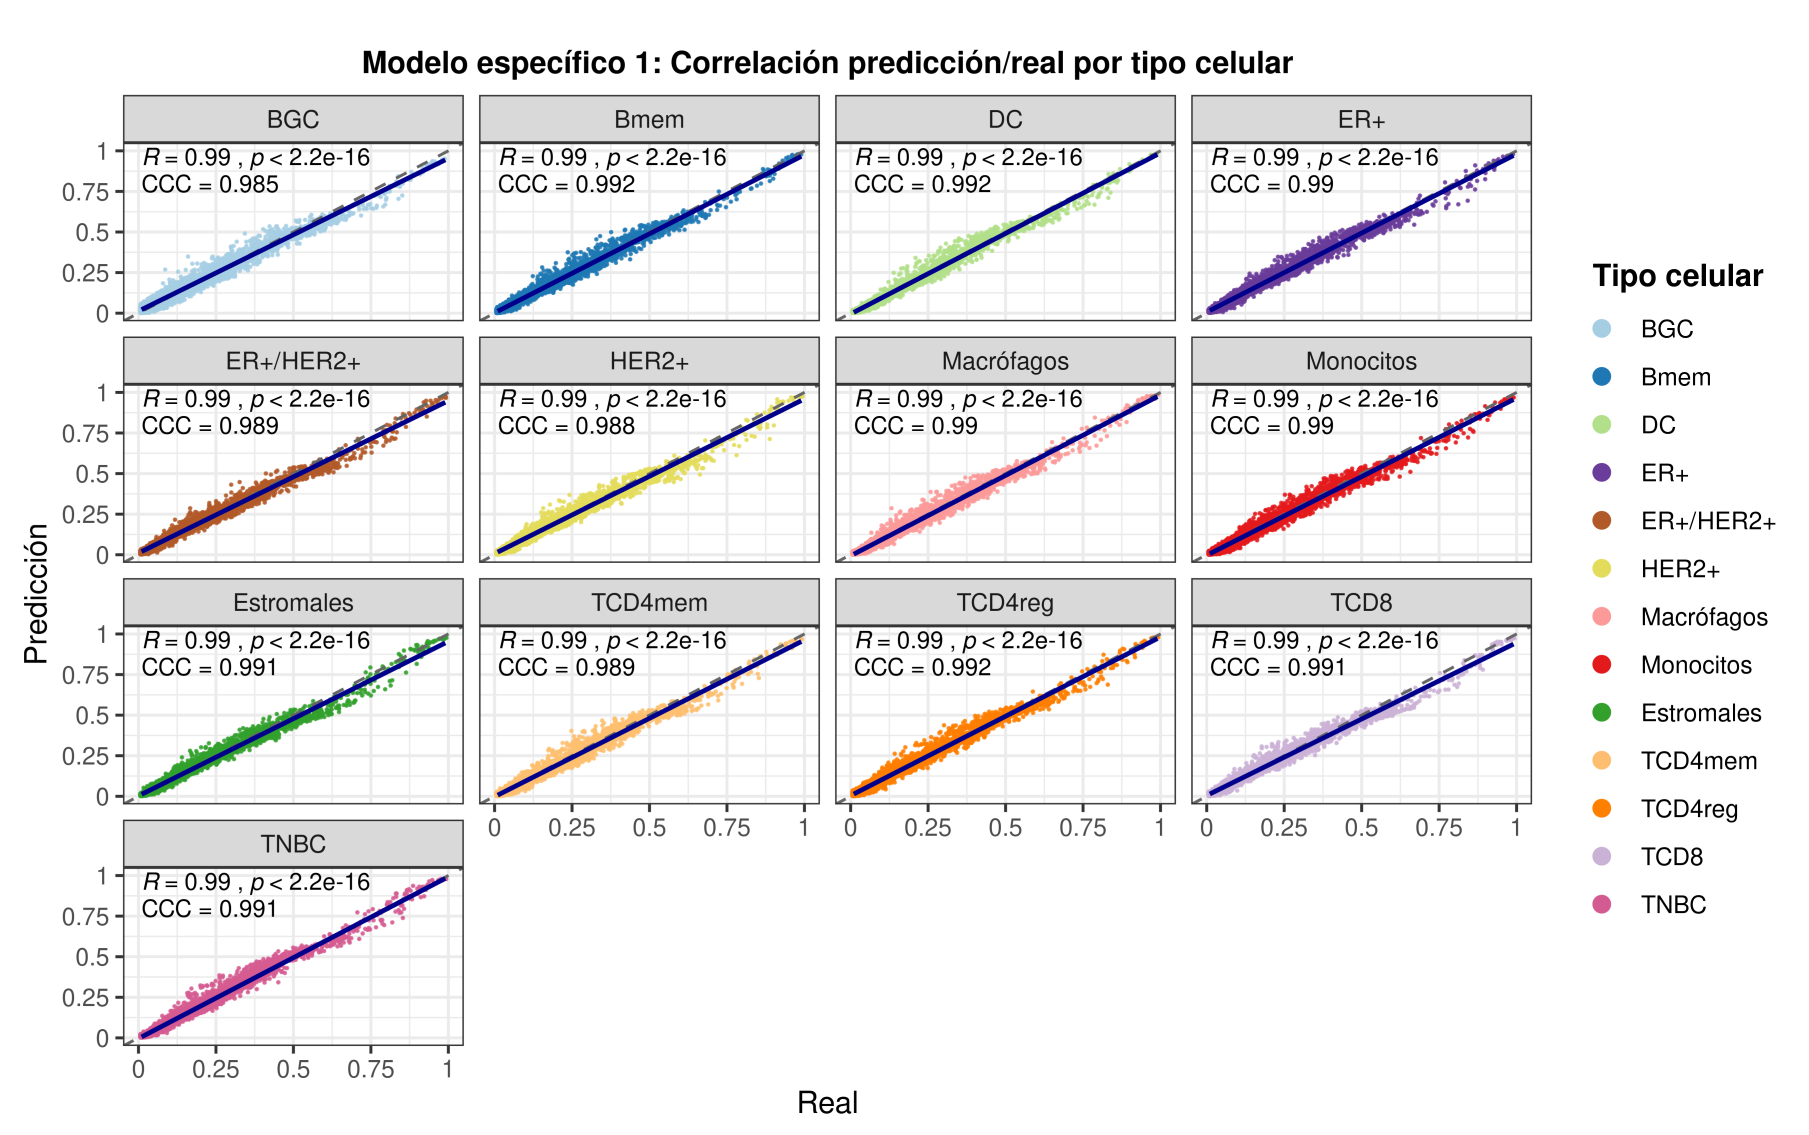
\includegraphics[width=9cm]{images/modelo1Corr.png}
      \end{figure}
    \end{column}
    \begin{column}{0.4\textwidth}
      \begin{itemize}
        \item Niveles de correlación cercanos a 0,99 tanto en $R$ como en CCC.
        \item Errores mayores en tipos celulares tumorales y BGC.
      \end{itemize}
    \end{column}
  \end{columns}

  \begin{beamercolorbox}[sep=0.2cm,center]{coloredboxstuff}
    Buen desempeño general en todos los tipos celulares.
  \end{beamercolorbox}
\end{frame}

\begin{frame}{Modelo genérico}

  \begin{figure}
    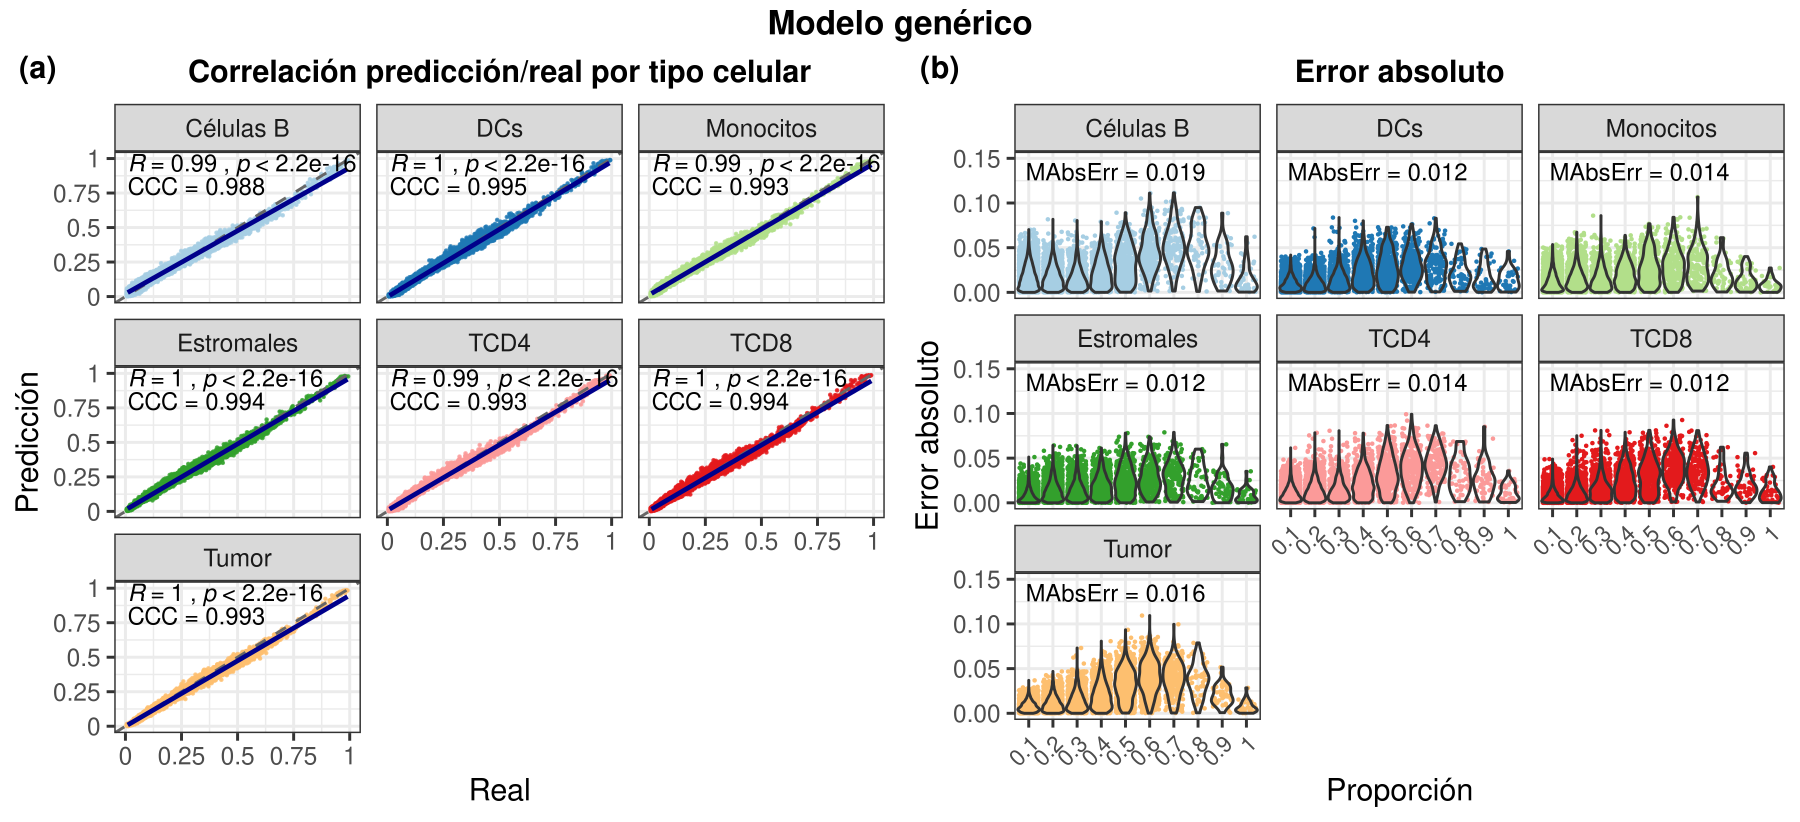
\includegraphics[width=12cm]{images/modeloGenerico_2_cut.png}
  \end{figure}

  \vskip-2mm

  \begin{itemize}
    \item Mismas tendencias que las observadas en el modelo específico.
    \item Errores menores en general.
  \end{itemize}


  \begin{beamercolorbox}[sep=0.2cm,center]{coloredboxstuff}
    Buen desempeño general en todos los tipos celulares.
  \end{beamercolorbox}
\end{frame}

\begin{frame}{Modelos de deconvolución sobre datos \textit{bulk} reales}
  Datos \textit{bulk RNA-seq} de cáncer de mama procedentes del proyecto TCGA (\textit{The Cancer Genome
    Atlas}): 1222 muestras.
  \Fontvi
  \begin{alertblock}{Problema}
    \vskip1mm
    \begin{itemize}
      \item No se tienen las proporciones celulares de las muestras.
      \item \alert<2>{Análisis de correlación entre las proporciones predichas.}
    \end{itemize}
  \end{alertblock}


  \begin{alertblock}{Se espera}
    \vskip1mm
    Tipos pro-tumorales correlacionen positivamente con proporciones tumorales:
    \begin{itemize}
      \item Linfocitos T reguladores
      \item Macrófagos.
    \end{itemize}

    Tipos anti-tumorales correlacionen negativamente con proporciones tumorales:
    \begin{itemize}
      \item Células B de memoria.
      \item Linfocitos T CD8+.
    \end{itemize}
  \end{alertblock}

\end{frame}

\begin{frame}{Modelo específico sobre datos TCGA}
  \begin{columns}
    \begin{column}{0.55\textwidth}
      \begin{overlayarea}{\linewidth}{1\textheight}
        \begin{figure}
          \centering
          \only<1>{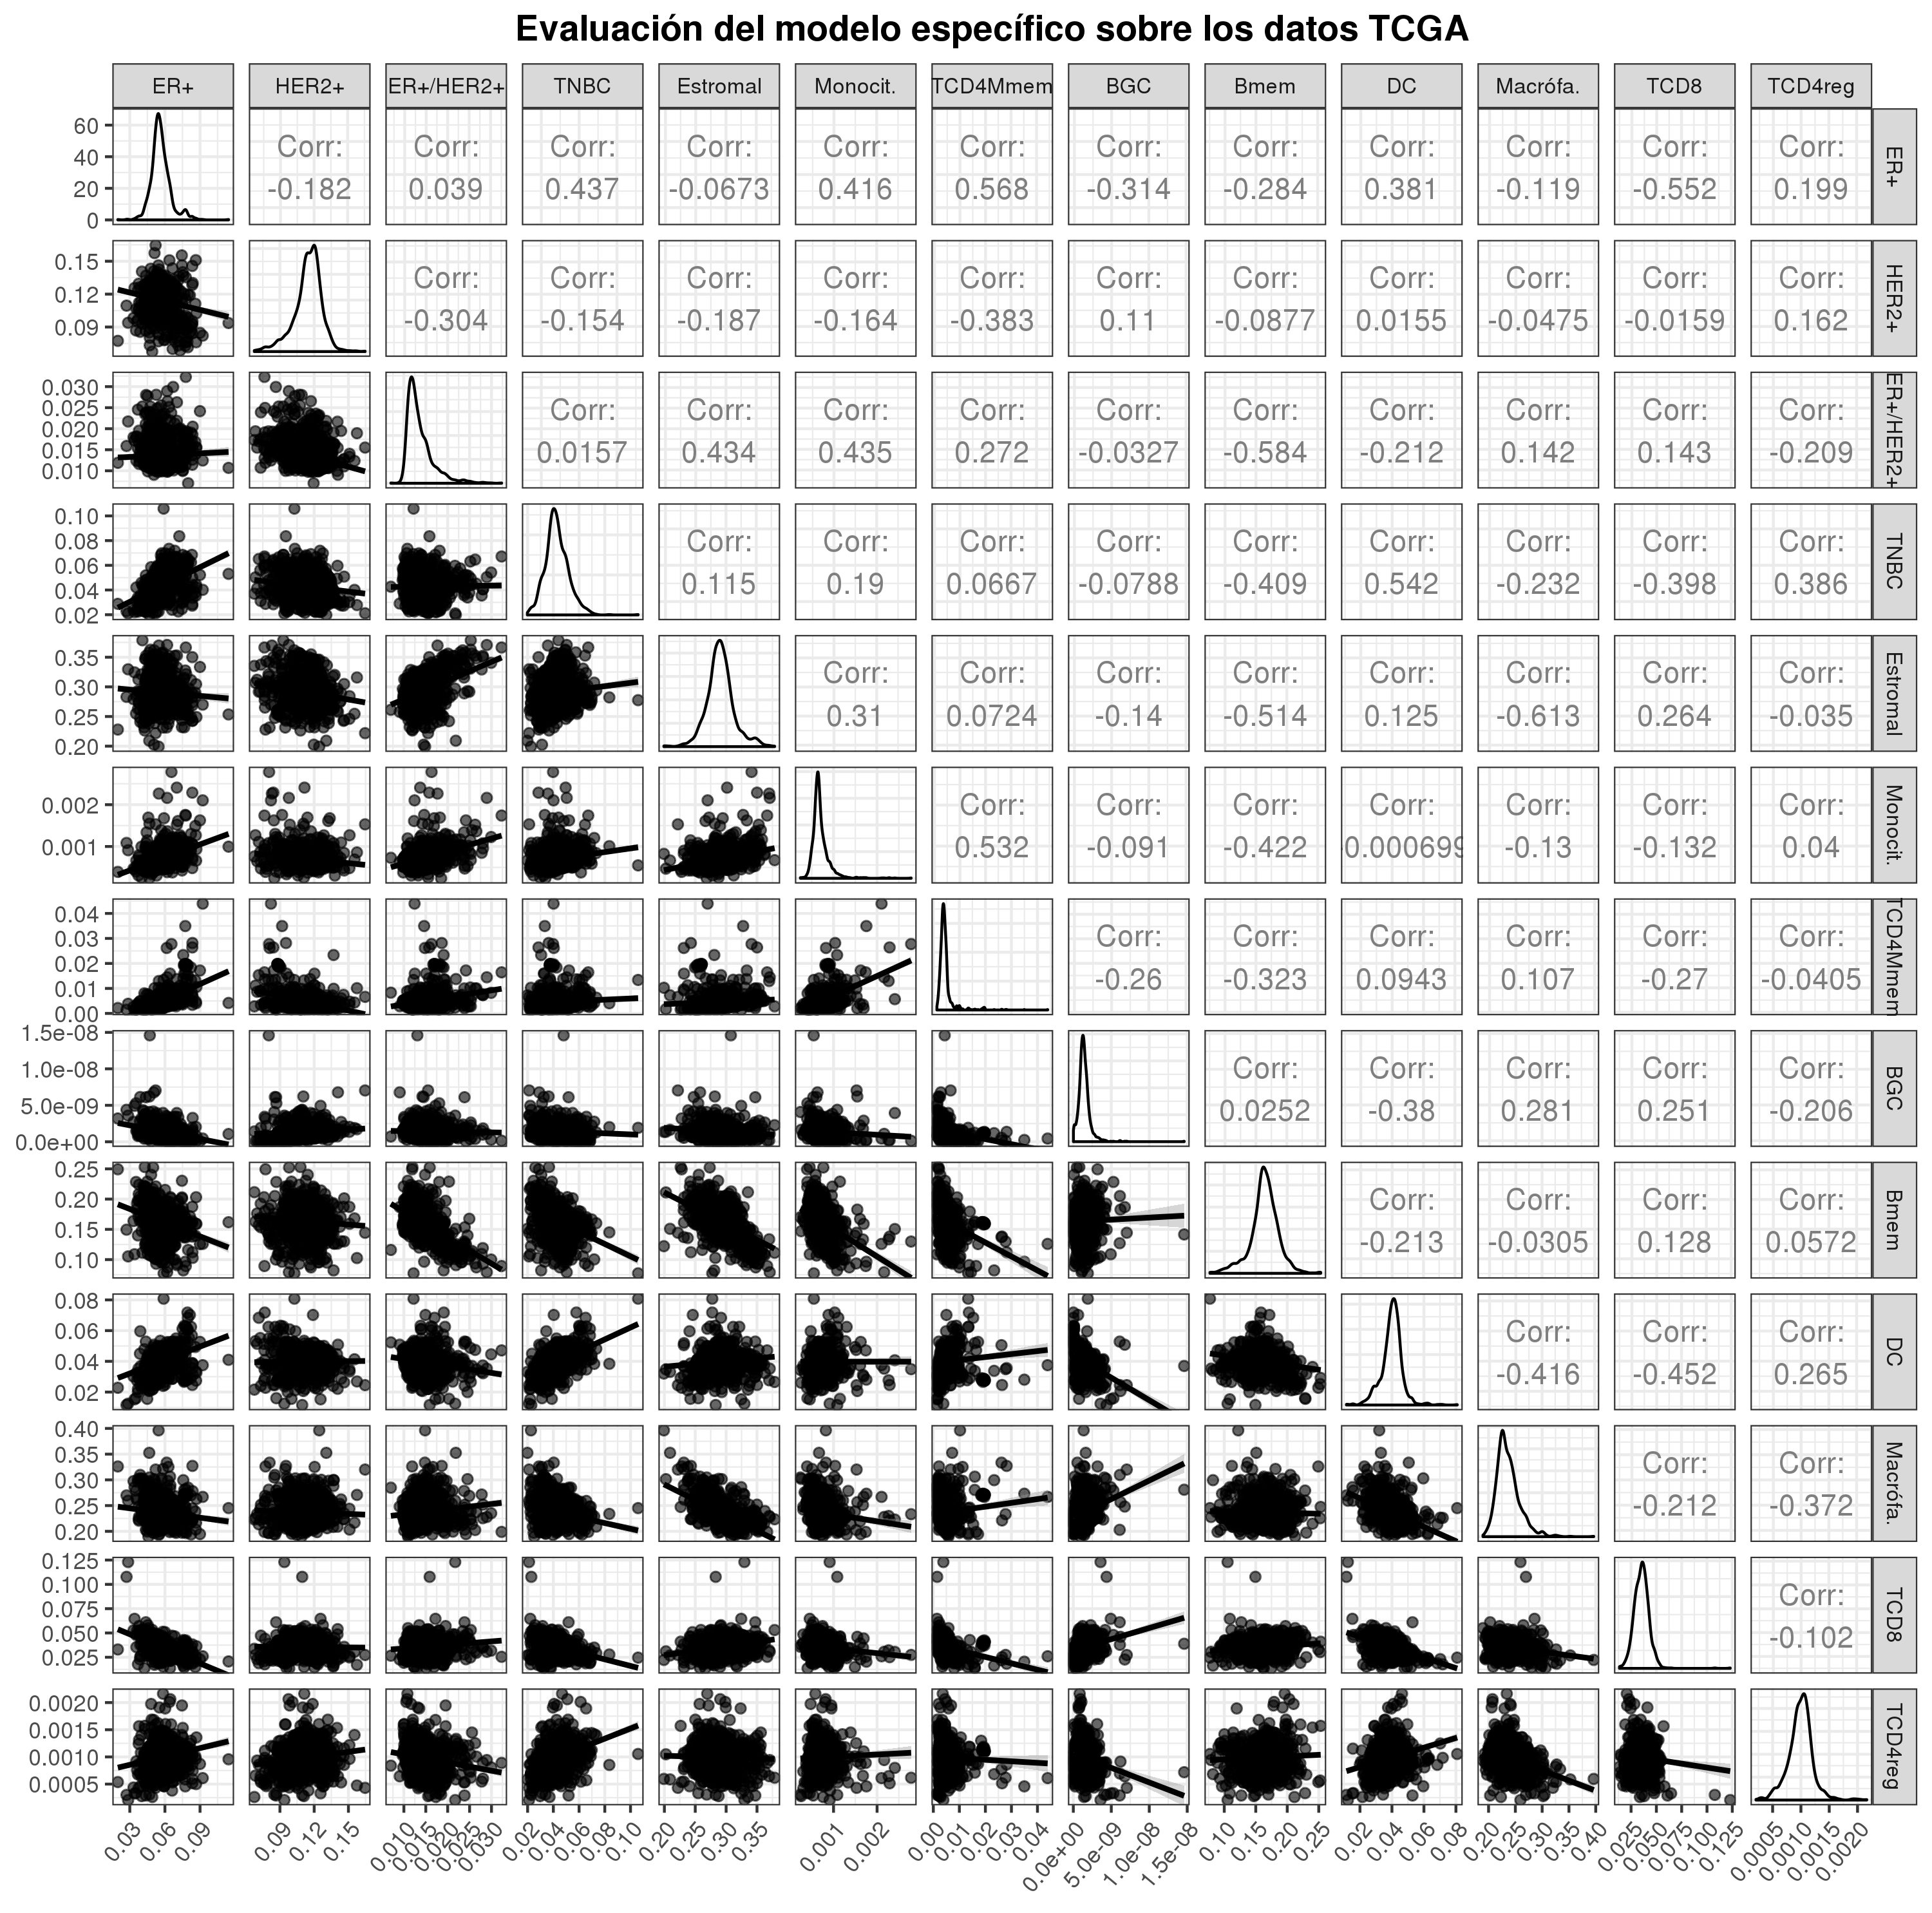
\includegraphics[width=7.5cm]{images/totalEspecifico.png}}
          \only<2>{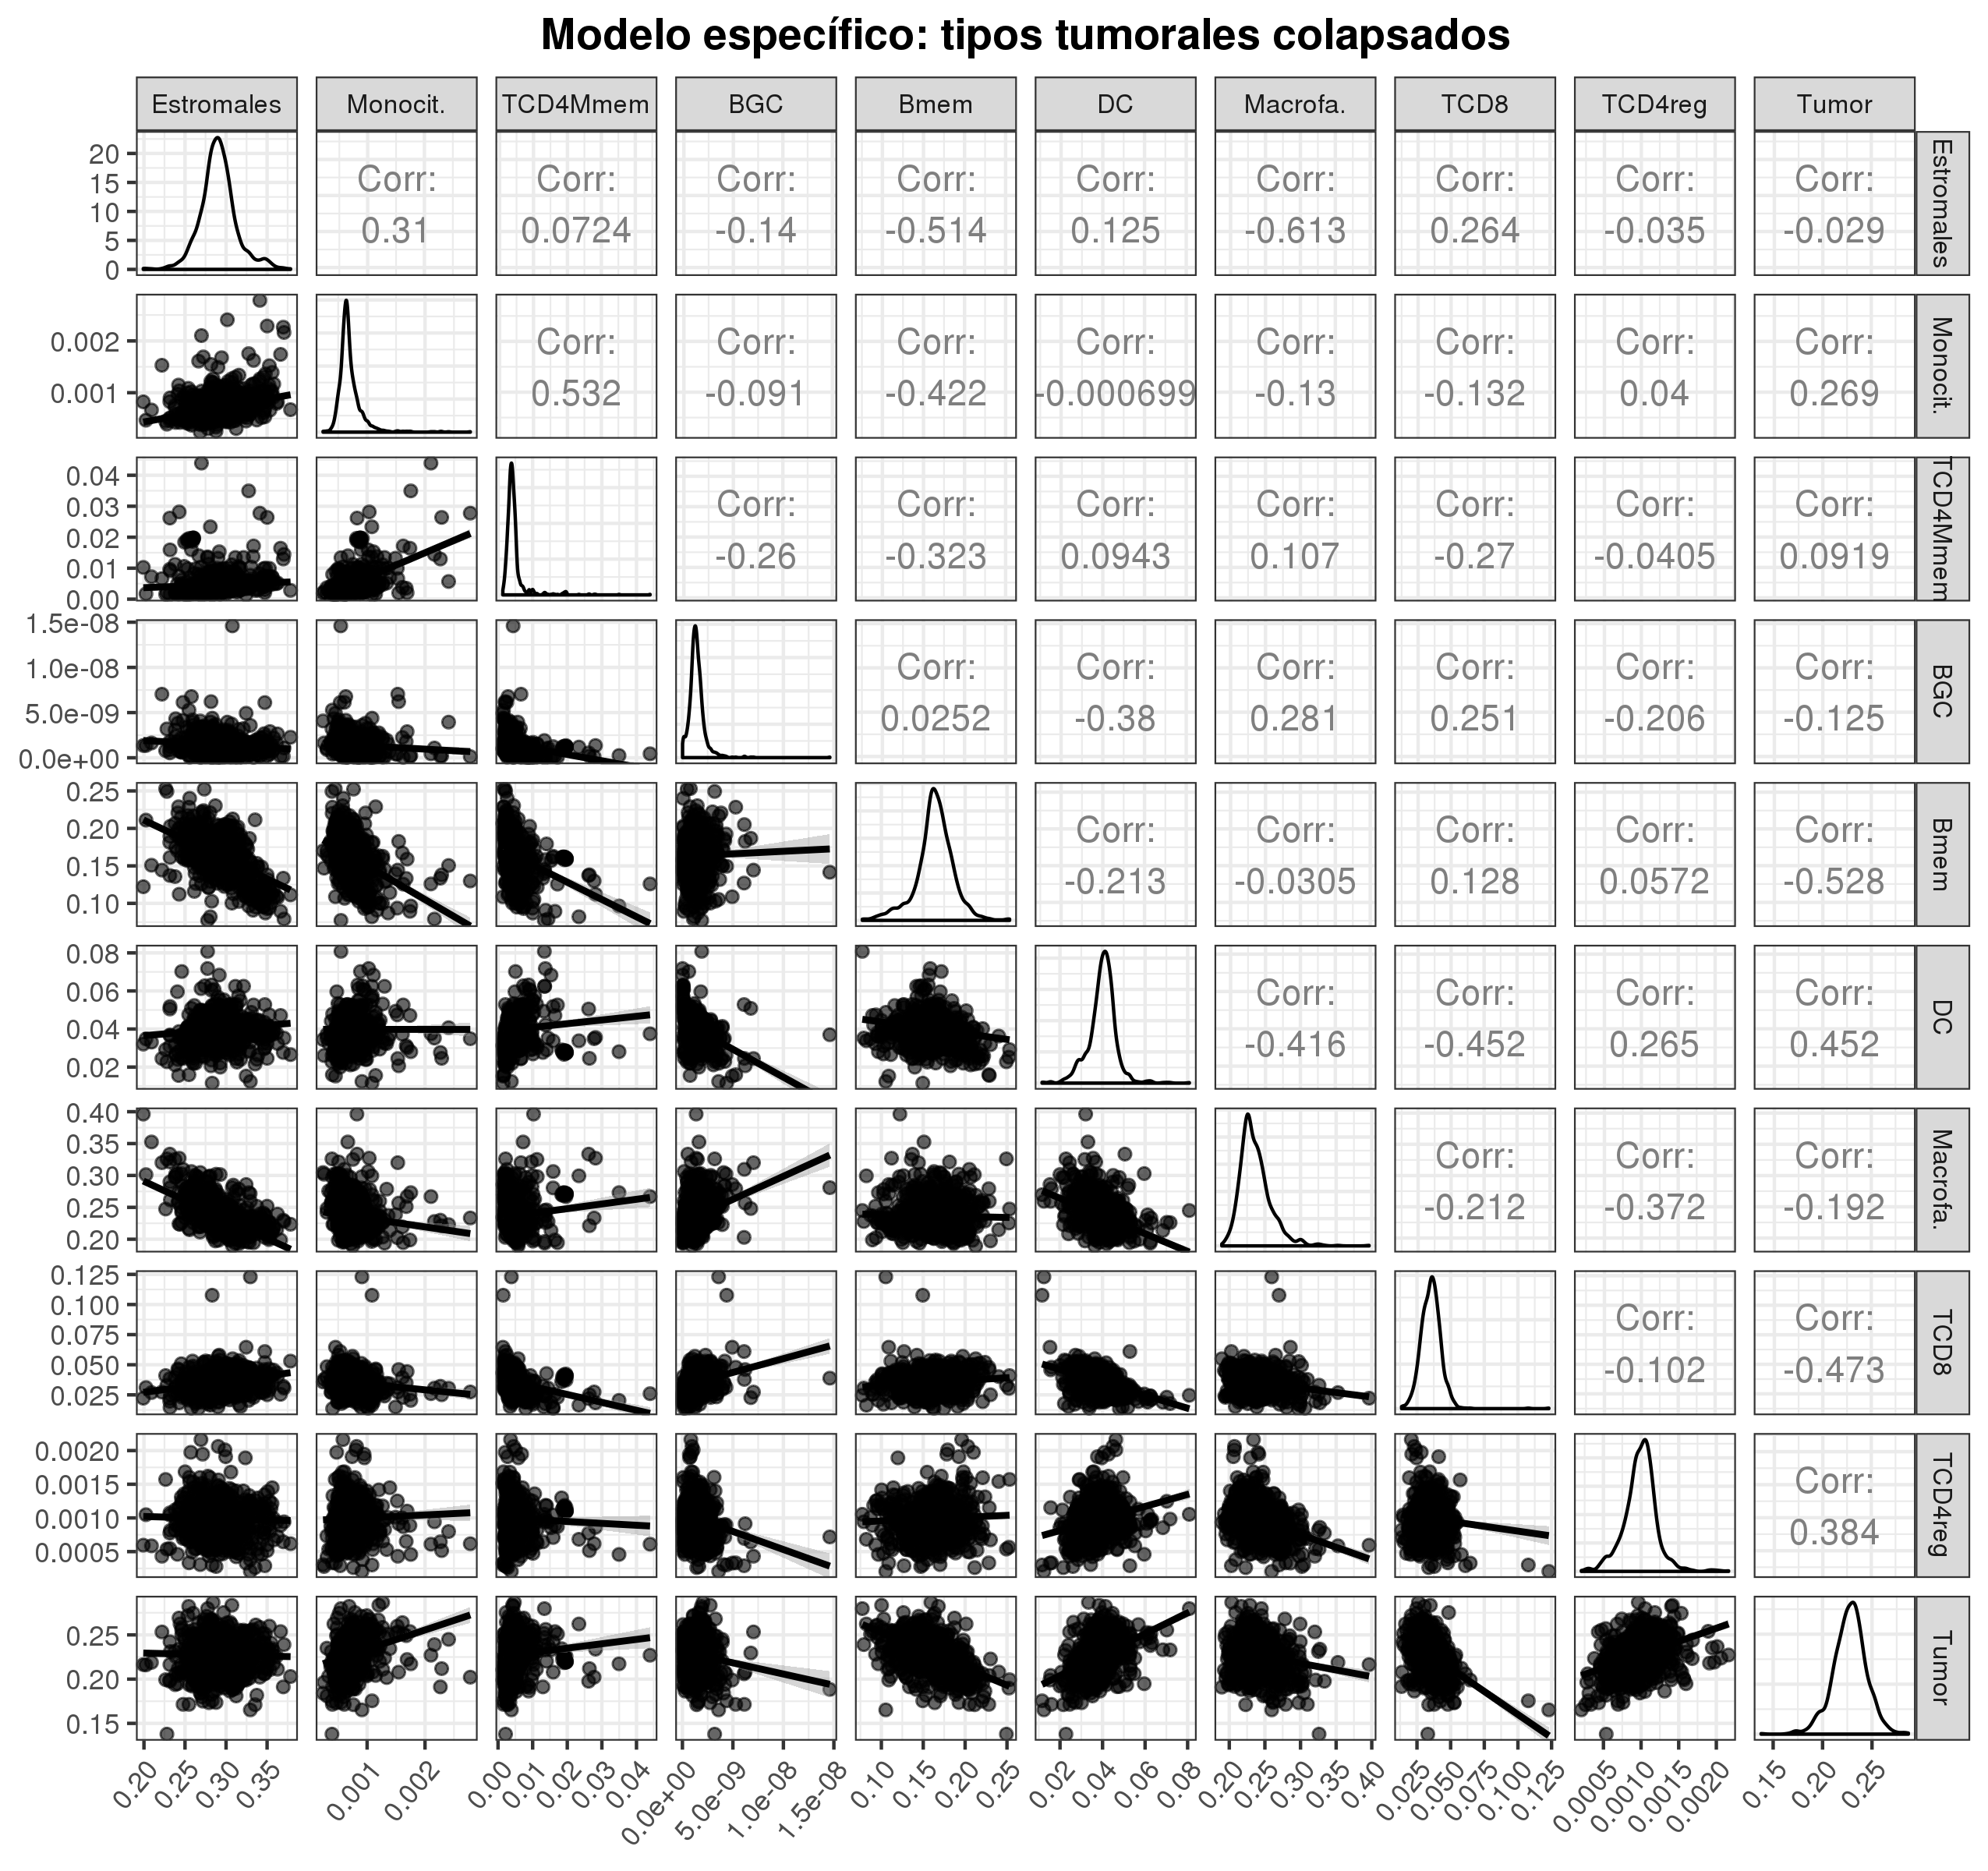
\includegraphics[width=7.5cm]{images/especificoSimplificadoSetTumor.png}}
        \end{figure}
      \end{overlayarea}
    \end{column}

    \begin{column}{0.5\textwidth}
      \begin{itemize}
        \item Lincofitos T CD8+ y linfocitos B de memoria $\rightarrow$ anticorrelacionan con 3 de los 4 subtipos de cáncer.
        \item Linfocitos T CD4+ reguladores: correlacionan positivamente con 3 de los 4 subtipos de cáncer.
      \end{itemize}
      \begin{alertblock}{Problema}
        \vskip0.1mm
        ER+/HER2+ no es predicho según lo esperado. $\rightarrow$ proporciones medias de 1,14\%.
      \end{alertblock}
      \begin{alertblock}{Solución}
        \vskip0.1mm
        Uso del argumento \texttt{simplify.set} agrupando los 4 subtipos intrínsecos de cáncer bajo la etiqueta 'Tumor'.
      \end{alertblock}
    \end{column}
  \end{columns}


\end{frame}


\begin{frame}{Modelo genérico sobre datos TCGA}
  \begin{columns}
    \begin{column}{0.6\textwidth}
      \begin{figure}
        \centering
        \vskip-0.5em
        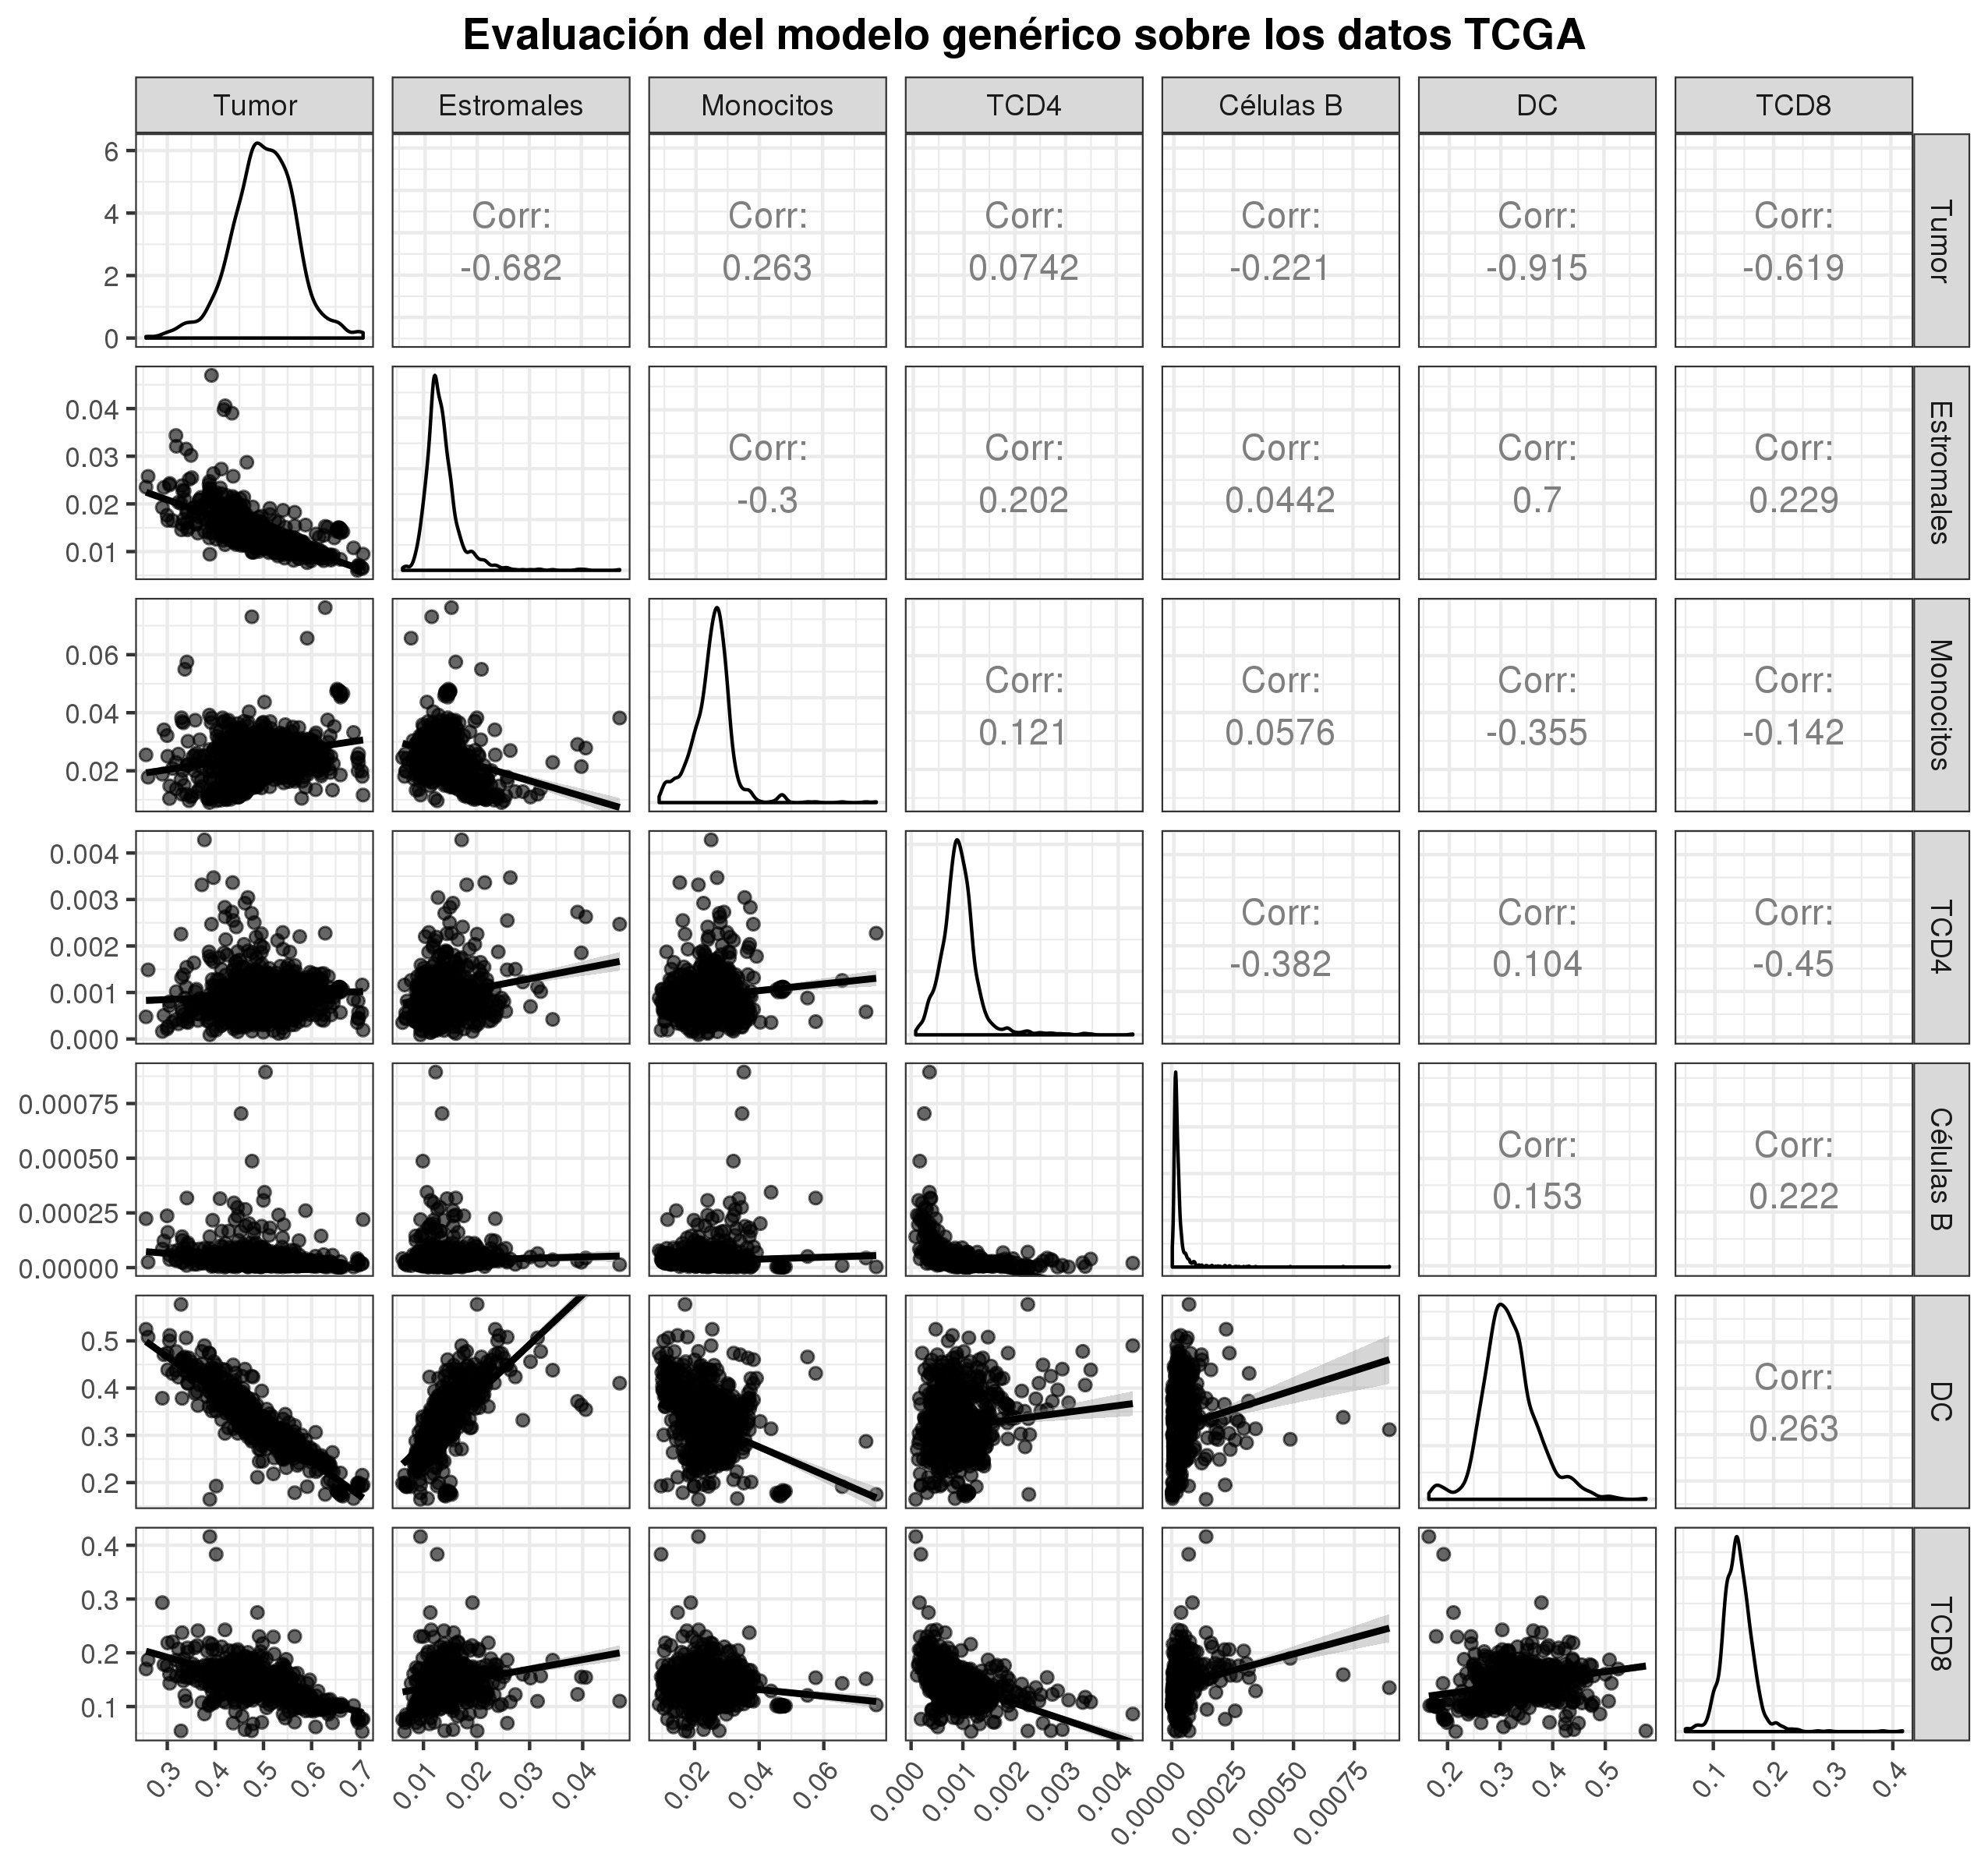
\includegraphics[width=8cm]{images/genericoTotal.png}
      \end{figure}    
    \end{column}
    \begin{column}{0.5\textwidth}
      \begin{itemize}
        \item Mismas tendencias
        \begin{itemize}
          \item Lincofitos T CD8+ y linfocitos B de memoria $\rightarrow$ anticorrelacionan con la proporción tumoral.
          \item Linfocitos T CD4+ reguladores: correlacionan positivamente con la proporción tumoral.
        \end{itemize}
        \item Consenso entre ambos modelos excepto en las células dendríticas: posible problema en los datos de entrenamiento.
      \end{itemize}
    \end{column}
  \end{columns}
\end{frame}


%%%%%%%%%%%%%%%%%%%%%%%%%%%%%%%%%%%%%%%%%%%%%%%%%%%%%%%%%%%%%%%%%%%%%%%%%%%%%%%%%%%%
%%%%%%%%%%%%%%%%%%%%%%%%%%%%%%%%%%%% CONCLUSIONES %%%%%%%%%%%%%%%%%%%%%%%%%%%%%%%%%%
%%%%%%%%%%%%%%%%%%%%%%%%%%%%%%%%%%%%%%%%%%%%%%%%%%%%%%%%%%%%%%%%%%%%%%%%%%%%%%%%%%%%

\section[Conclusiones y trabajo futuro]{Conclusiones y trabajo futuro}

\begin{frame}{digitalDLSorter como método de deconvolución}
  \begin{alertblock}{Resultados obtenidos}
    
  \end{alertblock}

  \begin{alertblock}{Limitaciones y trabajo futuro}
    
  \end{alertblock}
  
\end{frame}


\begin{frame}{digitalDLSorteR como paquete de R}
  \begin{alertblock}{Aportaciones}
    
  \end{alertblock}

  \begin{alertblock}{Limitaciones y trabajo futuro}
    
  \end{alertblock}
  
\end{frame}




%--------------------------------------------------------------------------%


\begin{frame}{Referencias}
  \Fonteight
  \hskip-1em
  \begin{itemize}
    \item Blondel VD, Guillaume JL, Lambiotte R and Lefebvre E. (2008). Fast unfolding of
          communities in large networks. \textit{Journal of Statistical Mechanics: Theory and Experiment}.
    \item Girvan M, Newman, MEJ. (2002). Community structure in social and biological networks.
          \textit{Proceedings of the National Academy of Sciences}. 99 (12):7821–7826.
    \item Levine JH, Simonds EF, Bendall SC, Davis KL, Amir ED, Tadmor MD, et al. (2015). Data-driven
          phenotypic dissection of AML reveals progenitor-like cells that correlate with prognosis.
          \textit{Cell}. 162:184–97.
    \item Liu X, Song W, Wong BY, et al. (2019). A comparison framework and guideline of clustering
          methods for mass cytometry data. \textit{Genome Biol}. 20:297–301.
    \item Newman, MEJ. (2006). Modularity and community structure in networks.
          \textit{Proceedings of the National Academy of Sciences}. 103 (23):8577–8582
    \item Weber LM and Robinson MD. (2016). Comparison of clustering methods for high‐dimensional
          single‐cell flow and mass cytometry data. \textit{Cytometry}. 89:1084–1096.
  \end{itemize}
\end{frame}

{\setbeamercolor{palette primary}{fg=white, bg=Blue}
\begin{frame}[standout]
  Gracias por vuestra atención.
\end{frame}
}


\appendix

\begin{frame}[fragile]{Extra}
  \begin{alertblock}{F-measure}
    \begin{align*}
      F(c_i, k_j)    & = \frac{2 \times Pr_{ij} \times Re_{ij}}{Pr_{ij} + Re_{ij}} \\
      F_{mean}(C, K) & = \sum_{ci} \frac{|c_i|}{N} max_{k_j}F(c_i, k_j)
    \end{align*}
  \end{alertblock}

  \vskip-1.5em

  \begin{alertblock}{Normalized Mutual Information}
    \begin{equation*}
      NMI = \frac{I(X;Y)}{\sqrt{H(X)H(Y)}}
    \end{equation*}
  \end{alertblock}

  \vskip-1em

  \begin{alertblock}{Non-redundancy score (NRS)}
    \begin{equation*}
      NRS(A_p) = \sum_{k = 1:c} |coeff(k)| \times eigenvalue(k)
    \end{equation*}


  \end{alertblock}
\end{frame}



\end{document}
